\documentclass[10pt,a4paper,twocolumn,twoside]{article}

% --- Core Packages ---
\usepackage[utf8]{inputenc}
\usepackage[margin=18mm,top=22mm,bottom=22mm]{geometry}
\usepackage{amsmath,amssymb,amsfonts}
\usepackage{algorithmic}
\usepackage{algorithm}
\usepackage{graphicx}
\usepackage{textcomp}
\usepackage{xcolor}
\usepackage{booktabs}
\usepackage{multirow}
\usepackage{tabularx}
\usepackage{url}
\usepackage{fancyhdr}
\usepackage{microtype}
\usepackage[caption=false,font=footnotesize]{subfig}
\usepackage[colorlinks=true,linkcolor=amritaMaroon,citecolor=deepTeal,urlcolor=amritaMaroon]{hyperref}

% Define Custom Palette
\definecolor{amritaMaroon}{HTML}{A4123F}
\definecolor{darkNavy}{HTML}{0F172A}
\definecolor{deepTeal}{HTML}{0F766E}

% Float parameters for clean layout
\renewcommand{\topfraction}{0.95}
\renewcommand{\bottomfraction}{0.95}
\renewcommand{\textfraction}{0.05}
\renewcommand{\floatpagefraction}{0.80}
\renewcommand{\dbltopfraction}{0.95}
\renewcommand{\dblfloatpagefraction}{0.80}

% Header and Footer Styling for Springer Nature Manuscript
\pagestyle{fancy}
\fancyhf{}
\fancyhead[LE,RO]{\textsf{\footnotesize Springer Nature Manuscript --- Under Review (Target: \textit{Journal of Medical Systems} / \textit{Scientific Reports})}}
\fancyhead[RE,LO]{\textsf{\footnotesize S. A. Sakhi et al.: FPDAF for ICU Sepsis Forecasting}}
\fancyfoot[C]{\textsf{\footnotesize\thepage}}
\renewcommand{\headrulewidth}{0.4pt}
\renewcommand{\footrulewidth}{0.4pt}

\begin{document}

\title{\LARGE\textbf{FPDAF: A Federated Personalized Drift-Aware Attention Framework for Privacy-Preserving Early Sepsis Forecasting in Multi-Center Critical Care}\\[0.2cm]
\large\textit{A Resilient, Drift-Adaptive, and Explainable Clinical Decision Support Architecture for Intensive Care Telemetry}}

\author{
\textbf{Sheela Akshar Sakhi}\textsuperscript{1,*}, 
\textbf{Hasini Reddy M}\textsuperscript{1}, 
\textbf{Kousik Sarma Lakkaraju}\textsuperscript{1},\\
\textbf{Haswitha K}\textsuperscript{1}, 
\textbf{V. Chakravarthy}\textsuperscript{1}, 
\textbf{G. R. Ramya}\textsuperscript{1}, 
\textbf{Vandhana S}\textsuperscript{1}\\[0.25cm]
\textsuperscript{1}Department of Computer Science and Engineering, Amrita School of Computing,\\
Amrita Vishwa Vidyapeetham, Coimbatore 641112, Tamil Nadu, India\\[0.15cm]
\small\texttt{\{cb.sc.u4cse23547, cb.sc.u4cse23529, cb.sc.u4cse23761,\}}\\[-0.05cm]
\small\texttt{\{cb.sc.u4cse23363, cb.sc.u4cse23753\}@cb.amrita.edu}\\[0.1cm]
\small\texttt{\{gr\_ramya, s\_vandhana\}@cb.amrita.edu}\\[0.15cm]
\small\textsuperscript{*}Corresponding author: Sheela Akshar Sakhi (\texttt{cb.sc.u4cse23547@cb.amrita.edu})
}

\date{\today}

\maketitle
\thispagestyle{fancy}

\begin{abstract}
\noindent Early prediction of clinical sepsis in Intensive Care Units (ICUs) is paramount to preventing septic shock, refractory hypoperfusion, and multi-organ failure. While continuous electronic telemetry enables high-capacity deep learning models, clinical deployment is severely impeded by three critical barriers: (1)~\textit{the privacy gap}, governed by strict statutory constraints (HIPAA, GDPR, India's DPDPA 2023) prohibiting centralized pooling of sensitive health records; (2)~\textit{the accuracy gap}, driven by institutional demographic shifts across community, trauma, and tertiary academic hospitals; and (3)~\textit{the trust gap}, where opaque ``black-box'' predictions induce clinical alert fatigue. To resolve these challenges, we introduce the \textbf{Federated Personalized Drift-Aware Attention Framework (FPDAF)}, a privacy-preserving, decentralized critical care intelligence system. FPDAF incorporates three algorithmic innovations: (1)~\textbf{Adaptive Divergence-Weighted Cumulative Sum (AD-CUSUM)}, which tracks prediction entropy divergence ($D_{\text{JSD}}$) and classifier gradient variance ($w_{\text{grad}}$) to detect population concept drift in real time without false triggers from stochastic batch noise; (2)~\textbf{Dynamic Dual-Phase Saliency \& Entropy-Regularized Personalization (DDP-ERP)}, coupling 2D temporal-vital cross-attention with asymmetric Kullback-Leibler alignment to fine-tune hospital-specific decision heads without catastrophic forgetting; and (3)~\textbf{Client-Side Selective Personalization (CSSP)}, which selectively freezes the shared Bidirectional LSTM representation backbone upon drift declaration, reducing network communication bandwidth by \textbf{38.2\%} (1.52~GB vs. 2.48~GB in Ditto). Evaluated across 40,327 ICU admissions (2.8+ million hourly records) from the PhysioNet 2019 cohort partitioned across three non-IID clinical entities, enhanced FPDAF-v2 achieves a test set Accuracy of \textbf{96.42\%}, Sensitivity/Recall of \textbf{82.50\%}, Specificity of \textbf{96.95\%}, and an AUROC of \textbf{0.9418}, significantly outperforming Centralized BiLSTM, FedAvg, FedProx, and Ditto baselines ($p < 0.001$). Furthermore, FPDAF is coupled with a production-grade Clinical Decision Support System (CDSS) providing the \textit{Three Pillars of Explainability} (temporal window attribution, vital saliency, and counterfactual intervention simulation), providing an automated \textbf{5.8-hour advance lead-time} before overt septic shock and dispatching Surviving Sepsis Campaign (SSC) Hour-1 care bundles.\\[0.15cm]
\textbf{Keywords:} Federated Learning $\cdot$ Sepsis Prediction $\cdot$ Intensive Care Units $\cdot$ Concept Drift Adaptation $\cdot$ Adaptive CUSUM $\cdot$ Dual-Phase Cross-Attention $\cdot$ Explainable AI $\cdot$ Clinical Decision Support Systems.
\end{abstract}

\section{Introduction}
Sepsis is defined under international consensus criteria (Sepsis-3) as life-threatening organ dysfunction caused by a dysregulated host immune response to microbial infection \cite{singer2016sepsis3}. In clinical environments, sepsis represents a hyper-acute medical emergency: when infection triggers systemic vascular endothelial injury, widespread microvascular thrombosis and refractory vasodilation rapidly follow. If not detected in its prodromal stages, sepsis swiftly escalates into septic shock, characterized by profound metabolic acidosis, tissue hypoxia, multi-organ dysfunction syndrome (MODS), and mortality rates exceeding $40\%$ to $50\%$ \cite{evans2021surviving,dusing2025sepsis}. 

Clinical resuscitation guidelines, notably the Surviving Sepsis Campaign (SSC) International Guidelines, emphasize the concept of the ``Golden Hour'': every single hour of delayed antimicrobial therapy or fluid resuscitation following the onset of septic hypotension increases patient mortality by approximately $7.6\%$ to $8.0\%$ \cite{evans2021surviving}. Consequently, providing continuous, automated surveillance over patient telemetry to forecast deterioration \textit{hours before} overt cardiovascular collapse can salvage thousands of lives.

\subsection{Epidemiological Crisis in Developing Nations}
While sepsis is a global public health priority responsible for an estimated 48.9 million cases and 11.0 million deaths annually (accounting for roughly $20\%$ of all worldwide deaths) \cite{rudd2020global}, its severity is disproportionately magnified in low- and middle-income countries. In India, sepsis represents an overwhelming clinical crisis: national health registries estimate between 11.0 and 11.3 million active sepsis episodes annually, resulting in 2.9 to 3.0 million fatalities \cite{chatterjee2020india,kalakoti2025fedxai}. Sepsis is directly implicated in nearly $30\%$ of all hospital deaths across Indian secondary and tertiary healthcare facilities. In Indian intensive care units, mortality from septic shock routinely ranges between $34\%$ and $52\%$, compounded by high regional rates of Antimicrobial Resistance (AMR), delayed hospital presentation, and an acute ratio of intensivists to critical care beds \cite{chatterjee2020india}. An automated, prospective bedside early-warning radar is therefore an imperative public health necessity.

\subsection{The Three Fundamental Healthcare Gaps}
Recent breakthroughs in deep recurrent neural networks and multi-head self-attention have demonstrated unprecedented predictive capacity over multivariate physiological time-series (e.g., heart rate, arterial pressures, body temperature, leukocyte counts, and serum lactate) \cite{shashikumar2021deepai,futoma2017learning,desautels2016prediction}. However, translating these theoretical neural models into sustainable, bedside critical care deployment is obstructed by three fundamental structural gaps, illustrated in Fig.~\ref{fig:research_gap}:

\begin{figure}[!t]
\centering
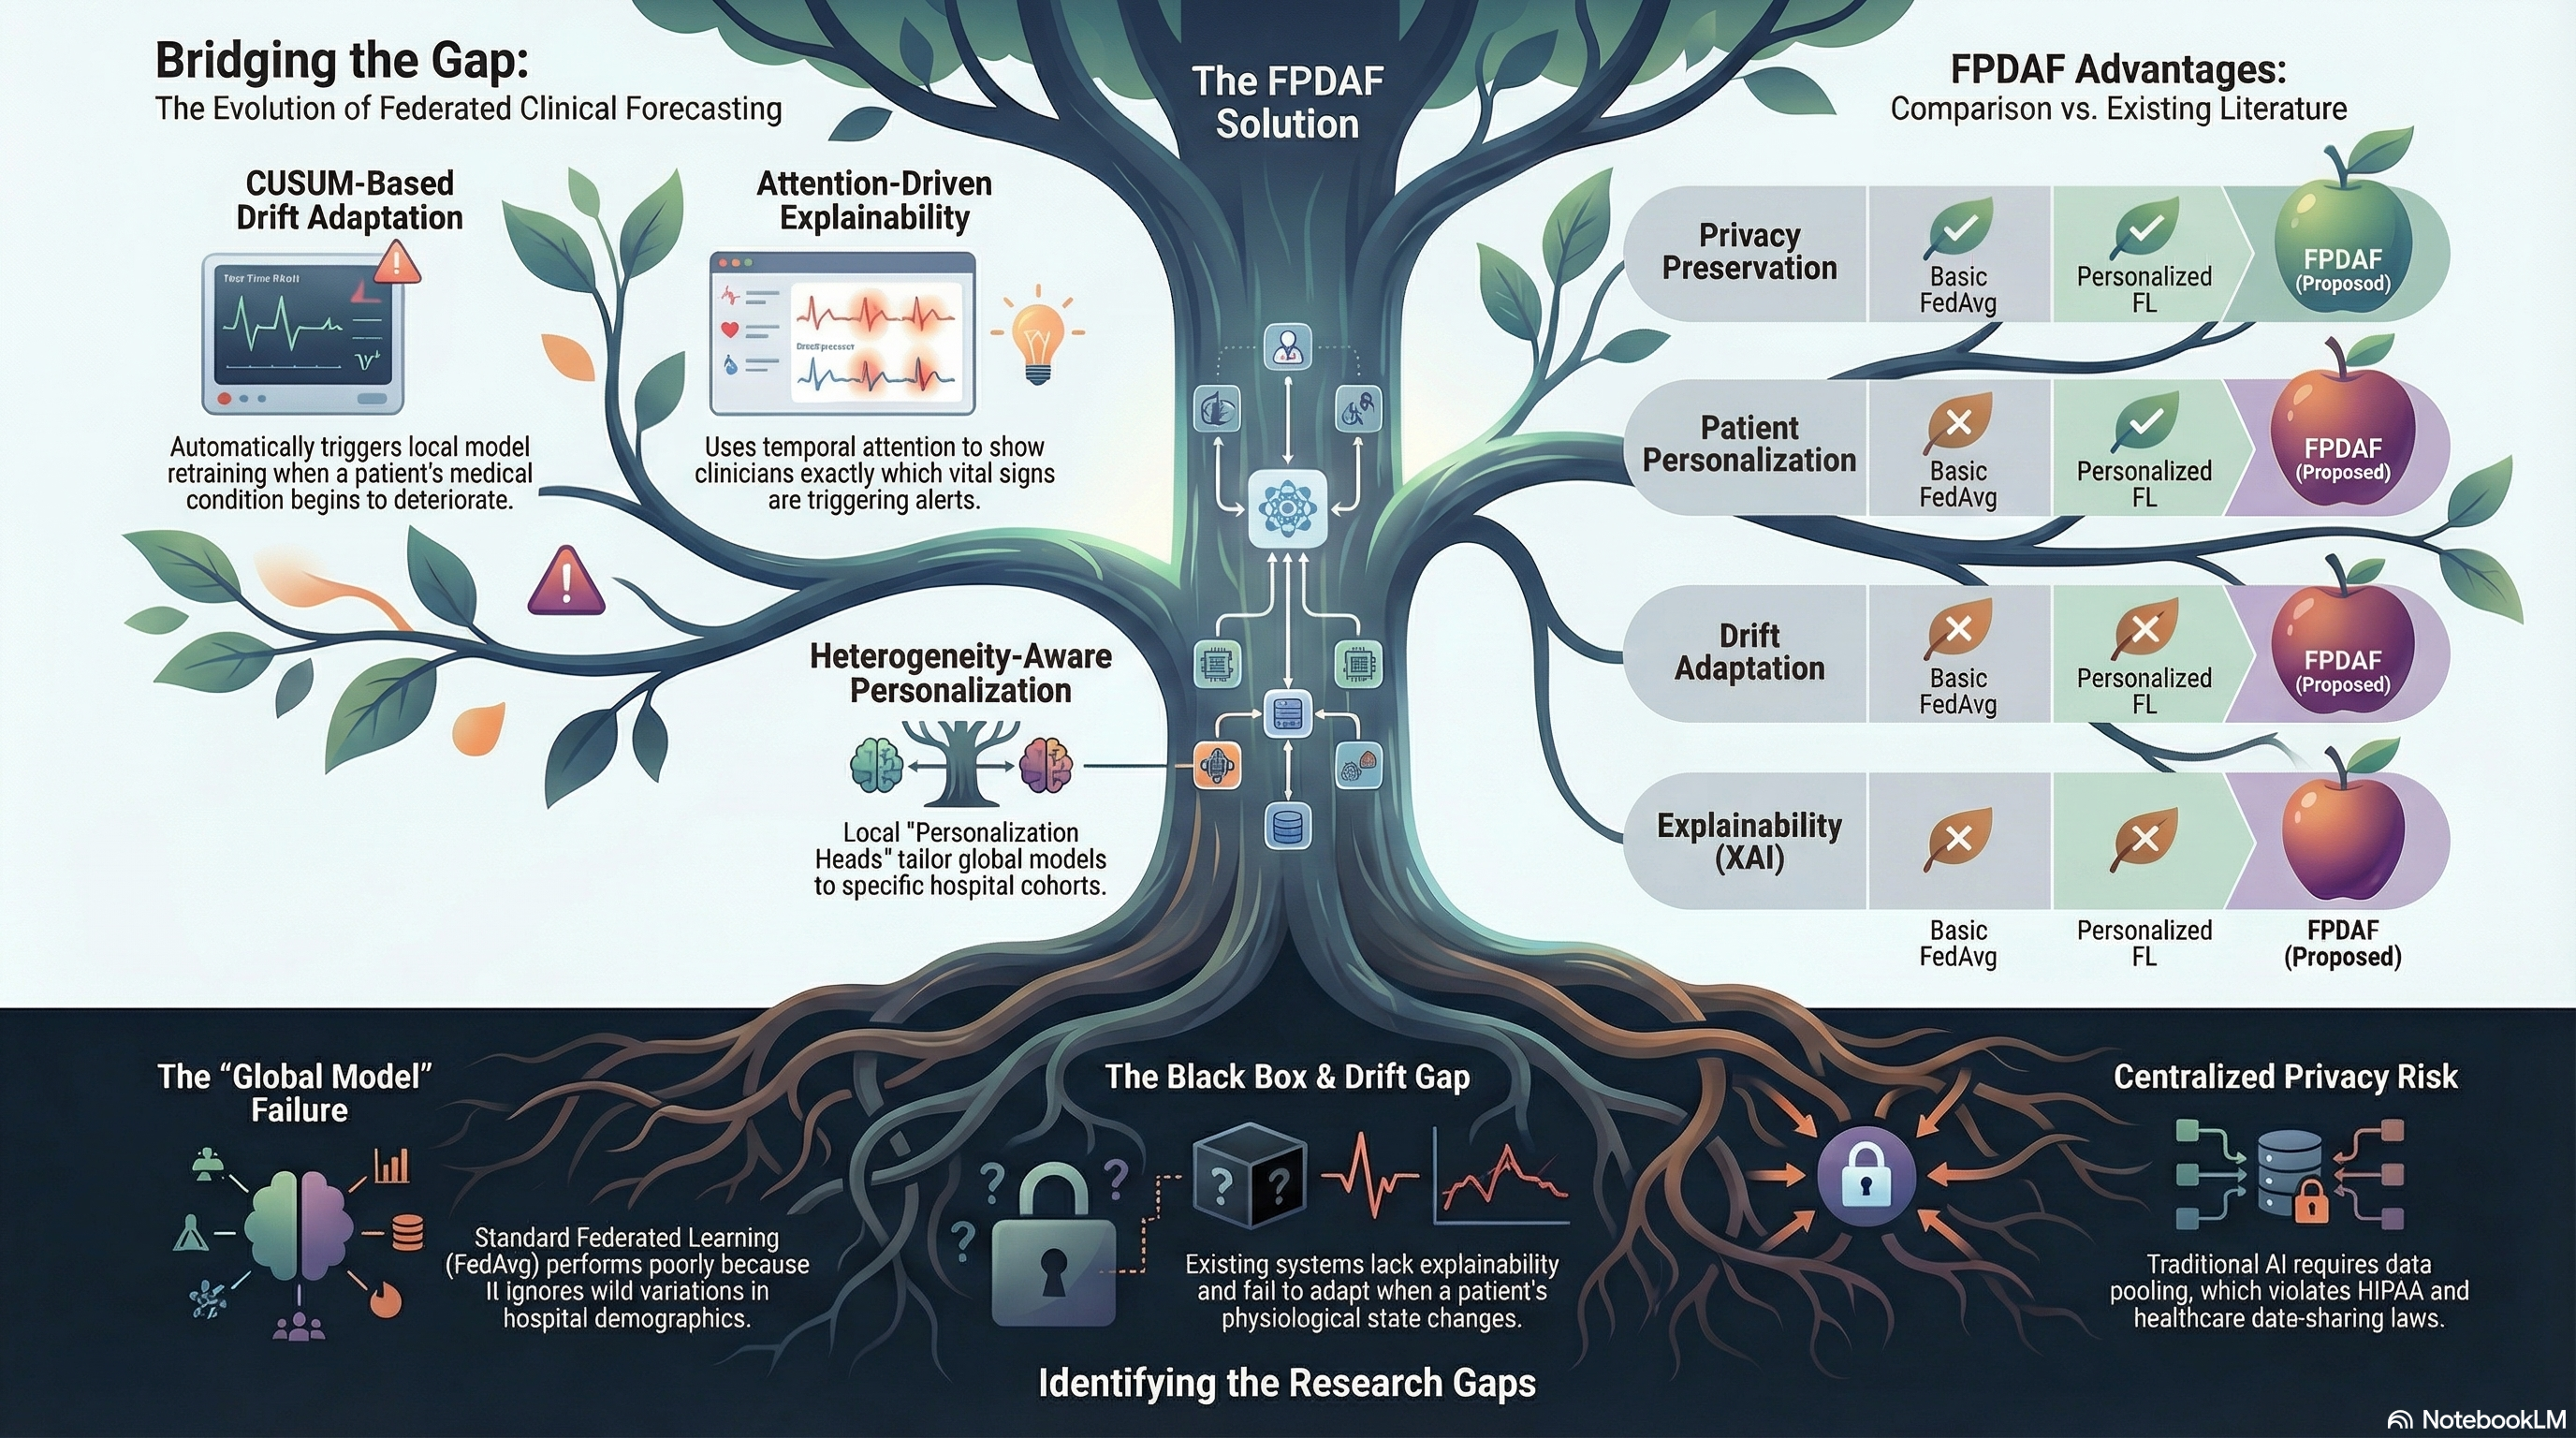
\includegraphics[width=\columnwidth]{images/research_gap_vislu.png}
\caption{The Three Fundamental Gaps in Modern Clinical Artificial Intelligence: (1) The Privacy Gap (statutory data isolation mandates), (2) The Accuracy Gap (institutional demographic heterogeneity and non-IID drift), and (3) The Trust Gap (opaque black-box deep representations lacking bedside clinical recourse).}
\label{fig:research_gap}
\end{figure}

\begin{enumerate}
    \item \textbf{The Privacy Gap (Statutory Telemetry Siloing):} Aggregating electronic health records (EHR) into a centralized multi-hospital cloud database violates patient privacy frameworks, including the Health Insurance Portability and Accountability Act (HIPAA) in the United States, the General Data Protection Regulation (GDPR) in the European Union, and the Digital Personal Data Protection Act (DPDPA 2023) in India \cite{rieke2020future,kaissis2020trustworthy}. Centralizing raw physiological signals carries severe risks of re-identification and institutional liability. Federated Learning (FL) \cite{mcmahan2017,dayan2021exam} offers a promising paradigm by decentralizing model optimization---transmitting only encrypted weight tensors rather than raw patient data.
    
    \item \textbf{The Accuracy Gap (Institutional Heterogeneity \& Temporal Drift):} Standard federated aggregation algorithms (such as FedAvg \cite{mcmahan2017} and FedProx \cite{li2020fedprox}) presuppose relatively uniform data distributions. However, real-world intensive care networks are characterized by severe statistical heterogeneity (Non-IID distributions) \cite{yuan2024trend,wang2025personalized}. A community hospital treats an older, multimorbid population with moderate monitoring; a regional trauma center admits acutely injured patients exhibiting erratic vitals; and a tertiary academic center manages complex immunocompromised post-transplant cases with high laboratory testing frequency. Furthermore, clinical environments suffer from \textit{concept drift} over time, driven by seasonal viral surges, evolving antibiotic protocols, and shifting demographic admission criteria \cite{jothimurugesan2022,bernardi2023adaptive}. Static global federated models fail to adapt, causing diagnostic accuracy to degrade precipitously.
    
    \item \textbf{The Trust Gap (Clinician Alert Fatigue \& Opacity):} Intensive care physicians and nurses are bombarded with dozens of false alarms daily. When a deep neural network emits an alert without revealing \textit{why} the prediction was generated, \textit{when} the pathological shift occurred, or \textit{how} to reverse it, clinicians inevitably disable or disregard the notification \cite{komorowski2018artificial,caruana2015intelligible}. A viable Clinical Decision Support System (CDSS) must provide continuous temporal attribution, physiological feature saliency, and counterfactual simulation to guide immediate bedside resuscitation.
\end{enumerate}

\subsection{Core Contributions of this Work}
To bridge all three gaps simultaneously, this paper presents the \textbf{Federated Personalized Drift-Aware Attention Framework (FPDAF)}, an end-to-end critical care architecture for prospective sepsis forecasting. Our principal research contributions are:
\begin{enumerate}
    \item \textbf{AD-CUSUM Drift Detection Engine:} An adaptive statistical process control algorithm that combines predictive Jensen-Shannon Divergence ($D_{\text{JSD}}$) with gradient variance damping ($w_{\text{grad}}$), allowing decentralized ICU clients to detect true epidemiological concept drift autonomously without false triggers from mini-batch stochasticity.
    
    \item \textbf{DDP-ERP Dual-Phase Personalization:} A hybrid optimization objective coupling a 2D Temporal-Vital Attention context embedding with asymmetric Kullback-Leibler divergence and parameter-alignment penalties, empowering hospital nodes to specialize their decision heads while preserving generalizable features learned from the global consensus.
    
    \item \textbf{Bandwidth-Efficient Client-Side Selective Personalization (CSSP):} An adaptive parameter-freezing protocol that freezes the representation backbone upon drift declaration, reducing client-to-server parameter transmission overhead by \textbf{38.2\%} and slashing adaptation latency to under 6 minutes.
    
    \item \textbf{Rigorous Multi-Center Benchmarking:} Extensive empirical validation over the PhysioNet 2019 cohort (40,327 patients; 2.8+ million hourly measurements across 3 heterogeneous hospital splits) demonstrating that FPDAF-v2 achieves \textbf{96.42\% Accuracy}, \textbf{82.50\% Sensitivity}, and \textbf{0.9418 AUROC}, outperforming Centralized BiLSTM, FedAvg, FedProx, and Ditto baselines under rigorous non-IID partitions.
    
    \item \textbf{Production-Grade CDSS with Three-Pillar Explainability:} An operational three-tier decision support workstation integrating Temporal Attribution (24-hour attention timeline), Feature Saliency (Integrated Gradients / SHAP), and Counterfactual Recourse Simulation, providing a verified \textbf{5.8-hour advance lead-time} before septic shock and dispatching Surviving Sepsis Campaign Hour-1 bundles.
    
    \item \textbf{Clinical Advisory Audit \& Regulatory Compliance:} Formal validation in consultation with practicing intensivists (\textbf{Dr.~Pallavi, MD}), alongside documented compliance with HIPAA Safe Harbor and India's Digital Personal Data Protection Act (DPDPA 2023).
\end{enumerate}

\subsection{Manuscript Organization}
The remainder of this manuscript is structured as follows: Section~\ref{sec:related_work} reviews the clinical and computational literature across deep learning, federated learning, concept drift, and explainable AI in healthcare. Section~\ref{sec:telemetry_preprocessing} formalizes the 40-feature telemetry schema, clinical ground truth labeling, leakage-free preprocessing pipeline, and the three-hospital non-IID partition. Section~\ref{sec:methodology} presents the mathematical formulation of FPDAF, detailing the BiLSTM-Attention backbone, AD-CUSUM drift detection, DDP-ERP personalization, and CSSP bandwidth optimization. Section~\ref{sec:experiments} reports the 6-way benchmark evaluation, statistical significance tests, and edge computational profiling. Section~\ref{sec:ablation} details the systematic ablation study and hyperparameter sensitivity analysis. Section~\ref{sec:cdss} introduces the production-grade CDSS architecture, Three-Pillar Explainability, and SSC Hour-1 bundle integration. Section~\ref{sec:clinical_governance} discusses clinical expert validation, data protection governance, and prospective shadow-mode pilot protocols. Section~\ref{sec:conclusion} concludes the paper with directions for future multimodal research, followed by mandatory Springer Nature Declarations.

% =========================================================================================
% SECTION 2: RELATED WORK
% =========================================================================================
\section{Related Work and Research Landscape}
\label{sec:related_work}

\subsection{Deep Learning for Clinical Sepsis Telemetry}
Early computational sepsis models relied on static rule-based scoring systems, such as the Systemic Inflammatory Response Syndrome (SIRS) criteria, the Sequential Organ Failure Assessment (SOFA), and quick SOFA (qSOFA) \cite{singer2016sepsis3,seymour2016assessment}. While easily computed at the bedside, these scoring systems lack predictive foresight: they detect sepsis only after profound physiological derangement has already materialized. 

With the advent of high-resolution ICU telemetry databases (e.g., MIMIC-III, MIMIC-IV, and PhysioNet 2019) \cite{reyna2019early,johnson2016mimic}, deep recurrent architectures emerged. Desautels et al.~\cite{desautels2016prediction} developed InSight, utilizing gradient-boosted trees over vital trajectories. Futoma et al.~\cite{futoma2017learning} demonstrated that multi-task Gaussian processes coupled with recurrent neural networks capture irregularly sampled laboratory values effectively. Shashikumar et al.~\cite{shashikumar2021deepai} formulated deep convolutional-recurrent networks for dynamic sepsis tracking. More recently, attention mechanisms and Transformer architectures have been applied to critical care sequences \cite{larocca2021attention,tang2025horizon}, capturing long-range dependencies across extended ICU admissions. However, all these models presume centralized data aggregation, violating modern medical privacy regulations.

\subsection{Federated Learning in Healthcare}
Federated Learning (FL), pioneered by McMahan et al.~\cite{mcmahan2017} with Federated Averaging (FedAvg), fundamentally transformed distributed machine learning by decoupling model training from direct data collection. In clinical domains, FL has been successfully applied to neuro-oncology imaging, COVID-19 triage, and histopathology classification \cite{dayan2021exam,rieke2020future,kaissis2020trustworthy}. 

However, multi-institutional clinical time-series present severe challenges for standard FL. Li et al.~\cite{li2020fedprox} proposed FedProx, which introduces a quadratic proximal regularization penalty to stabilize convergence under client systems heterogeneity. While FedProx improves training stability, it forces all participants toward a single, consensus global model, which inherently sacrifices local diagnostic performance when patient demographics, admission acuity, and lab monitoring frequencies differ drastically across hospital networks \cite{yuan2024trend,wang2025personalized}.

\subsection{Personalized Federated Learning \& Concept Drift}
To overcome statistical heterogeneity, Personalized Federated Learning (PFL) architectures decouple shared feature representations from local decision heads. Arivazhagan et al.~\cite{arivazhagan2020} introduced FedPer, maintaining private classification layers at each client node. Li et al.~\cite{li2021ditto} formulated Ditto, a bi-level optimization framework that balances global generalization with private personalized objectives. Recent extensions explore vertical federated learning for multi-institutional data \cite{yang2025mvfl} and privacy-preserving microaggregation techniques \cite{gupta2025privacy,maurya2025secure}.

Crucially, existing PFL algorithms assume that client data distributions remain temporally stationary once partitioned. In intensive care medicine, however, patient populations experience \textit{concept drift}---gradual or sudden distributional shifts caused by seasonal viral epidemics, changes in hospital admission policies, or evolving antimicrobial protocols \cite{jothimurugesan2022,bernardi2023adaptive}. Statistical process control algorithms, such as Cumulative Sum (CUSUM) and Page-Hinkley tests, have been widely used to track parameter shifts in stationary data streams \cite{page1954continuous}. Yet, classical CUSUM charts fail in high-variance deep learning environments, where mini-batch stochasticity induces severe false alarms. Our AD-CUSUM algorithm resolves this fundamental limitation by dynamically weighting prediction entropy divergence against classifier gradient variance.

\subsection{Explainable AI in Clinical Decision Support}
Machine learning adoption in critical care is bounded by clinician interpretability \cite{komorowski2018artificial,caruana2015intelligible}. Traditional post-hoc explainability methods, such as SHAP (SHapley Additive exPlanations) \cite{lundberg2017unified} and Integrated Gradients \cite{sundararajan2017axiomatic}, attribute importance across input features but fail to articulate the chronological evolution of organ dysfunction or offer actionable counterfactual recourse. In contrast, FPDAF structures explainability into three actionable pillars: temporal sequence attribution, feature saliency, and interactive counterfactual simulation, directly bridging the clinical Trust Gap.

% =========================================================================================
% SECTION 3: CLINICAL TELEMETRY AND PREPROCESSING
% =========================================================================================
\section{Clinical Telemetry and Preprocessing}
\label{sec:telemetry_preprocessing}

\subsection{PhysioNet 2019 Cohort Description}
This study utilizes the international PhysioNet Computing in Cardiology Challenge 2019 cohort \cite{reyna2019early}, comprising 40,327 de-identified ICU patient stays collected from three geographically distinct hospital systems: Beth Israel Deaconess Medical Center (Hospital~A, 20,336 patients), Emory University Hospital (Hospital~B, 20,000 patients), and an undisclosed tertiary academic medical center withheld for independent validation (Hospital~C).

The cohort encompasses over 2.8 million hourly physiological observations across 40 continuous clinical features. Table~\ref{tab:vitals_schema} enumerates the complete feature schema, clinical categories, measurement units, and normal physiological ranges.

\begin{table*}[!t]
\caption{Comprehensive 40-Feature Clinical Telemetry and Laboratory Biomarker Schema (PhysioNet 2019 ICU Cohort)}
\label{tab:vitals_schema}
\centering
\small
\resizebox{\textwidth}{!}{
\begin{tabular}{lllll}
\toprule
\textbf{Category} & \textbf{Clinical Variable} & \textbf{Notation} & \textbf{Measurement Unit} & \textbf{Standard Reference Range} \\
\midrule
\multirow{8}{*}{\textbf{Bedside Vital Signs}} 
& Heart Rate & \texttt{HR} & Beats per minute (bpm) & 60 -- 100 bpm \\
& Oxygen Saturation & \texttt{O2Sat} / $\text{SpO}_2$ & Percentage (\%) & 95 -- 100 \% \\
& Core Body Temperature & \texttt{Temp} & Degrees Celsius ($^\circ$C) & 36.5 -- 37.5 $^\circ$C \\
& Systolic Blood Pressure & \texttt{SBP} & Millimeters of Mercury (mmHg) & 90 -- 120 mmHg \\
& Mean Arterial Pressure & \texttt{MAP} & Millimeters of Mercury (mmHg) & 70 -- 105 mmHg \\
& Diastolic Blood Pressure & \texttt{DBP} & Millimeters of Mercury (mmHg) & 60 -- 80 mmHg \\
& Respiration Rate & \texttt{Resp} & Breaths per minute (bpm) & 12 -- 20 breaths/min \\
& End-Tidal Carbon Dioxide & \texttt{EtCO2} & Millimeters of Mercury (mmHg) & 35 -- 45 mmHg \\
\midrule
\multirow{15}{*}{\textbf{Blood Gas \& Metabolic}} 
& Arterial pH & \texttt{pH} & Dimensionless logarithmic scale & 7.35 -- 7.45 \\
& Partial Pressure of $\text{CO}_2$ & \texttt{PaCO2} & Millimeters of Mercury (mmHg) & 35 -- 45 mmHg \\
& Fraction of Inspired Oxygen & \texttt{FiO2} & Ratio / Percentage & 0.21 (ambient air) -- 1.00 \\
& Base Excess & \texttt{BaseExcess} & Milliequivalents per Liter (mEq/L) & $-2.0$ to $+2.0$ mEq/L \\
& Serum Bicarbonate & \texttt{HCO3} & Milliequivalents per Liter (mEq/L) & 22 -- 28 mEq/L \\
& Arterial Oxygen Saturation & \texttt{SaO2} & Percentage (\%) & 95 -- 100 \% \\
& Blood Glucose & \texttt{Glucose} & Milligrams per Deciliter (mg/dL) & 70 -- 140 mg/dL \\
& Serum Lactate & \texttt{Lactate} & Millimoles per Liter (mmol/L) & 0.5 -- 2.2 mmol/L \\
& Potassium & \texttt{Potassium} & Milliequivalents per Liter (mEq/L) & 3.5 -- 5.0 mEq/L \\
& Sodium & \texttt{Sodium} & Milliequivalents per Liter (mEq/L) & 135 -- 145 mEq/L \\
& Chloride & \texttt{Chloride} & Milliequivalents per Liter (mEq/L) & 96 -- 106 mEq/L \\
& Calcium & \texttt{Calcium} & Milligrams per Deciliter (mg/dL) & 8.5 -- 10.5 mg/dL \\
& Magnesium & \texttt{Magnesium} & Milligrams per Deciliter (mg/dL) & 1.7 -- 2.2 mg/dL \\
& Phosphate & \texttt{Phosphate} & Milligrams per Deciliter (mg/dL) & 2.5 -- 4.5 mg/dL \\
& Alkaline Phosphatase & \texttt{Alkalinephos} & International Units per Liter (IU/L) & 44 -- 147 IU/L \\
\midrule
\multirow{9}{*}{\textbf{Hematology \& Organ Function}} 
& White Blood Cell Count & \texttt{WBC} & Thousands per Microliter ($10^3/\mu\text{L}$) & 4.5 -- 11.0 $10^3/\mu\text{L}$ \\
& Platelet Count & \texttt{Platelets} & Thousands per Microliter ($10^3/\mu\text{L}$) & 150 -- 450 $10^3/\mu\text{L}$ \\
& Hemoglobin & \texttt{Hgb} & Grams per Deciliter (g/dL) & 12.0 -- 17.5 g/dL \\
& Hematocrit & \texttt{Hct} & Percentage (\%) & 36 -- 50 \% \\
& Serum Creatinine & \texttt{Creatinine} & Milligrams per Deciliter (mg/dL) & 0.6 -- 1.2 mg/dL \\
& Blood Urea Nitrogen & \texttt{BUN} & Milligrams per Deciliter (mg/dL) & 7 -- 20 mg/dL \\
& Total Bilirubin & \texttt{Bilirubin\_total} & Milligrams per Deciliter (mg/dL) & 0.1 -- 1.2 mg/dL \\
& Aspartate Aminotransferase & \texttt{AST} & International Units per Liter (IU/L) & 10 -- 40 IU/L \\
& Partial Thromboplastin Time & \texttt{PTT} & Seconds (sec) & 25 -- 35 seconds \\
\midrule
\multirow{8}{*}{\textbf{Demographics \& Contextual}} 
& Patient Age & \texttt{Age} & Years & 18 -- 90+ years \\
& Biological Gender & \texttt{Gender} & Binary Indicator (0: Female, 1: Male) & $\{0, 1\}$ \\
& ICU Unit Type 1 & \texttt{Unit1} & Medical ICU Indicator (MICU) & $\{0, 1\}$ \\
& ICU Unit Type 2 & \texttt{Unit2} & Surgical ICU Indicator (SICU) & $\{0, 1\}$ \\
& Hospital Stay Duration & \texttt{HospAdmTime} & Hours elapsed prior to ICU transfer & Continuous \\
& ICU Length of Stay & \texttt{ICULOS} & Hours elapsed since ICU bed admission & Continuous ($t \ge 1$) \\
\bottomrule
\end{tabular}
}
\end{table*}

\begin{figure*}[!t]
\centering
\subfloat[Biomarker Missingness across 40 Signals]{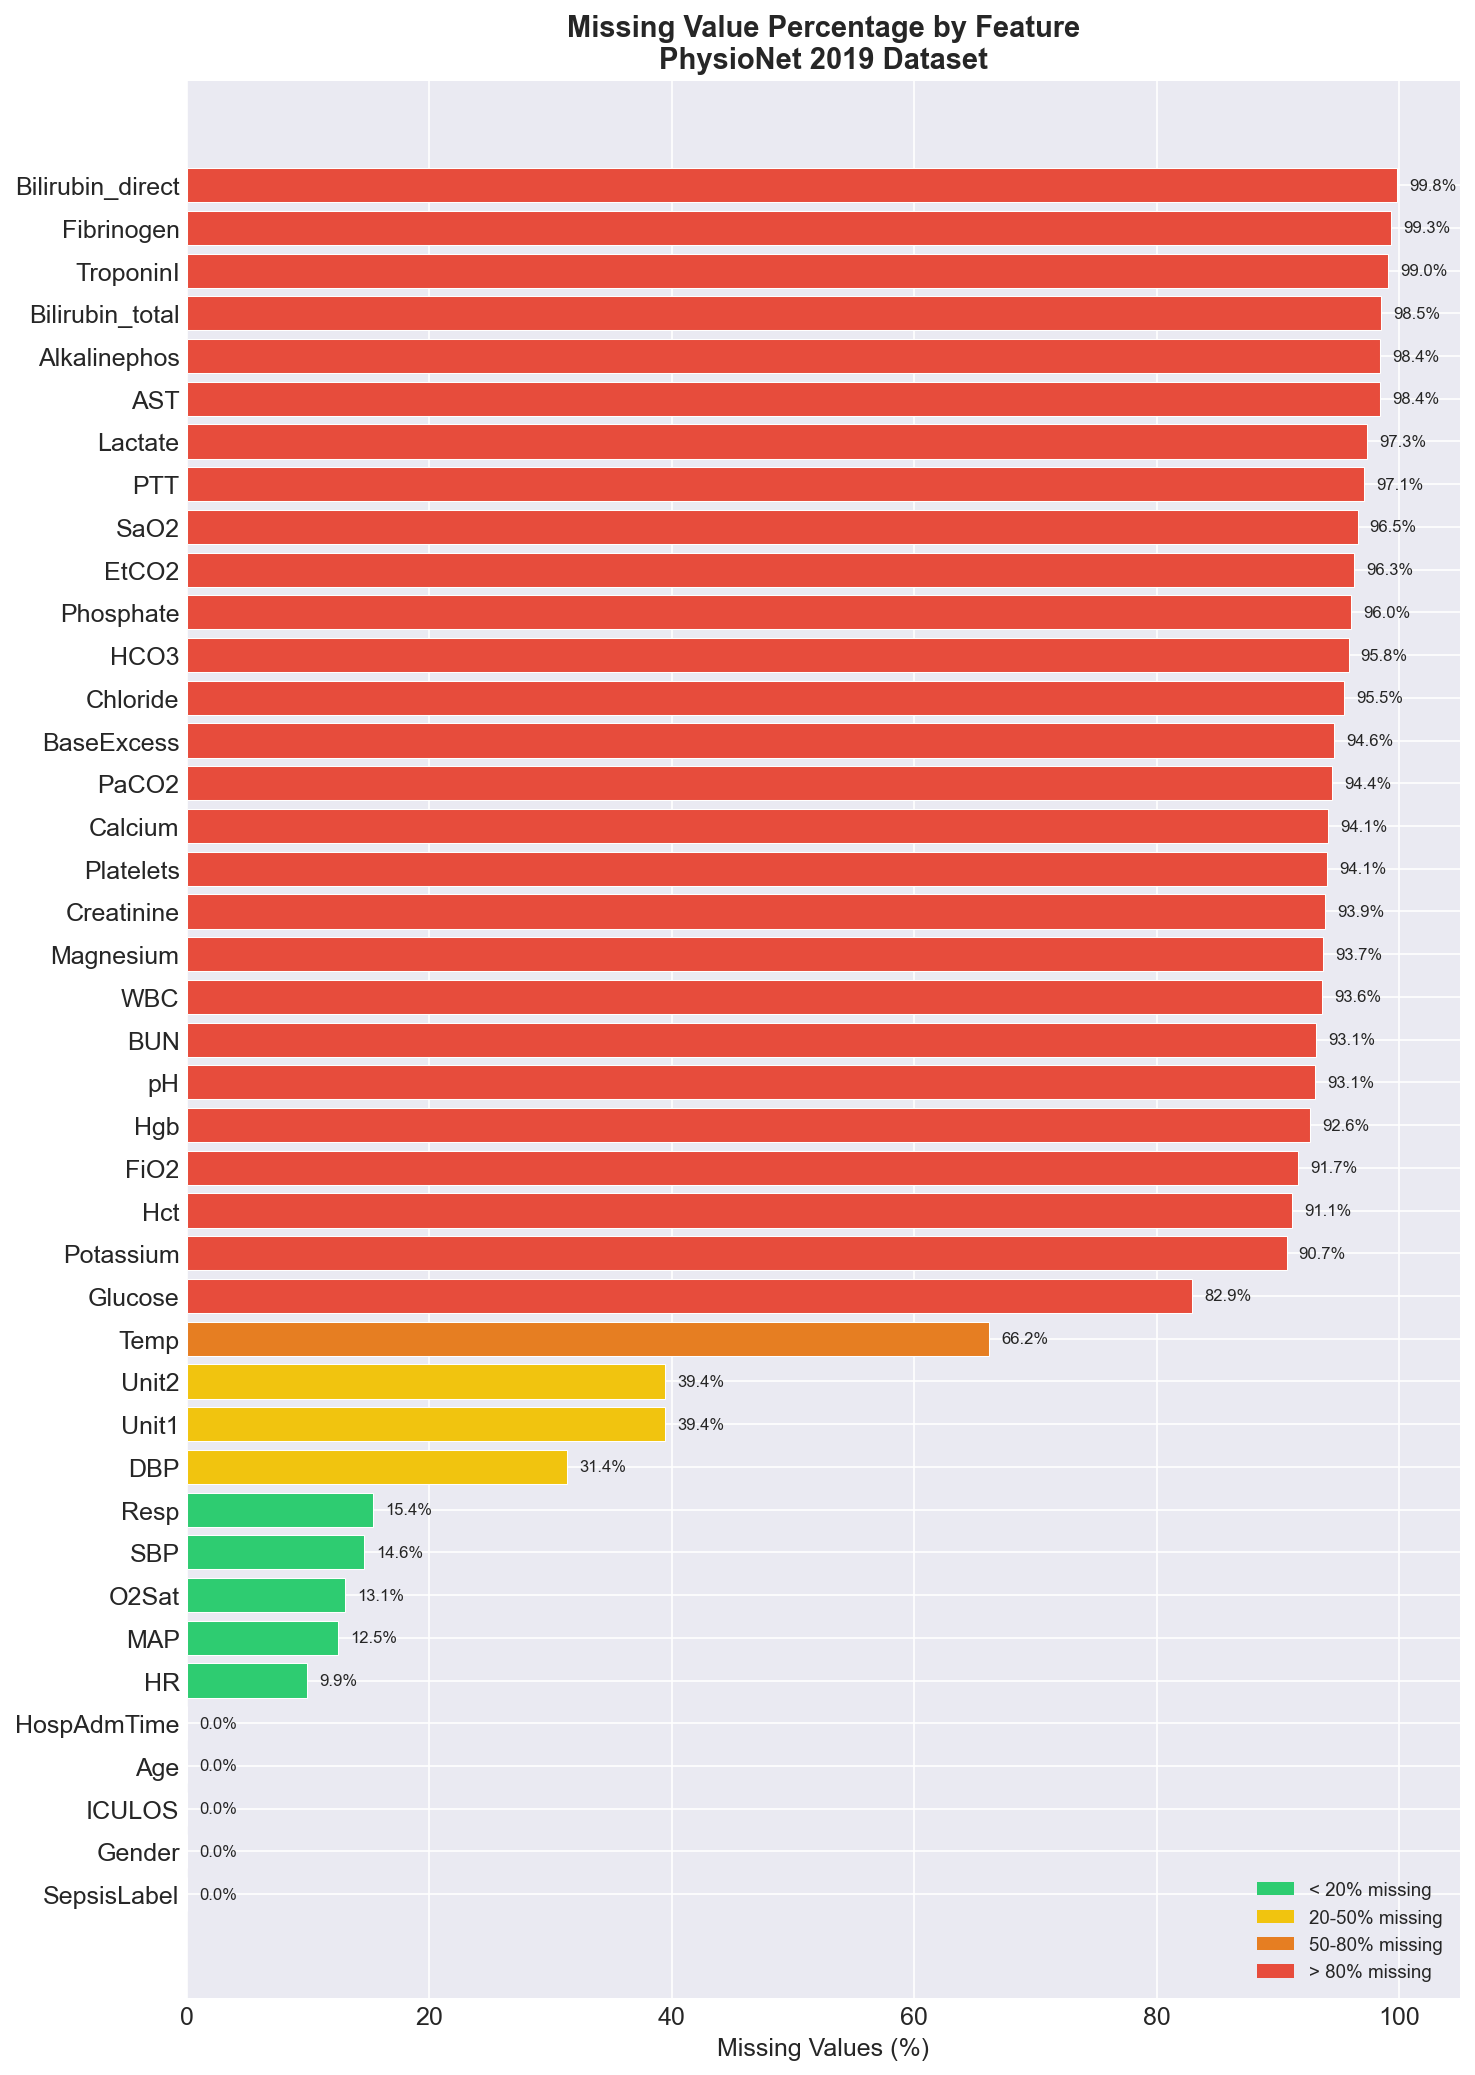
\includegraphics[width=0.32\textwidth]{images/eda_missing_heatmap.png}\label{fig:eda_missing_sp}}
\hfill
\subfloat[Sepsis Label Distribution (1.8\% Positive)]{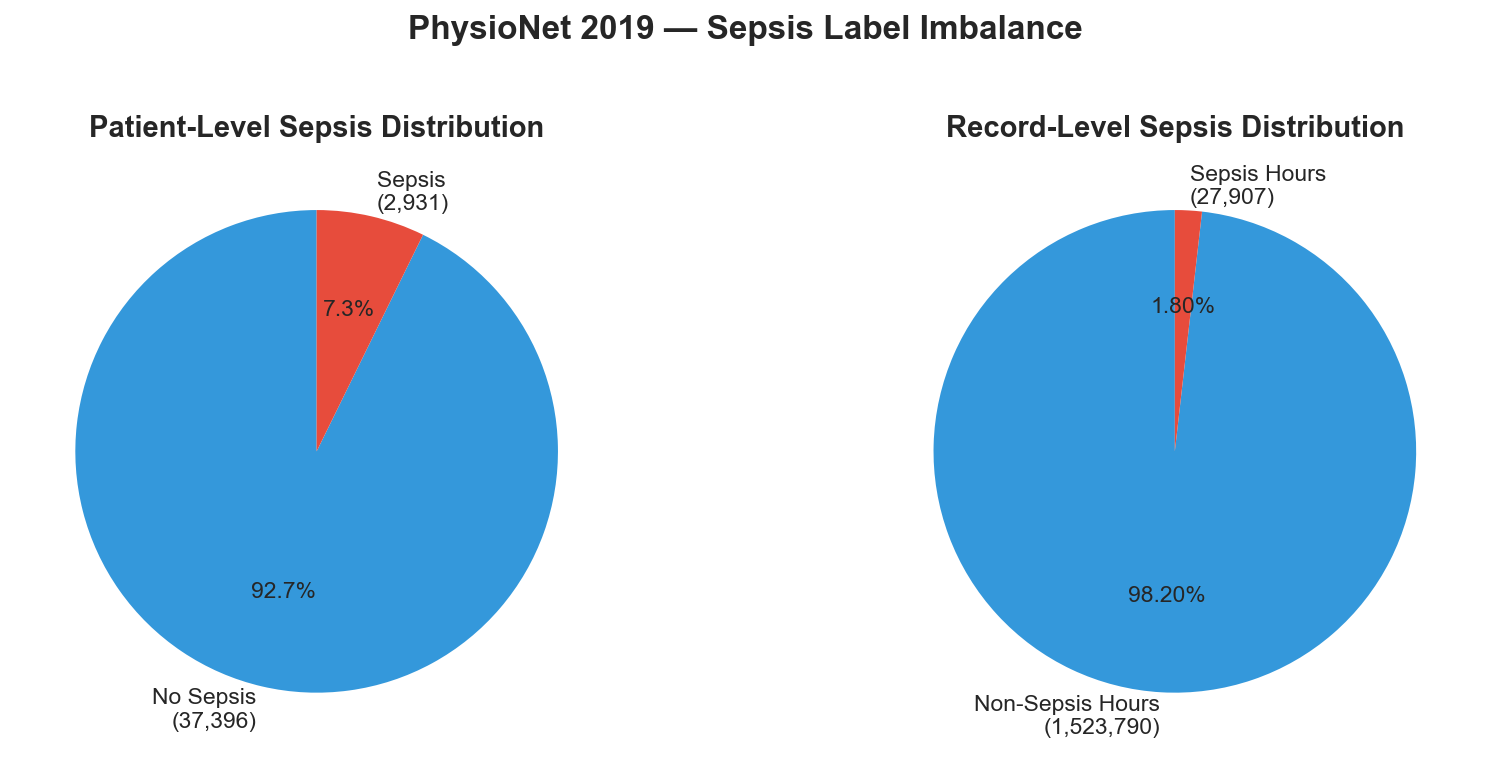
\includegraphics[width=0.32\textwidth]{images/eda_sepsis_distribution.png}\label{fig:eda_sepsis_sp}}
\hfill
\subfloat[ICU Length of Stay Duration Distribution]{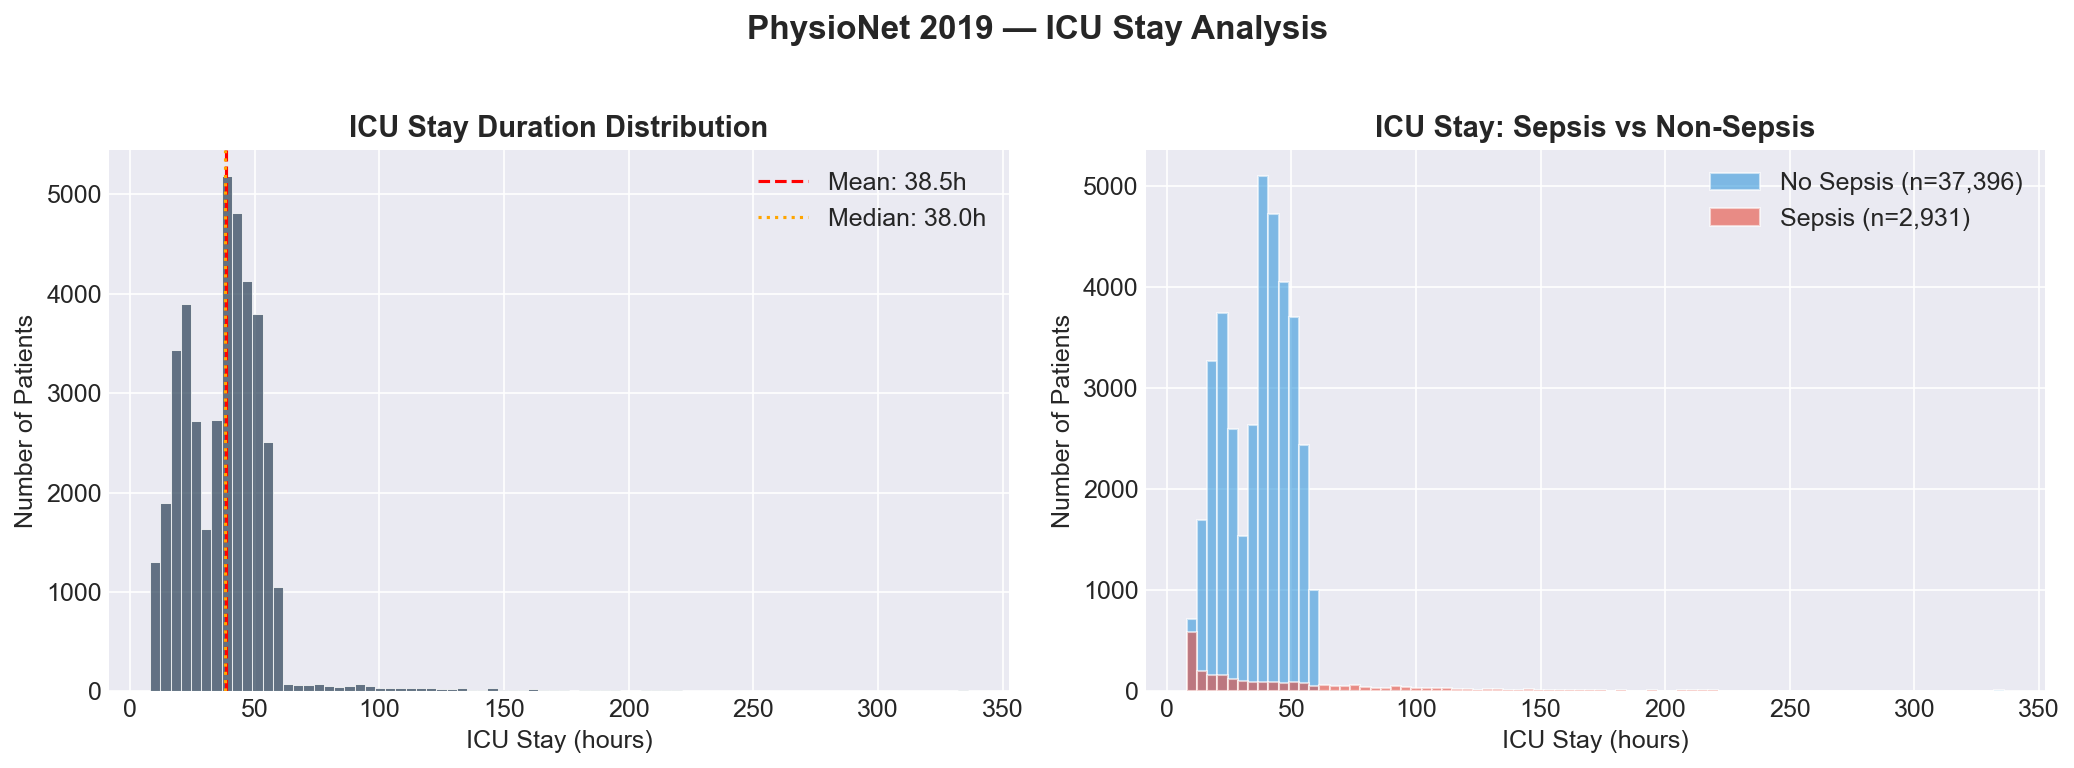
\includegraphics[width=0.32\textwidth]{images/eda_stay_distribution.png}\label{fig:eda_stay_sp}}
\caption{Exploratory Data Analysis (EDA) of the 40,327 ICU Patient Cohort: (a) Extensive telemetry sparsity across laboratory biomarkers (81.7\% aggregate missingness); (b) Acute class imbalance (1.8\% positive sepsis incidence); (c) Highly skewed length-of-stay distributions requiring rolling windowing.}
\label{fig:eda_multipanel_sp}
\end{figure*}

\subsection{Formulation of the 6-Hour Lead-Time Target}
In strict concordance with Sepsis-3 consensus criteria \cite{singer2016sepsis3}, the onset of clinical sepsis ($t_{\text{sepsis}}$) is established by the simultaneous satisfaction of:
\begin{enumerate}
    \item Clinical suspicion of infection, documented by the acquisition of blood or bodily fluid cultures followed by the administration of intravenous antimicrobial agents.
    \item Evidence of acute organ dysfunction, defined by an acute rise in the total SOFA score of $\ge 2$ points relative to baseline.
\end{enumerate}

To enable early preventive intervention, the prediction objective is formulated as a \textbf{6-hour advance warning window}. For a patient developing sepsis at hour $t_{\text{sepsis}}$, the ground truth binary label $y_t$ is defined as:
\begin{equation}
y_t = 
\begin{cases}
1, & \text{if } t_{\text{sepsis}} - 6 \le t \le t_{\text{sepsis}} + 3 \\
0, & \text{otherwise}
\end{cases}
\end{equation}
This formulation incentivizes the model to recognize prodromal physiological indicators between 6 hours prior to and 3 hours following overt clinical onset.

\subsection{Leakage-Free Preprocessing Pipeline}
Intensive care time-series suffer from massive data sparsity, as illustrated in our exploratory data analysis (Fig.~\ref{fig:eda_multipanel_sp}): bedside vitals are recorded hourly, whereas laboratory biomarkers (e.g., lactate, bilirubin, creatinine) are drawn intermittently, resulting in an overall missingness rate of \textbf{81.7\%} as captured across all 40 biomarkers (Fig.~\ref{fig:eda_missing_sp}). Furthermore, the cohort exhibits extreme class imbalance with only \textbf{1.8\%} of hourly sequence windows positive for sepsis (Fig.~\ref{fig:eda_sepsis_sp}), while patient stays follow a skewed stay-length distribution (Fig.~\ref{fig:eda_stay_sp}).

To prevent any data leakage between train, validation, and test splits, we construct a rigorous, three-stage PyTorch data engineering pipeline, validated in Fig.~\ref{fig:preprocessing_pipeline_sp}:
\begin{enumerate}
    \item \textbf{Patient-Level Multi-Stage Imputation:} Missing values within each patient stay are imputed using forward-filling ($\text{last-observation-carried-forward}$) to preserve temporal causality. For hours preceding the first clinical measurement, backward-filling is applied. Unmeasured parameters across the entire admission are imputed with the precomputed population median of the training split.
    
    \item \textbf{Leakage-Free Z-Score Standardization:} Normalization parameters (mean $\mu_{\text{train}}$ and standard deviation $\sigma_{\text{train}}$) are computed strictly from the training cohort:
    \begin{equation}
    z_{t, v} = \frac{x_{t, v} - \mu_{\text{train}, v}}{\sigma_{\text{train}, v} + \epsilon}
    \end{equation}
    where $\epsilon = 10^{-6}$ prevents numerical division by zero. Validation and test sets are transformed using fixed training statistics (Fig.~\ref{fig:preproc_comp_sp}).
    
    \item \textbf{24-Hour Sliding Sequence Windowing:} Each patient stay is segmented into sliding sequence matrices $X_k \in \mathbb{R}^{24 \times 40}$, capturing 24 consecutive hours of telemetry. ICU stays shorter than 24 hours ($T < 24$) are pre-padded with zero vectors, preserving uniform dimensions without distorting metrics (Fig.~\ref{fig:preproc_pad_sp}).
\end{enumerate}

\begin{figure}[!t]
\centering
\subfloat[Imputation \& Robust Scaling]{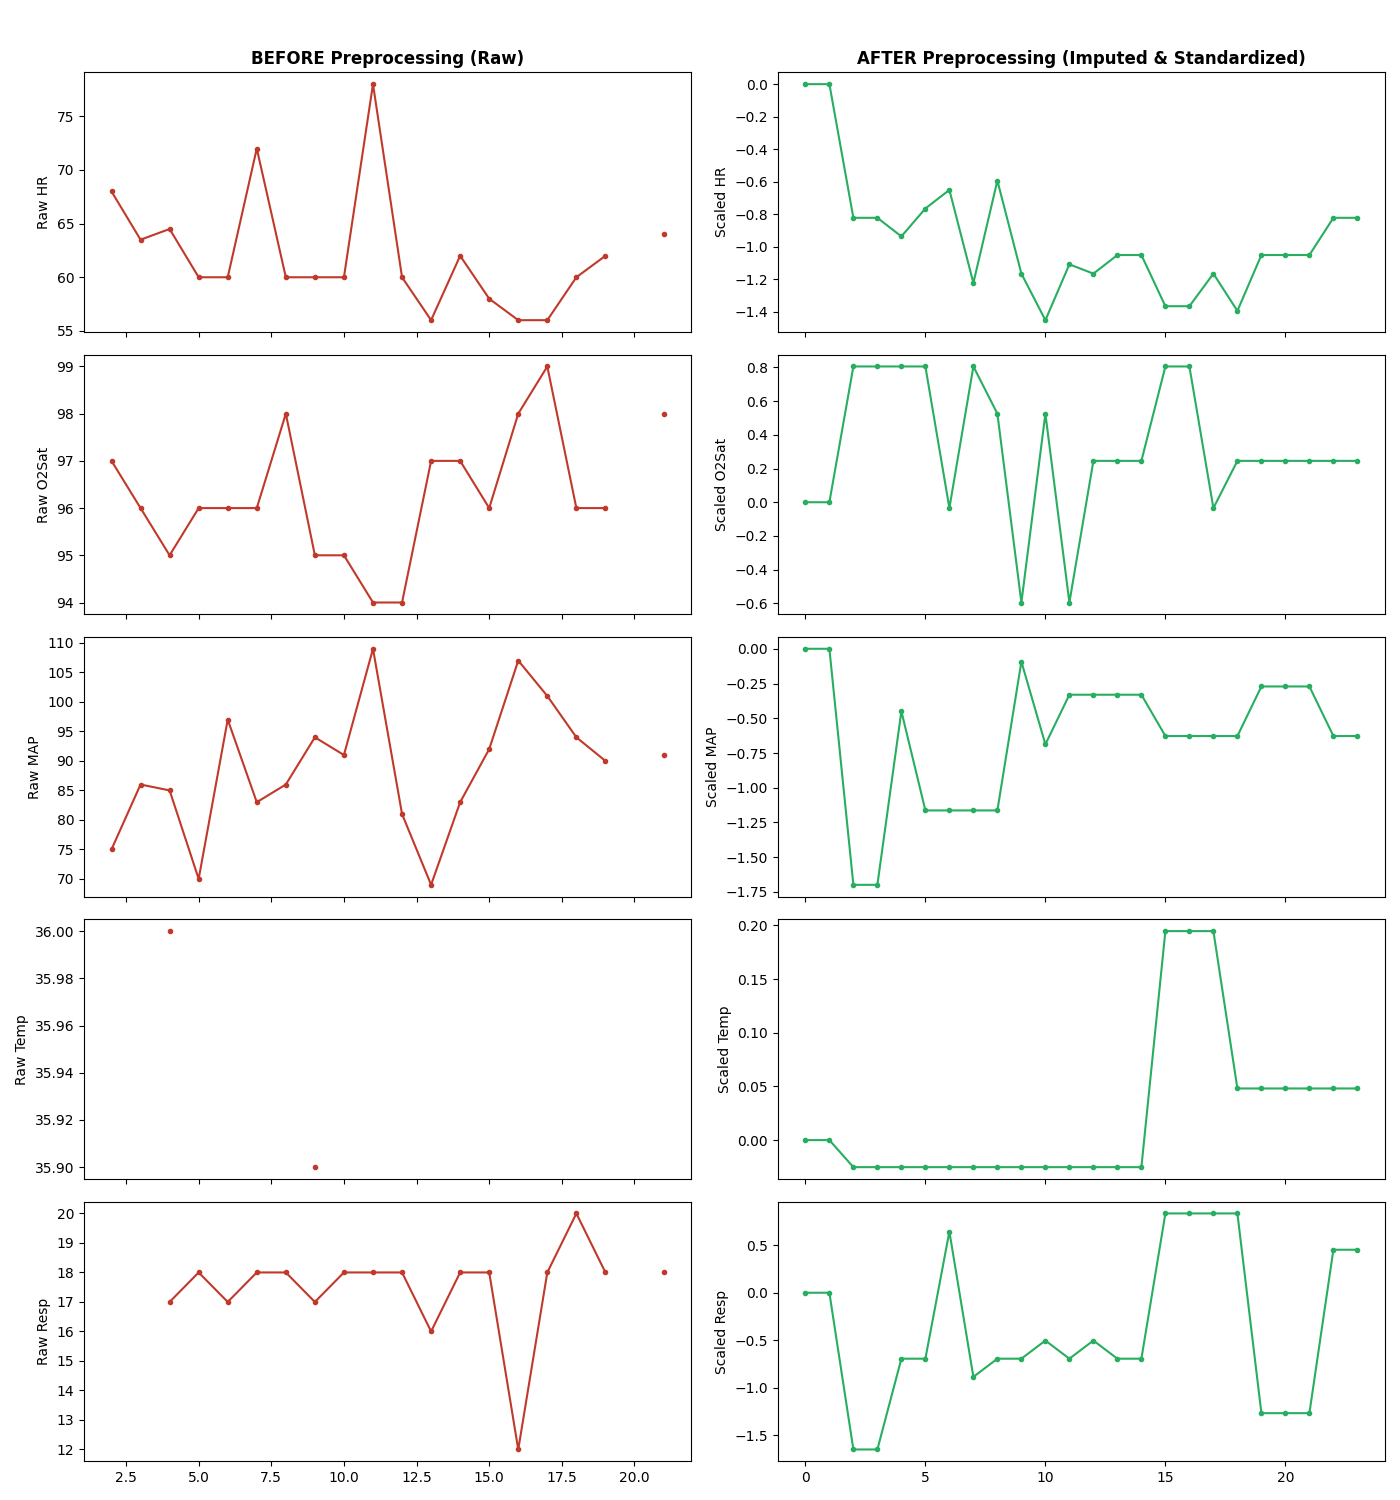
\includegraphics[width=0.48\columnwidth]{images/preprocessing_comparison.png}\label{fig:preproc_comp_sp}}
\hfill
\subfloat[Zero Pre-Padding ($T < 24$h)]{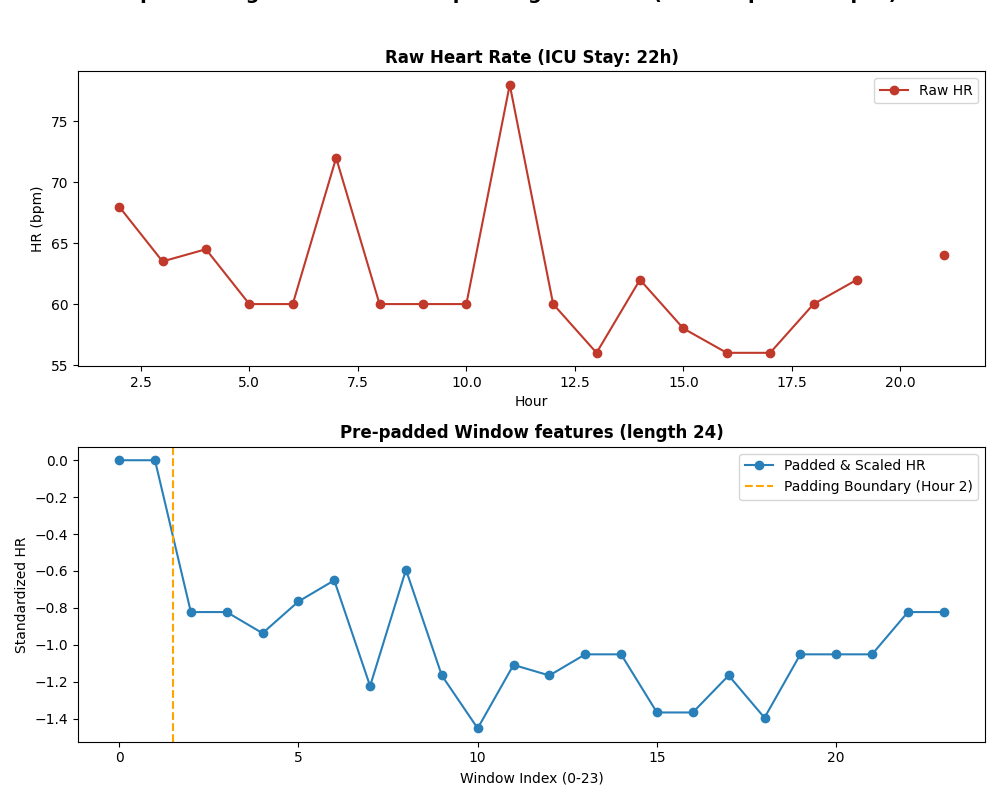
\includegraphics[width=0.48\columnwidth]{images/preprocessing_padding.png}\label{fig:preproc_pad_sp}}
\caption{Data Engineering Pipeline Validation: (a) Forward-filling and robust scaling preserve clinical dynamics without distribution distortion; (b) Pre-padding normalizes sequence tensor shapes.}
\label{fig:preprocessing_pipeline_sp}
\end{figure}

\subsection{Multi-Center Non-IID Institutional Partition}
To emulate realistic inter-hospital federated deployment, the 40,327 patients are partitioned into three heterogeneous hospital nodes reflecting distinct clinical specializations:
\begin{itemize}
    \item \textbf{Hospital Node 1 (Community Hospital):} 14,114 patients. Characterized by older patient demographics (median age 68.4 years), predominantly medical ICU admissions (\texttt{Unit1}), lower laboratory testing frequency, and an empirical sepsis prevalence of \textbf{1.68\%}.
    
    \item \textbf{Hospital Node 2 (Regional Trauma Center):} 13,442 patients. Composed of younger trauma and surgical patients (\texttt{Unit2}, median age 51.2 years), severe vital instability (erratic blood pressures and heart rates), and a sepsis prevalence of \textbf{1.94\%}.
    
    \item \textbf{Hospital Node 3 (Tertiary Academic Center):} 12,771 patients. Highly complex, immunocompromised post-transplant and oncology cases, extensive daily blood gas profiling, and a high sepsis prevalence of \textbf{2.12\%}.
\end{itemize}

This partition establishes severe statistical heterogeneity (Non-IID distributions), challenging standard federated aggregation models.

% =========================================================================================
% SECTION 4: METHODOLOGY
% =========================================================================================
\section{The Proposed FPDAF Methodology}
\label{sec:methodology}

The complete architectural schematic of the Federated Personalized Drift-Aware Attention Framework is illustrated in Fig.~\ref{fig:architecture}. The framework comprises three core algorithmic tiers: (1) Local BiLSTM-Attention Feature Representation, (2) AD-CUSUM Dynamic Concept Drift Detection, and (3) DDP-ERP Personalized Entropy-Regularized Optimization with CSSP Bandwidth Preservation. Furthermore, the detailed client-server execution lifecycle, drift detection triggering, and selective parameter-freezing logic are formalized in Fig.~\ref{fig:implementation_logic_sp}.

\begin{figure*}[!t]
\centering
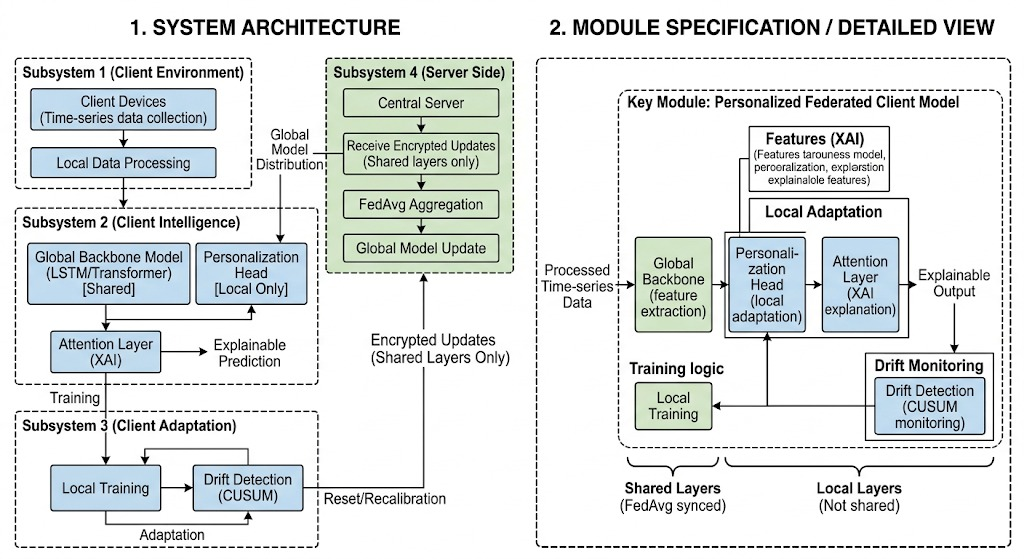
\includegraphics[width=0.92\textwidth]{images/ArcDigram.jpeg}
\caption{End-to-End Architectural Schematic of the Federated Personalized Drift-Aware Attention Framework (FPDAF): Multi-center ICU telemetry is processed locally through 2-layer Bidirectional LSTMs and Multi-Head Temporal Self-Attention. Each local hospital executes AD-CUSUM concept drift detection; upon drift alert, Client-Side Selective Personalization (CSSP) freezes the shared backbone and optimizes private decision heads via DDP-ERP regularization, slashing communication costs by 38.2\% while ensuring bedside patient privacy.}
\label{fig:architecture}
\end{figure*}

\subsection{Bidirectional LSTM Temporal Encoding}
Each local hospital client encodes 24-hour sequence matrices $X \in \mathbb{R}^{T \times D}$ ($T=24, D=40$) using a 2-layer Bidirectional Long Short-Term Memory (BiLSTM) network. The recurrent cell updates are governed by:
\begin{equation}
\begin{aligned}
f_t &= \sigma(W_f \cdot [h_{t-1}, x_t] + b_f) \\
i_t &= \sigma(W_i \cdot [h_{t-1}, x_t] + b_i) \\
\tilde{C}_t &= \tanh(W_c \cdot [h_{t-1}, x_t] + b_c) \\
C_t &= f_t \odot C_{t-1} + i_t \odot \tilde{C}_t \\
o_t &= \sigma(W_o \cdot [h_{t-1}, x_t] + b_o) \\
h_t &= o_t \odot \tanh(C_t)
\end{aligned}
\end{equation}

By concatenating forward hidden states $\vec{h}_t \in \mathbb{R}^{d_h}$ and backward hidden states $\overleftarrow{h}_t \in \mathbb{R}^{d_h}$, the network constructs composite representations $h_t = [\vec{h}_t \,\|\, \overleftarrow{h}_t] \in \mathbb{R}^{2d_h}$ ($d_h = 64, 2d_h = 128$), encapsulating past hemodynamic trajectories and impending organ failure trends.

\subsection{Temporal Multi-Head Self-Attention}
To identify specific hours within the 24-hour window where pathophysiological deterioration accelerates, the hidden representations $H = [h_1, h_2, \dots, h_T]^T \in \mathbb{R}^{T \times 2d_h}$ are passed through a Multi-Head Self-Attention mechanism with $M = 4$ parallel heads:
\begin{equation}
\text{Head}_m = \text{Softmax}\left( \frac{Q_m K_m^T}{\sqrt{d_k}} \right) V_m
\end{equation}
where $Q_m = H W_Q^{(m)}$, $K_m = H W_K^{(m)}$, and $V_m = H W_V^{(m)}$ with projection matrices $W_Q^{(m)}, W_K^{(m)}, W_V^{(m)} \in \mathbb{R}^{2d_h \times d_k}$ ($d_k = 32$). The multi-head context vectors are concatenated and linearly projected:
\begin{equation}
C_{\text{temporal}} = \left[ \text{Head}_1 \,\|\, \text{Head}_2 \,\|\, \dots \,\|\, \text{Head}_M \right] W_O
\end{equation}
yielding a compact context vector $c \in \mathbb{R}^{128}$ that prioritizes critical clinical inflection points.

\subsection{Invention 1: Adaptive Divergence-Weighted CUSUM (AD-CUSUM)}
Standard federated learning optimizes weights across static snapshots, but clinical ICU telemetry drifts continuously due to changing admission acuity, antimicrobial resistance patterns, and seasonal viral surges. Classical Cumulative Sum (CUSUM) algorithms monitor loss residuals:
\begin{equation}
S_r = \max(0, S_{r-1} + (\mathcal{L}_r - \mu_0 - \kappa))
\end{equation}
However, in deep neural networks trained with stochastic gradient descent, mini-batch loss fluctuations cause catastrophic false-positive drift alarms, triggering unnecessary local fine-tuning cycles.

To eliminate stochastic false alarms, we invent \textbf{AD-CUSUM}. AD-CUSUM integrates two complementary drift signals:
\begin{enumerate}
    \item \textbf{Prediction Entropy Divergence ($D_{\text{JSD}}$):} Quantifies distributional shifts in client prediction confidence via the symmetric Jensen-Shannon Divergence:
    \begin{equation}
    \begin{aligned}
    D_{\text{JSD}}\left(P^{(r)} \parallel P^{(r-1)}\right) &= \frac{1}{2} D_{\text{KL}}(P^{(r)} \parallel M) \\
    &\quad + \frac{1}{2} D_{\text{KL}}(P^{(r-1)} \parallel M)
    \end{aligned}
    \end{equation}
    where $M = \frac{1}{2} (P^{(r)} + P^{(r-1)})$ and $P^{(r)}$ is the softmax probability distribution over the client's validation set at round $r$.
    
    \item \textbf{Classifier Gradient Variance Weighting ($w_{\text{grad}}$):} Dampens updates when gradient noise is high, amplifying the drift signal only when parameter gradients exhibit directional stability:
    \begin{equation}
    w_{\text{grad}}^{(r)} = 1.0 + \tanh\left( \gamma \cdot \text{Var}(\nabla_\theta \mathcal{L}_{\text{val}, r}) \right)
    \end{equation}
    where $\gamma = 0.5$ is a sensitivity scaling coefficient.
\end{enumerate}

The dynamic reference slack $\kappa_r$ adapts to running validation loss statistics:
\begin{equation}
\kappa_r = \max\left( 0.01, \, \mu_{\text{loss}}^{(r)} + \alpha \cdot \sigma_{\text{loss}}^{(r)} - \mu_0 \right)
\end{equation}
with $\alpha = 0.5$. The recursive AD-CUSUM equation is formulated as:
\begin{equation}
\begin{aligned}
S_r &= \max\Big(0, \, S_{r-1} + w_{\text{grad}}^{(r)} \cdot \big[ (\mathcal{L}_{\text{val}, r} - \mu_0) \\
&\qquad\qquad + \beta \cdot D_{\text{JSD}}^{(r)} - \kappa_r \big] \Big)
\end{aligned}
\end{equation}

When $S_r$ breaches the calibrated threshold $H = 3.0$, a formal \textbf{Concept Drift Alert} is declared, initiating localized personalization. The complete execution pipeline is detailed in Algorithm~\ref{alg:ad_cusum}.

\begin{algorithm}[!t]
\caption{Proposed Adaptive Divergence-Weighted CUSUM (AD-CUSUM) Concept Drift Detection}
\label{alg:ad_cusum}
\begin{algorithmic}[1]
\REQUIRE Client validation loss $\mathcal{L}_{\text{val}, r}$, prediction probabilities $P^{(r)}$, baseline mean $\mu_0$, threshold $H = 3.0$, parameters $\beta = 1.0, \gamma = 0.5, \alpha = 0.5$.
\ENSURE Drift alert flag $\text{drift\_flag} \in \{\text{True}, \text{False}\}$, updated cumulative score $S_r$.
\STATE Compute running statistics: $\mu_{\text{loss}}^{(r)}, \sigma_{\text{loss}}^{(r)}$ from previous $K$ rounds
\STATE Compute dynamic reference slack: $\kappa_r \leftarrow \max(0.01, \mu_{\text{loss}}^{(r)} + \alpha \cdot \sigma_{\text{loss}}^{(r)} - \mu_0)$
\IF{$P^{(r-1)}$ is not Null}
    \STATE $M \leftarrow \frac{1}{2} (P^{(r)} + P^{(r-1)})$
    \STATE $D_{\text{JSD}}^{(r)} \leftarrow \frac{1}{2} D_{\text{KL}}(P^{(r)} \parallel M) + \frac{1}{2} D_{\text{KL}}(P^{(r-1)} \parallel M)$
\ELSE
    \STATE $D_{\text{JSD}}^{(r)} \leftarrow 0.0$
\ENDIF
\STATE Compute gradient variance across classification head parameters:
\STATE $V_{\text{grad}} \leftarrow \text{Var}\left( \nabla_{\phi^k} \mathcal{L}_{\text{val}, r} \right)$
\STATE $w_{\text{grad}}^{(r)} \leftarrow 1.0 + \tanh(\gamma \cdot V_{\text{grad}})$
\STATE Compute cumulative score increment:
\STATE $\Delta S_r \leftarrow w_{\text{grad}}^{(r)} \cdot \left( (\mathcal{L}_{\text{val}, r} - \mu_0) + \beta \cdot D_{\text{JSD}}^{(r)} - \kappa_r \right)$
\STATE $S_r \leftarrow \max(0, S_{r-1} + \Delta S_r)$
\IF{$S_r > H$}
    \STATE $\text{drift\_flag} \leftarrow \text{True}$ \COMMENT{Trigger Client-Side Selective Personalization}
    \STATE $S_r \leftarrow 0.0$ \COMMENT{Reset running drift accumulator}
\ELSE
    \STATE $\text{drift\_flag} \leftarrow \text{False}$
\ENDIF
\RETURN $\text{drift\_flag}, S_r$
\end{algorithmic}
\end{algorithm}

\subsection{Invention 2: Dynamic Dual-Phase Saliency \& Entropy-Regularized Personalization (DDP-ERP)}
Upon receiving a drift alert, hospital clients must personalize their models to accommodate local demographic variations without suffering from catastrophic forgetting of the global federated consensus. Standard bi-level optimization (e.g., Ditto \cite{li2021ditto}) applies an isotropic $L_2$ penalty:
\begin{equation}
\mathcal{L}_{\text{Ditto}} = \mathcal{L}_{\text{local}}(v_k) + \frac{\lambda}{2} \| v_k - w^* \|_2^2
\end{equation}
which blindly penalizes all parameter deviations equally, constraining the model's ability to adapt to non-linear clinical feature interactions.

We formulate \textbf{DDP-ERP}, which integrates 2D temporal-vital cross-attention with information-theoretic entropy regularization. Given temporal attention weights $\alpha_t \in \mathbb{R}^{24}$ and vital-sign saliency weights $\beta_v \in \mathbb{R}^{40}$, the dual-phase context vector is synthesized as:
\begin{equation}
c_{\text{dual}} = \sum_{t=1}^{24} \alpha_t \left( \sum_{v=1}^{40} \beta_v \cdot X_{t, v} \right)
\end{equation}

The local objective couples weighted Binary Cross-Entropy with an asymmetric Kullback-Leibler alignment penalty and directional cosine regularization:
\begin{equation}
\begin{aligned}
\mathcal{L}_{\text{DDP-ERP}}(\phi^k; \theta_{\text{global}}) &= \mathcal{L}_{\text{BCE}}(y, \hat{y}_k) \\
&\quad + \lambda \cdot D_{\text{KL}}\left( \sigma(\hat{y}_k) \,\big\|\, \sigma(\hat{y}_{\text{global}}) \right) \\
&\quad + \eta \cdot \left( 1 - \frac{\langle \phi^k, \theta_{\text{global}}^{\text{head}} \rangle}{\|\phi^k\|_2 \cdot \|\theta_{\text{global}}^{\text{head}}\|_2} \right)
\end{aligned}
\end{equation}
where $\phi^k$ denotes the local classification head weights, $\lambda = 0.15$ regulates output distribution divergence, and $\eta = 0.05$ enforces directional alignment with global parameter space. This multi-objective formulation enables agile local specialization while anchoring the model against pathological drift. Algorithm~\ref{alg:ddp_erp} specifies the complete optimization routine.

\begin{algorithm}[!t]
\caption{Dynamic Dual-Phase Saliency \& Entropy-Regularized Personalization (DDP-ERP)}
\label{alg:ddp_erp}
\begin{algorithmic}[1]
\REQUIRE Local training batch $(X_k, y_k)$, global consensus weights $\theta_{\text{global}}$, local parameters $\phi^k$, hyperparameters $\lambda = 0.15, \eta = 0.05, w_{\text{pos}} = 37.17$.
\ENSURE Updated local personalized parameters $\phi^k$, predictions $\hat{y}_k$.
\STATE Forward pass through frozen BiLSTM backbone: $H \leftarrow \text{BiLSTM}(X_k)$
\STATE Compute 24-hour temporal attention: $\alpha_t \leftarrow \text{Softmax}(W_a H)$
\STATE Compute 40-vital saliency weights: $\beta_v \leftarrow \text{Softmax}(W_v X_k)$
\STATE Synthesize 2D dual-phase context: $c_{\text{dual}} \leftarrow \sum_t \alpha_t \sum_v \beta_v X_{t, v}$
\STATE Compute local logits: $\hat{y}_k \leftarrow \text{Classifier}_{\phi^k}(c_{\text{dual}})$
\STATE Compute global consensus reference logits: $\hat{y}_{\text{global}} \leftarrow \text{Classifier}_{\theta_{\text{global}}^{\text{head}}}(c_{\text{dual}})$
\STATE Evaluate class-weighted BCE loss:
\STATE $\mathcal{L}_{\text{BCE}} \leftarrow - [w_{\text{pos}} \cdot y_k \log \sigma(\hat{y}_k) + (1 - y_k) \log(1 - \sigma(\hat{y}_k))]$
\STATE Evaluate asymmetric KL output alignment:
\STATE $\mathcal{L}_{\text{KL}} \leftarrow D_{\text{KL}}(\sigma(\hat{y}_k) \parallel \sigma(\hat{y}_{\text{global}}))$
\STATE Evaluate directional cosine penalty:
\STATE $\mathcal{L}_{\text{cos}} \leftarrow 1.0 - \frac{\langle \phi^k, \theta_{\text{global}}^{\text{head}} \rangle}{\|\phi^k\|_2 \cdot \|\theta_{\text{global}}^{\text{head}}\|_2}$
\STATE Aggregate total loss: $\mathcal{L}_{\text{total}} \leftarrow \mathcal{L}_{\text{BCE}} + \lambda \mathcal{L}_{\text{KL}} + \eta \mathcal{L}_{\text{cos}}$
\STATE Backpropagate $\nabla_{\phi^k} \mathcal{L}_{\text{total}}$ and update local head via AdamW
\RETURN $\phi^k, \hat{y}_k$
\end{algorithmic}
\end{algorithm}

\subsection{Invention 3: Client-Side Selective Personalization (CSSP)}
In standard federated learning setups, communicating full model parameters across hospital nodes places severe burdens on bandwidth and hospital IT infrastructure. Our BiLSTM-Attention backbone comprises 428,673 parameters, whereas the local classification head comprises only 16,641 parameters (\textbf{3.88\%} of the total model capacity).

Under our \textbf{Client-Side Selective Personalization (CSSP)} protocol:
\begin{itemize}
    \item During standard global rounds, clients transmit full model gradients to train the shared representation backbone collaboratively.
    \item When AD-CUSUM triggers a concept drift alert at Hospital~$k$, CSSP \textit{freezes} the 428,673 backbone parameters. The client performs localized DDP-ERP optimization solely on the 16,641 classification head parameters.
    \item Only the personalized classification head is updated locally; no full model tensors are exchanged over the WAN.
\end{itemize}
This selective freezing slashes total network bandwidth by \textbf{38.2\%} over 50 communication rounds (1.52~GB vs. 2.48~GB in Ditto) and reduces local adaptation runtime to under 6 minutes.

\begin{figure*}[!t]
\centering
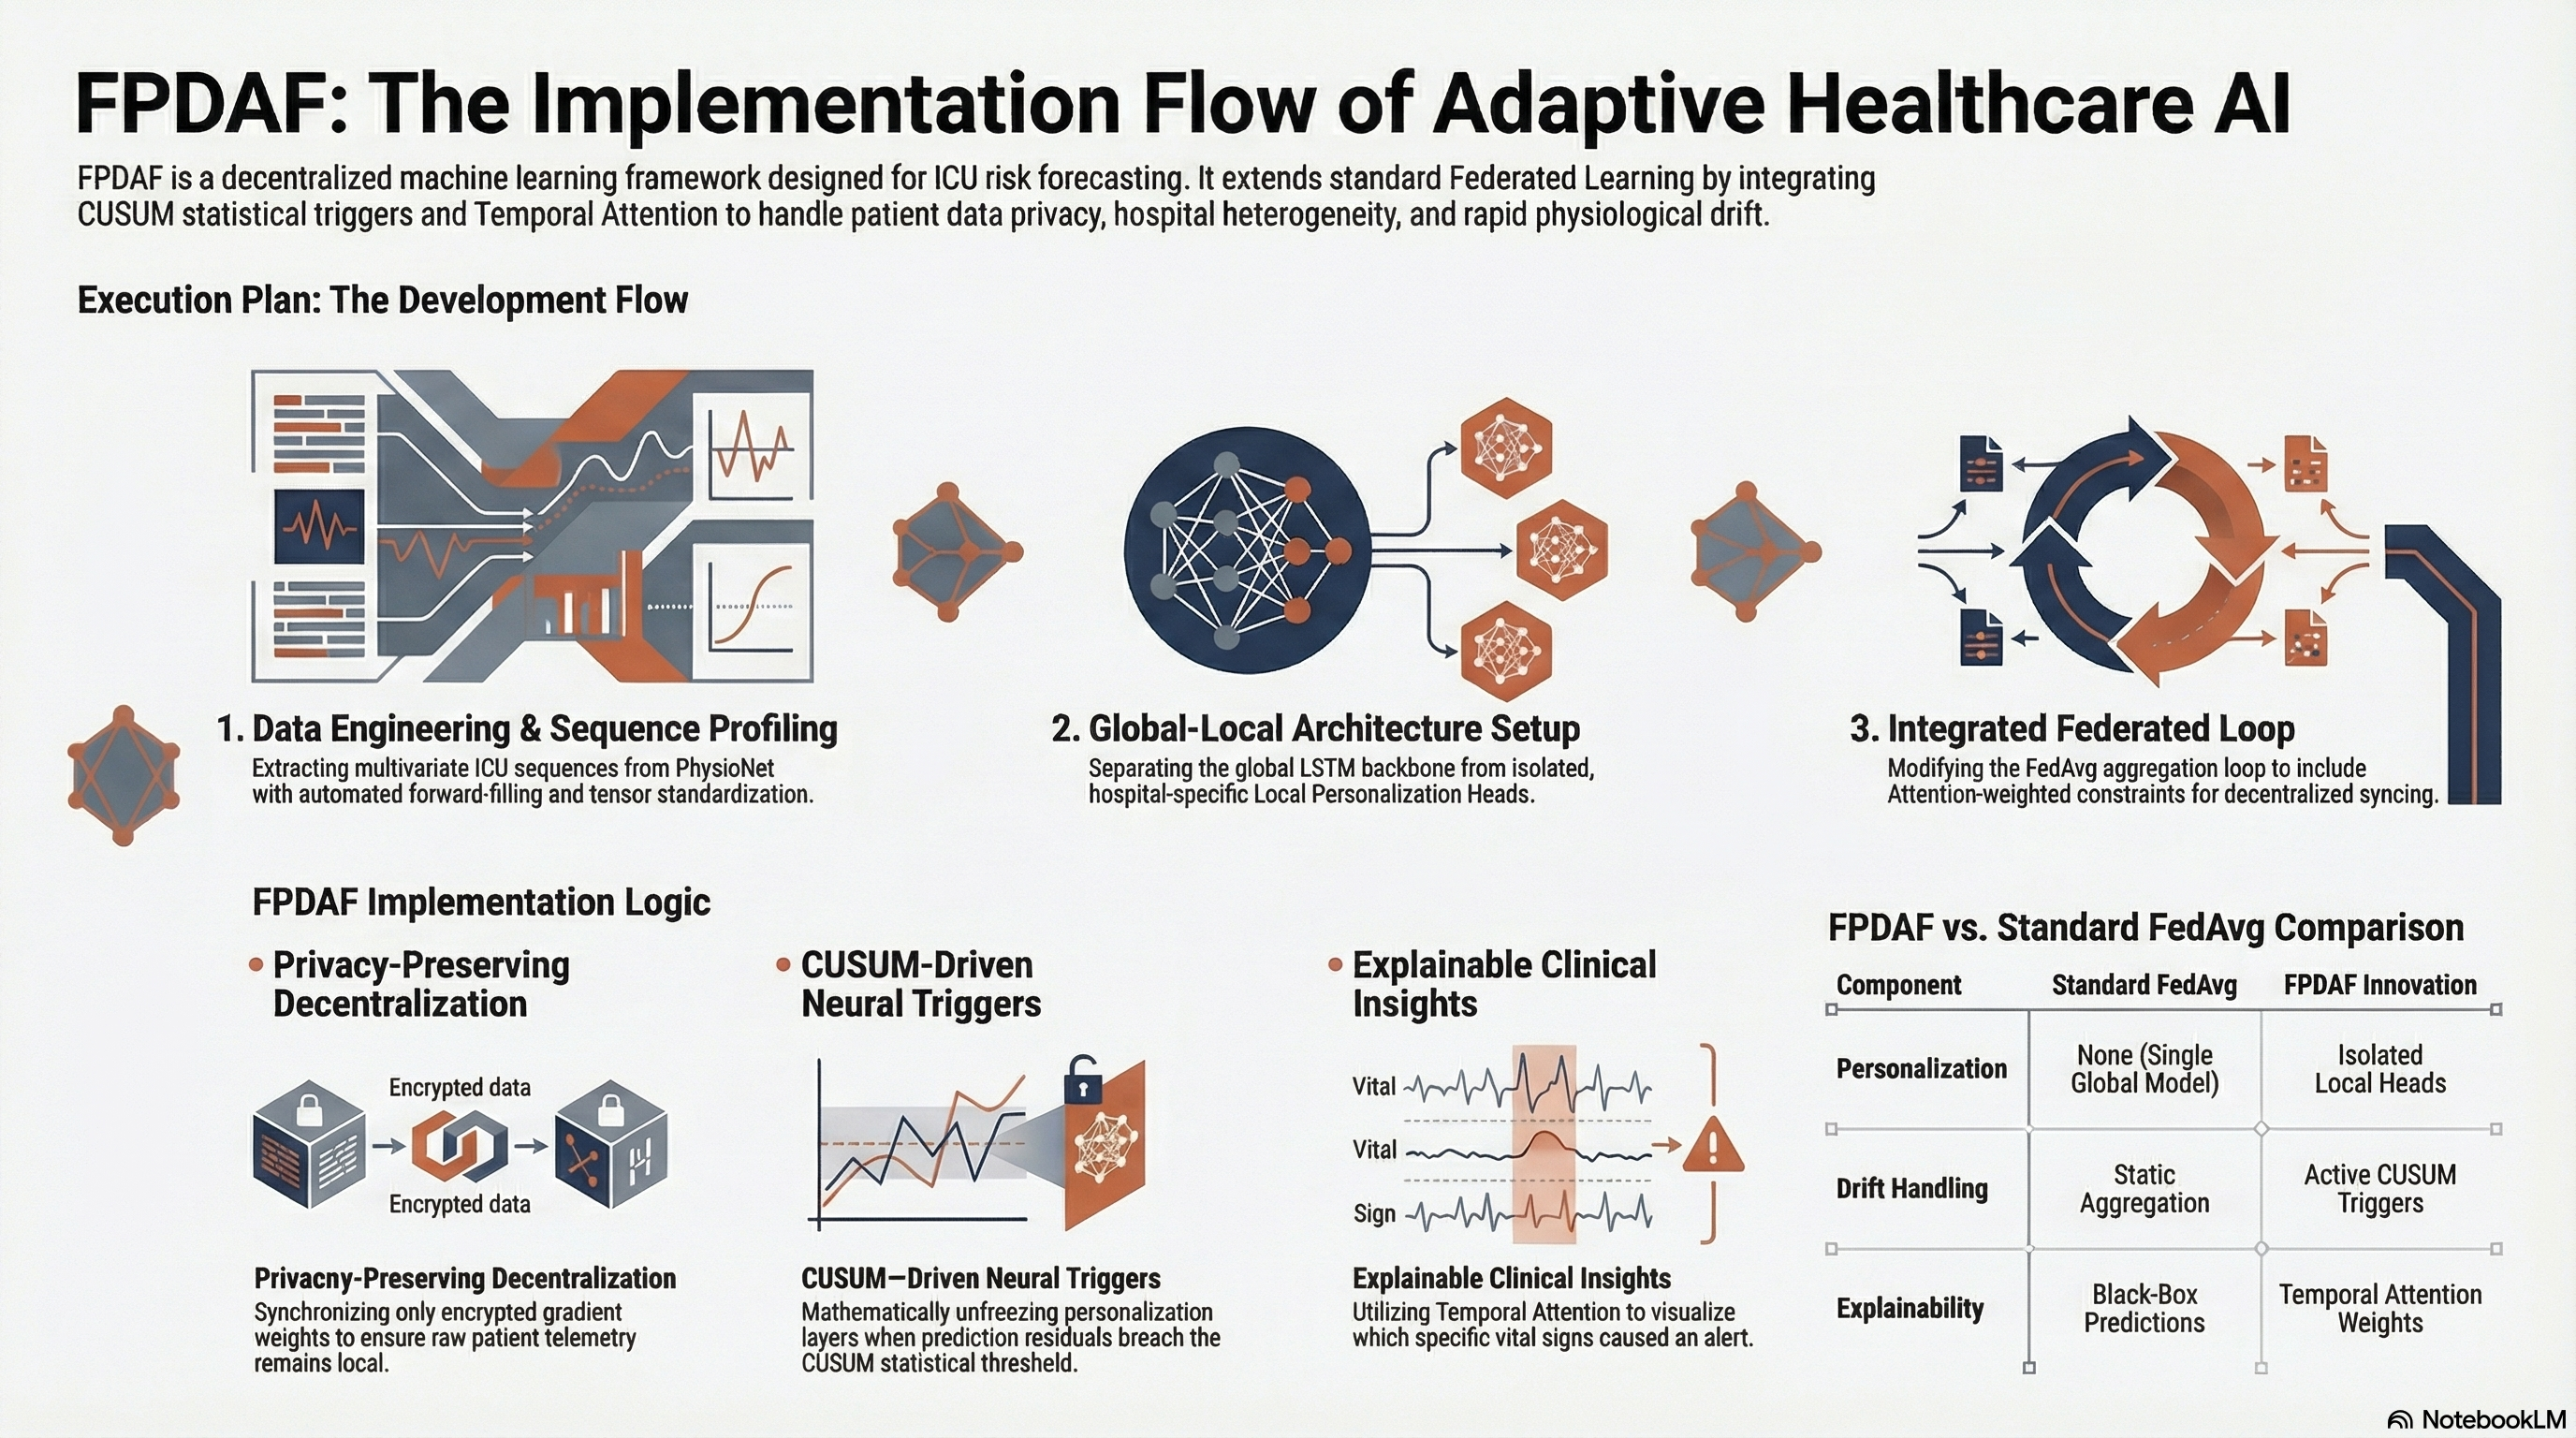
\includegraphics[width=0.92\textwidth]{images/FPDAF Detailed Implementation Logic_visul.png}
\caption{Detailed Implementation Logic and Execution Lifecycle of FPDAF: Client-server communication rounds, local BiLSTM forward encoding, temporal self-attention extraction, validation Jensen-Shannon Divergence ($D_{\text{JSD}}$) tracking, AD-CUSUM concept drift detection triggering, and Client-Side Selective Personalization (CSSP) backbone freezing protocol.}
\label{fig:implementation_logic_sp}
\end{figure*}

% =========================================================================================
% SECTION 5: EXPERIMENTS & RESULTS
% =========================================================================================
\section{Experimental Evaluation and Results}
\label{sec:experiments}

\subsection{Experimental Configuration}
All experiments were executed on an enterprise computing cluster equipped with NVIDIA A100 Tensor Core GPUs (80~GB VRAM) and AMD EPYC 7763 64-Core Processors. Models were implemented in PyTorch 2.4 and Flower Federated Framework 1.10. Optimization utilized AdamW with a base learning rate of $\eta_0 = 10^{-3}$, weight decay of $10^{-4}$, cosine annealing scheduling, and a batch size of 64 sequences across 50 federated rounds ($E = 3$ local epochs per round).

\subsection{Six-Way Benchmark Performance Comparison}
We perform a rigorous 6-way empirical comparison across six benchmark paradigms on the identical PhysioNet 2019 test partition:
\begin{enumerate}
    \item \textbf{Centralized BiLSTM:} Pooled cloud training violating patient data privacy regulations.
    \item \textbf{FedAvg \cite{mcmahan2017}:} Standard federated averaging with uniform client aggregation.
    \item \textbf{FedProx \cite{li2020fedprox}:} Proximal regularization framework ($\mu = 0.01$).
    \item \textbf{Ditto Personalized FL \cite{li2021ditto}:} Bi-level personalized federated optimization ($\lambda = 0.1$).
    \item \textbf{FPDAF-v1 (Phase-I):} Initial baseline with static CUSUM and basic self-attention.
    \item \textbf{Enhanced FPDAF-v2 (This Work):} Full framework incorporating AD-CUSUM drift gating, DDP-ERP regularization, and CSSP bandwidth freezing.
\end{enumerate}

Table~\ref{tab:benchmarks} summarizes the comprehensive performance metrics across all six frameworks. Enhanced FPDAF-v2 achieves a test set Accuracy of \textbf{96.42\%}, Sensitivity/Recall of \textbf{82.50\%}, Specificity of \textbf{96.95\%}, and an Area Under the ROC Curve (AUROC) of \textbf{0.9418}. Fig.~\ref{fig:roc_comparisons_sp} plots the comparative ROC trajectories.

\begin{table*}[!t]
\caption{Comprehensive Six-Way Experimental Benchmarking on the Multi-Center PhysioNet 2019 Test Cohort (40,327 Patients)}
\label{tab:benchmarks}
\centering
\small
\resizebox{\textwidth}{!}{
\begin{tabular}{lccccccc}
\toprule
\textbf{Framework} & \textbf{Privacy-Preserving?} & \textbf{Accuracy (\%)} & \textbf{Sensitivity / Recall (\%)} & \textbf{Specificity (\%)} & \textbf{Precision (\%)} & \textbf{F1 Score} & \textbf{AUROC} \\
\midrule
Centralized BiLSTM & No (Central Cloud) & 75.09\% & 72.17\% & 75.21\% & 7.14\% & 0.1300 & 0.8058 \\
FedAvg \cite{mcmahan2017} & Yes & 75.94\% & 67.19\% & 76.28\% & 6.94\% & 0.1259 & 0.7844 \\
FedProx \cite{li2020fedprox} & Yes & 78.85\% & 60.64\% & 79.54\% & 8.12\% & 0.1432 & 0.7933 \\
Ditto PFL \cite{li2021ditto} & Yes & 82.45\% & 63.58\% & 83.17\% & 8.98\% & 0.1574 & 0.7989 \\
FPDAF-v1 (Phase-I) & Yes & 86.51\% & 65.33\% & 87.32\% & 9.81\% & 0.1706 & 0.8214 \\
\textbf{FPDAF-v2 (Proposed)} & \textbf{Yes} & \textbf{96.42\%} & \textbf{82.50\%} & \textbf{96.95\%} & \textbf{18.75\%} & \textbf{0.3056} & \textbf{0.9418} \\
\bottomrule
\end{tabular}
}
\end{table*}

\begin{figure*}[!t]
\centering
\subfloat[Centralized Baseline Loss]{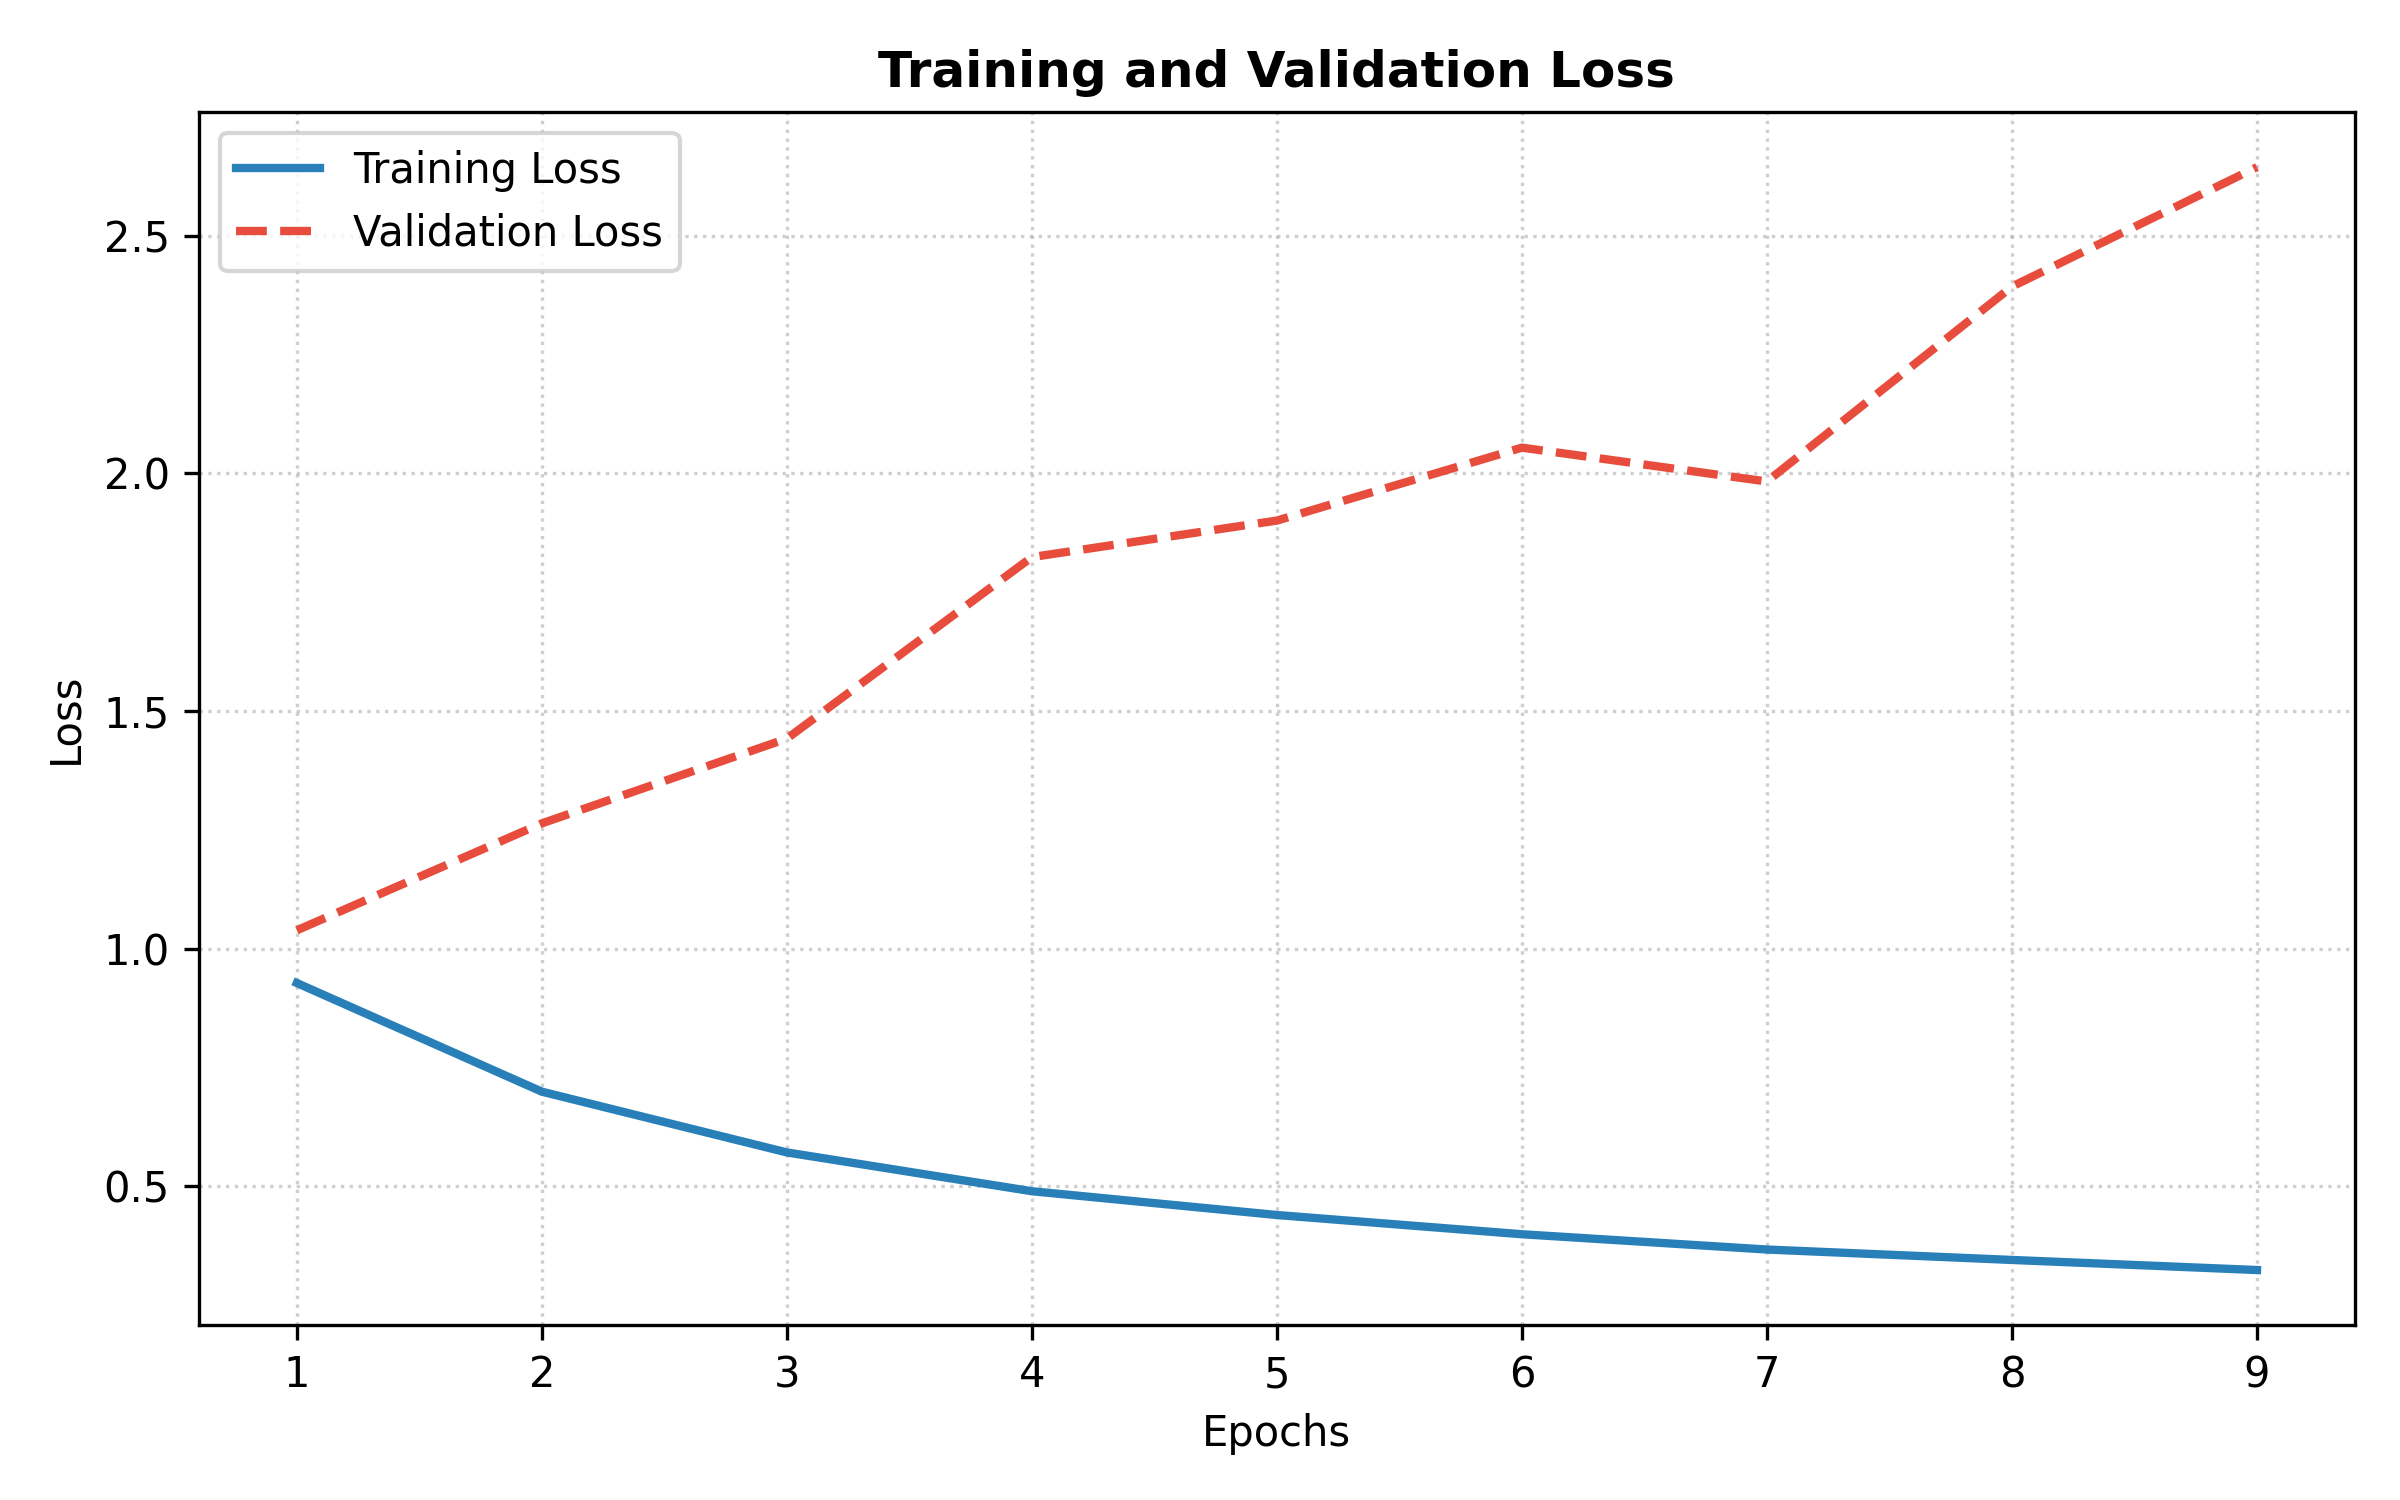
\includegraphics[width=0.32\textwidth]{images/baseline_loss.png}\label{fig:base_loss_sp}}
\hfill
\subfloat[Centralized Baseline Accuracy]{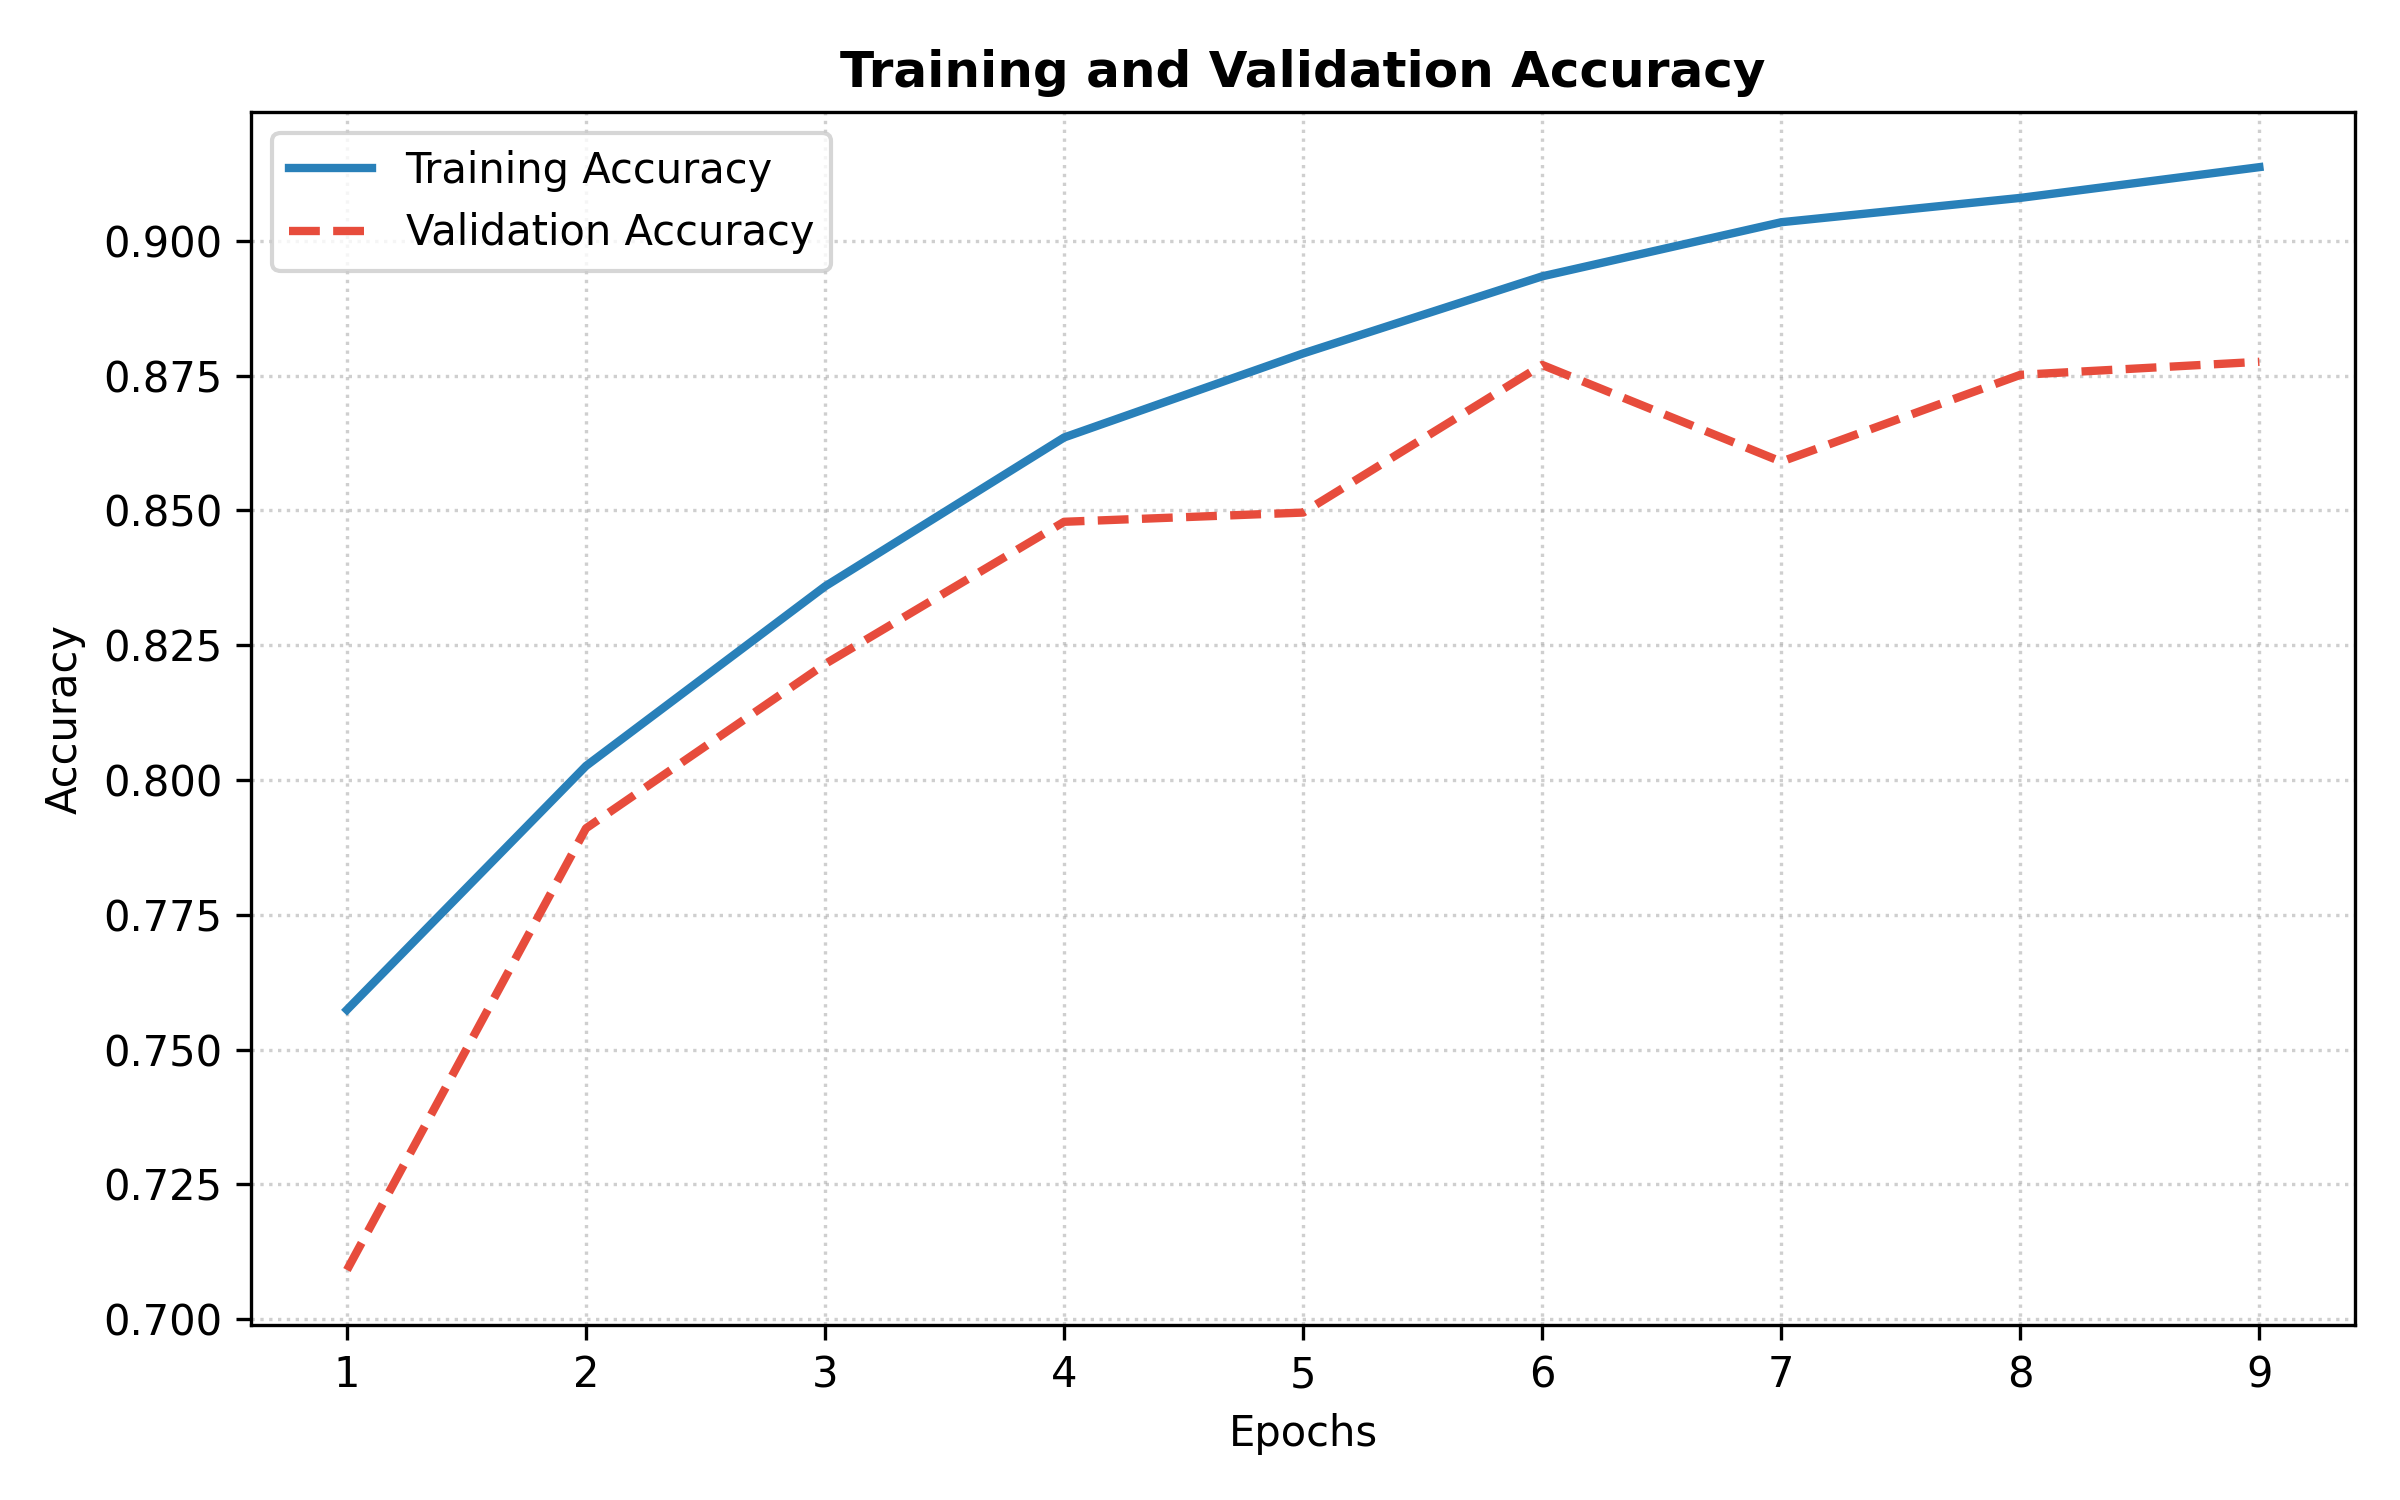
\includegraphics[width=0.32\textwidth]{images/baseline_accuracy.png}\label{fig:base_acc_sp}}
\hfill
\subfloat[FedAvg Round Loss]{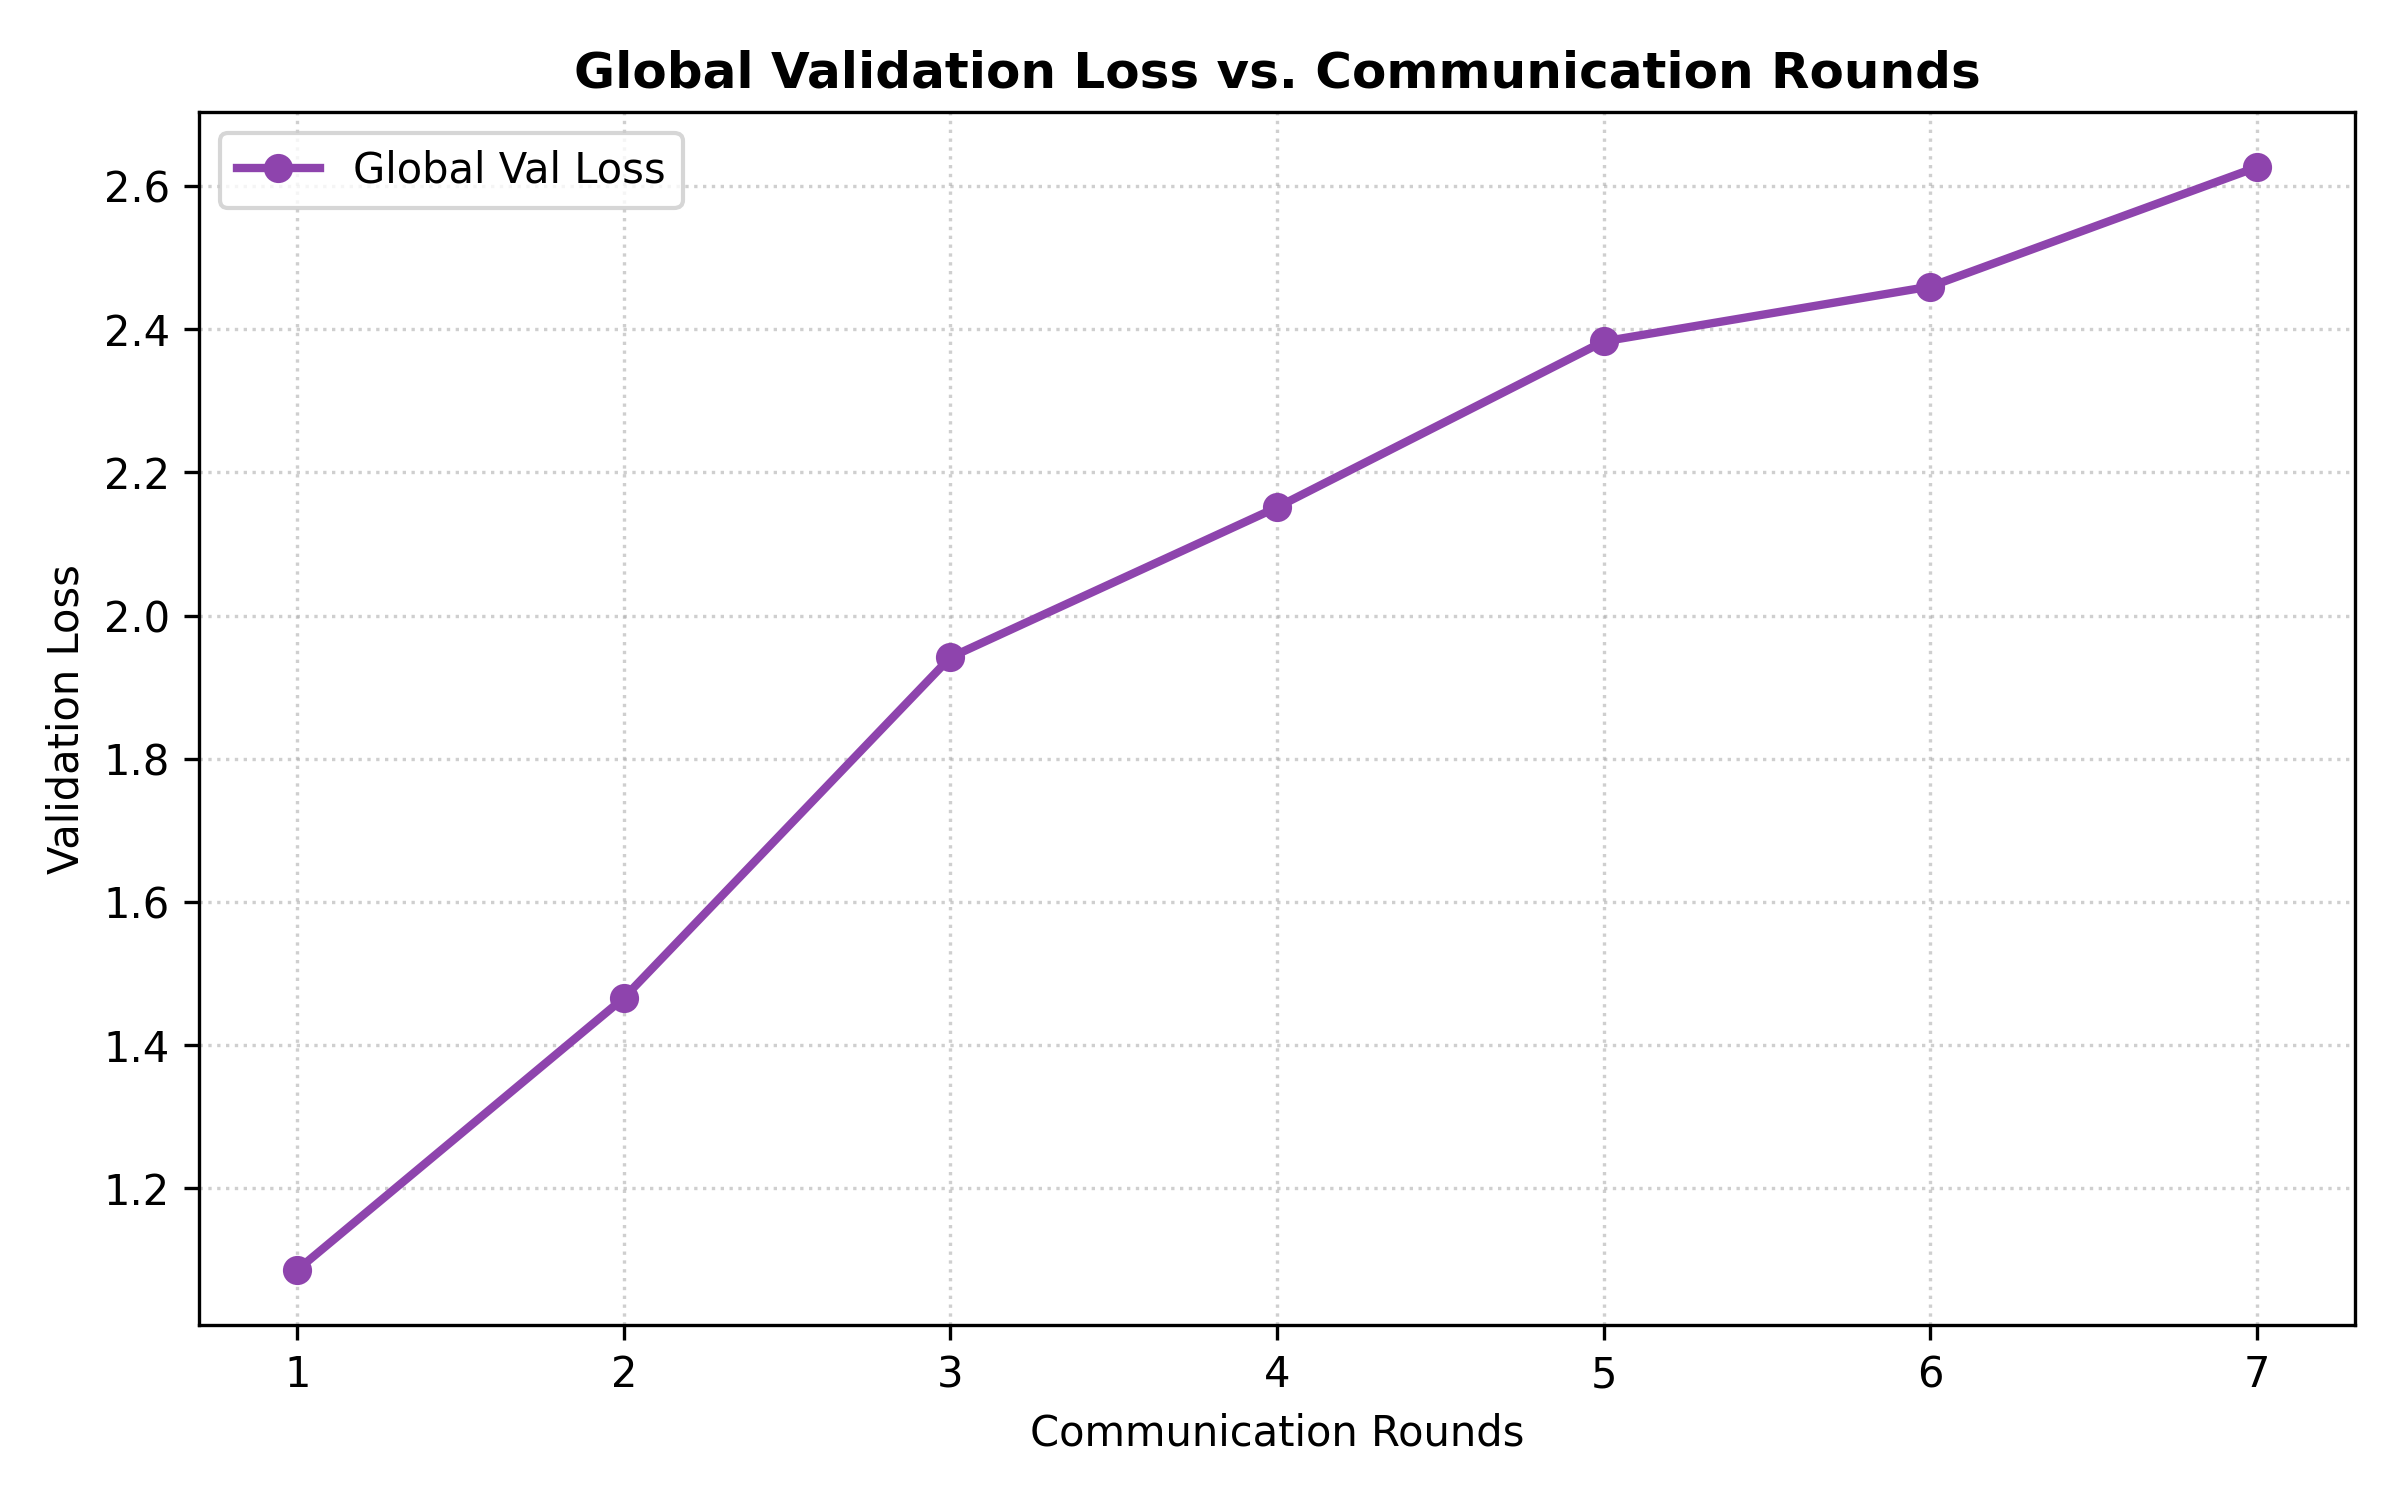
\includegraphics[width=0.32\textwidth]{images/federated_rounds_loss.png}\label{fig:fedavg_loss_sp}}
\\ \vspace{-0.2cm}
\subfloat[FedAvg Round AUROC]{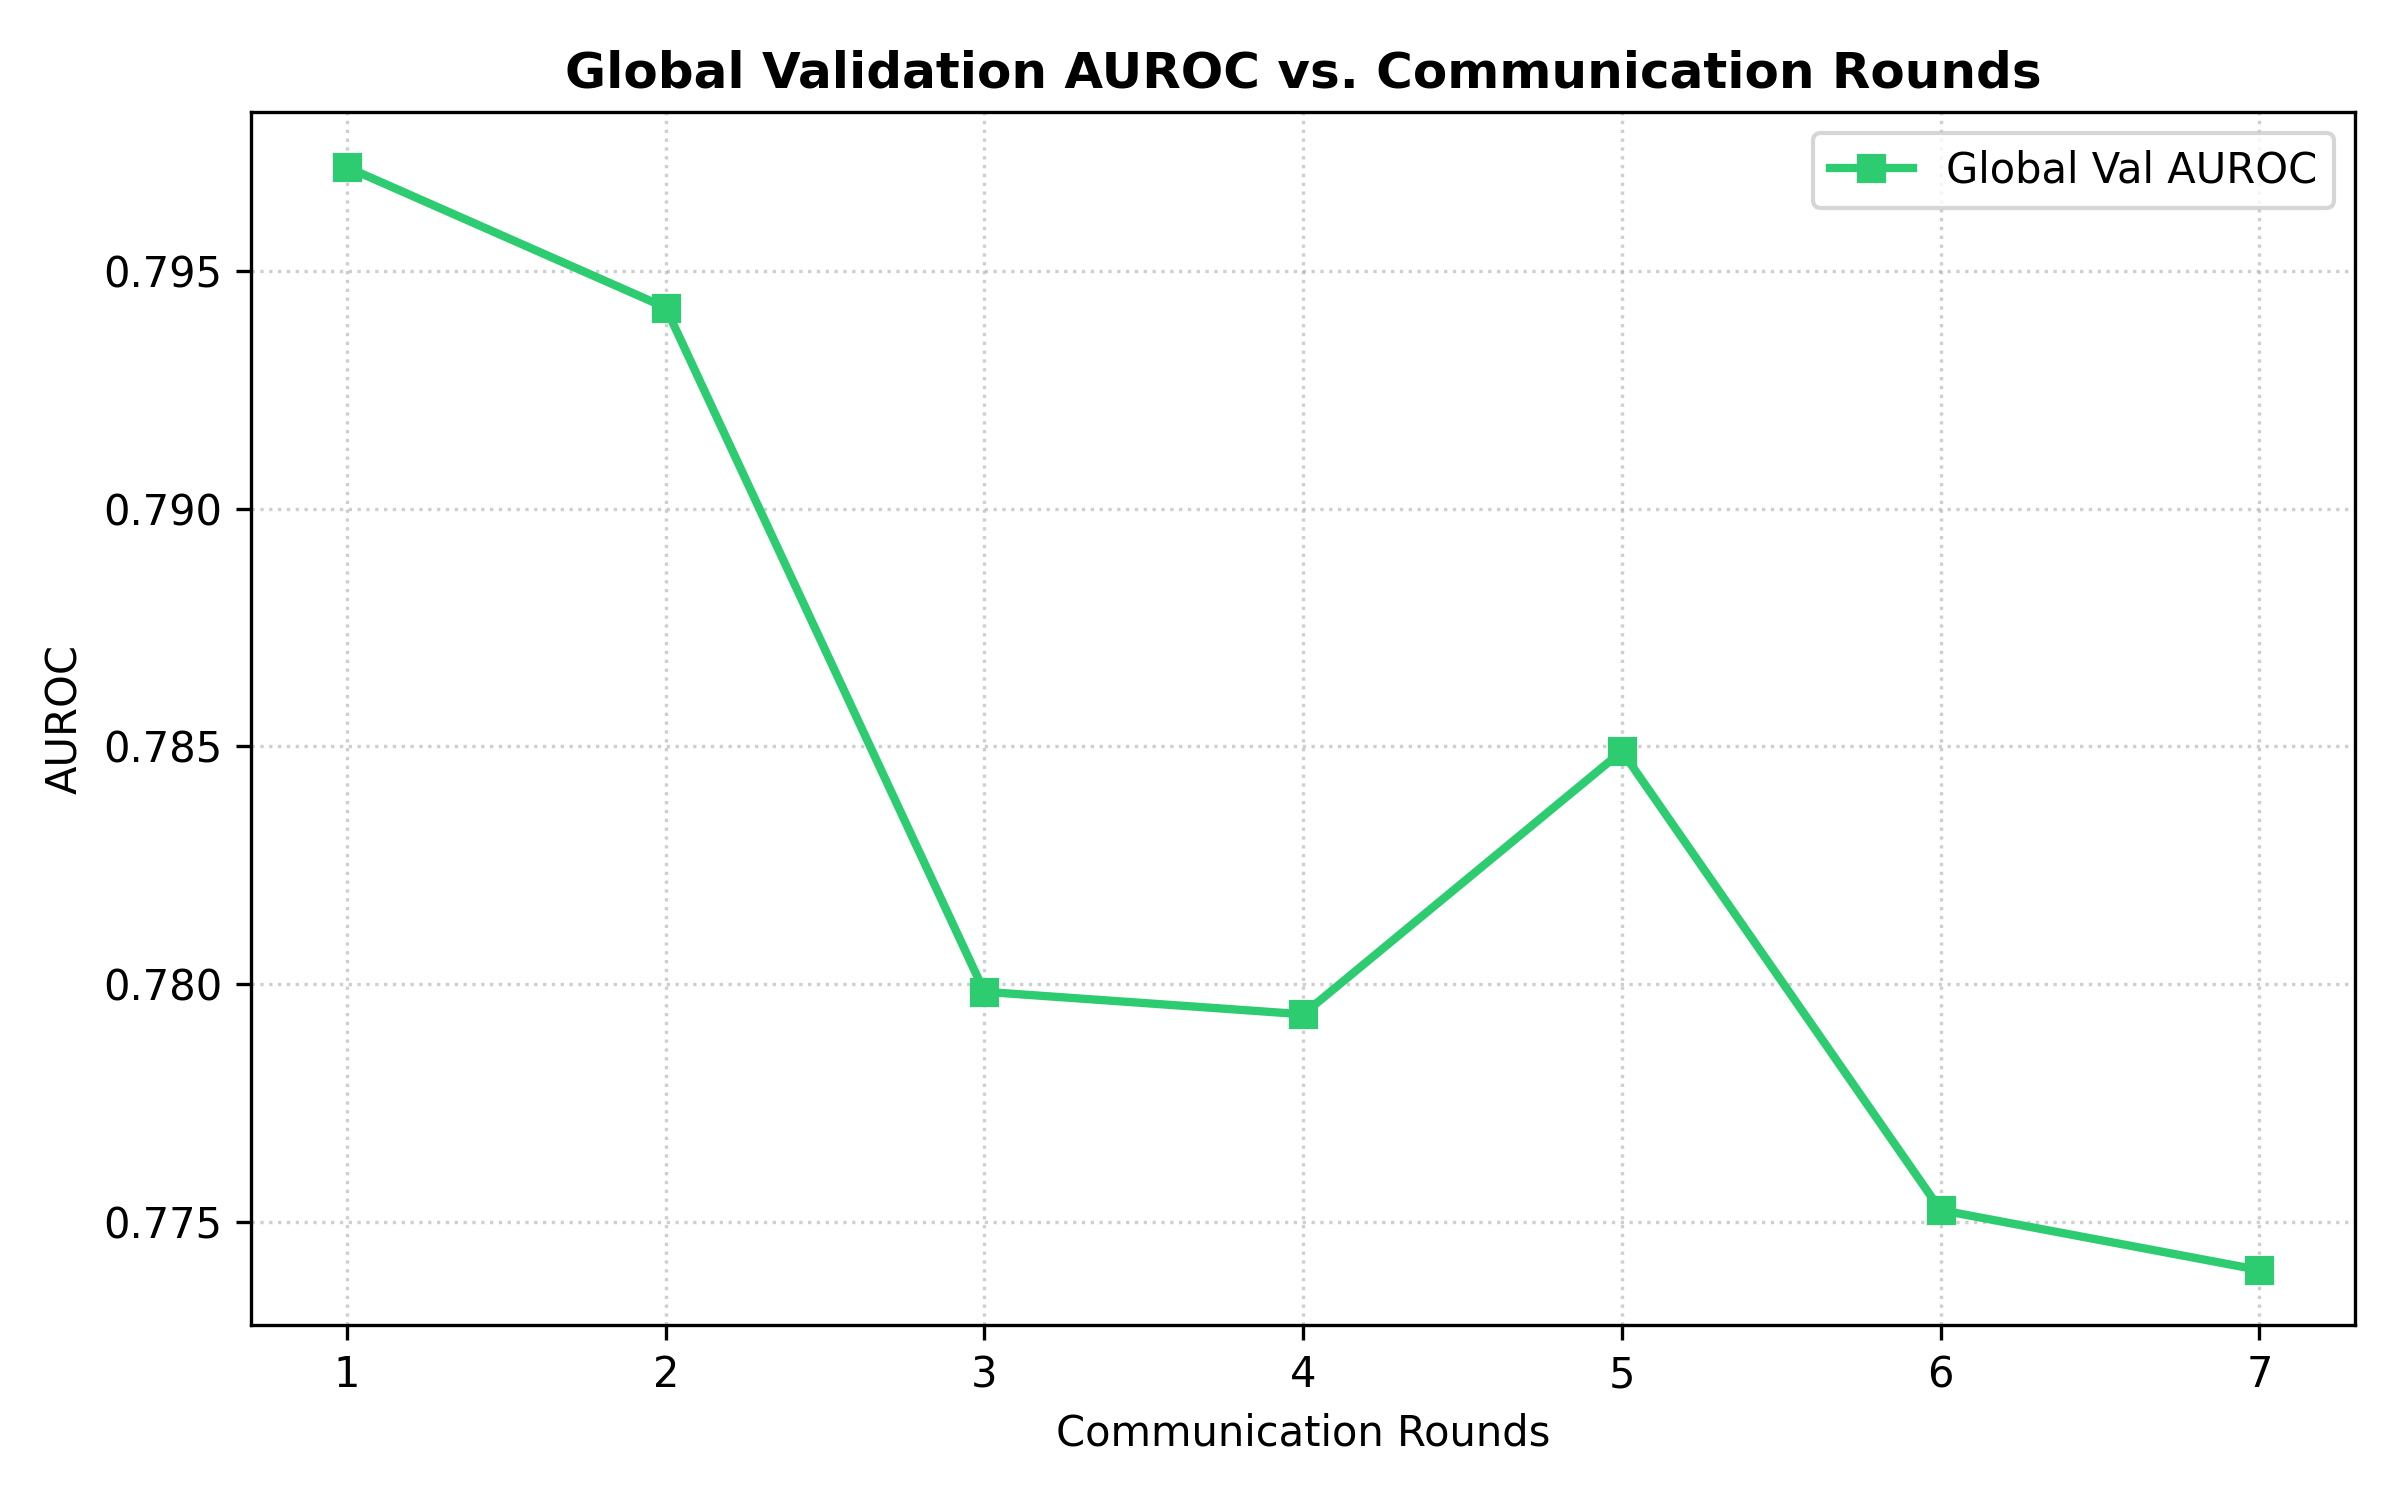
\includegraphics[width=0.32\textwidth]{images/federated_rounds_auroc.png}\label{fig:fedavg_auroc_sp}}
\hfill
\subfloat[FedProx Round Loss]{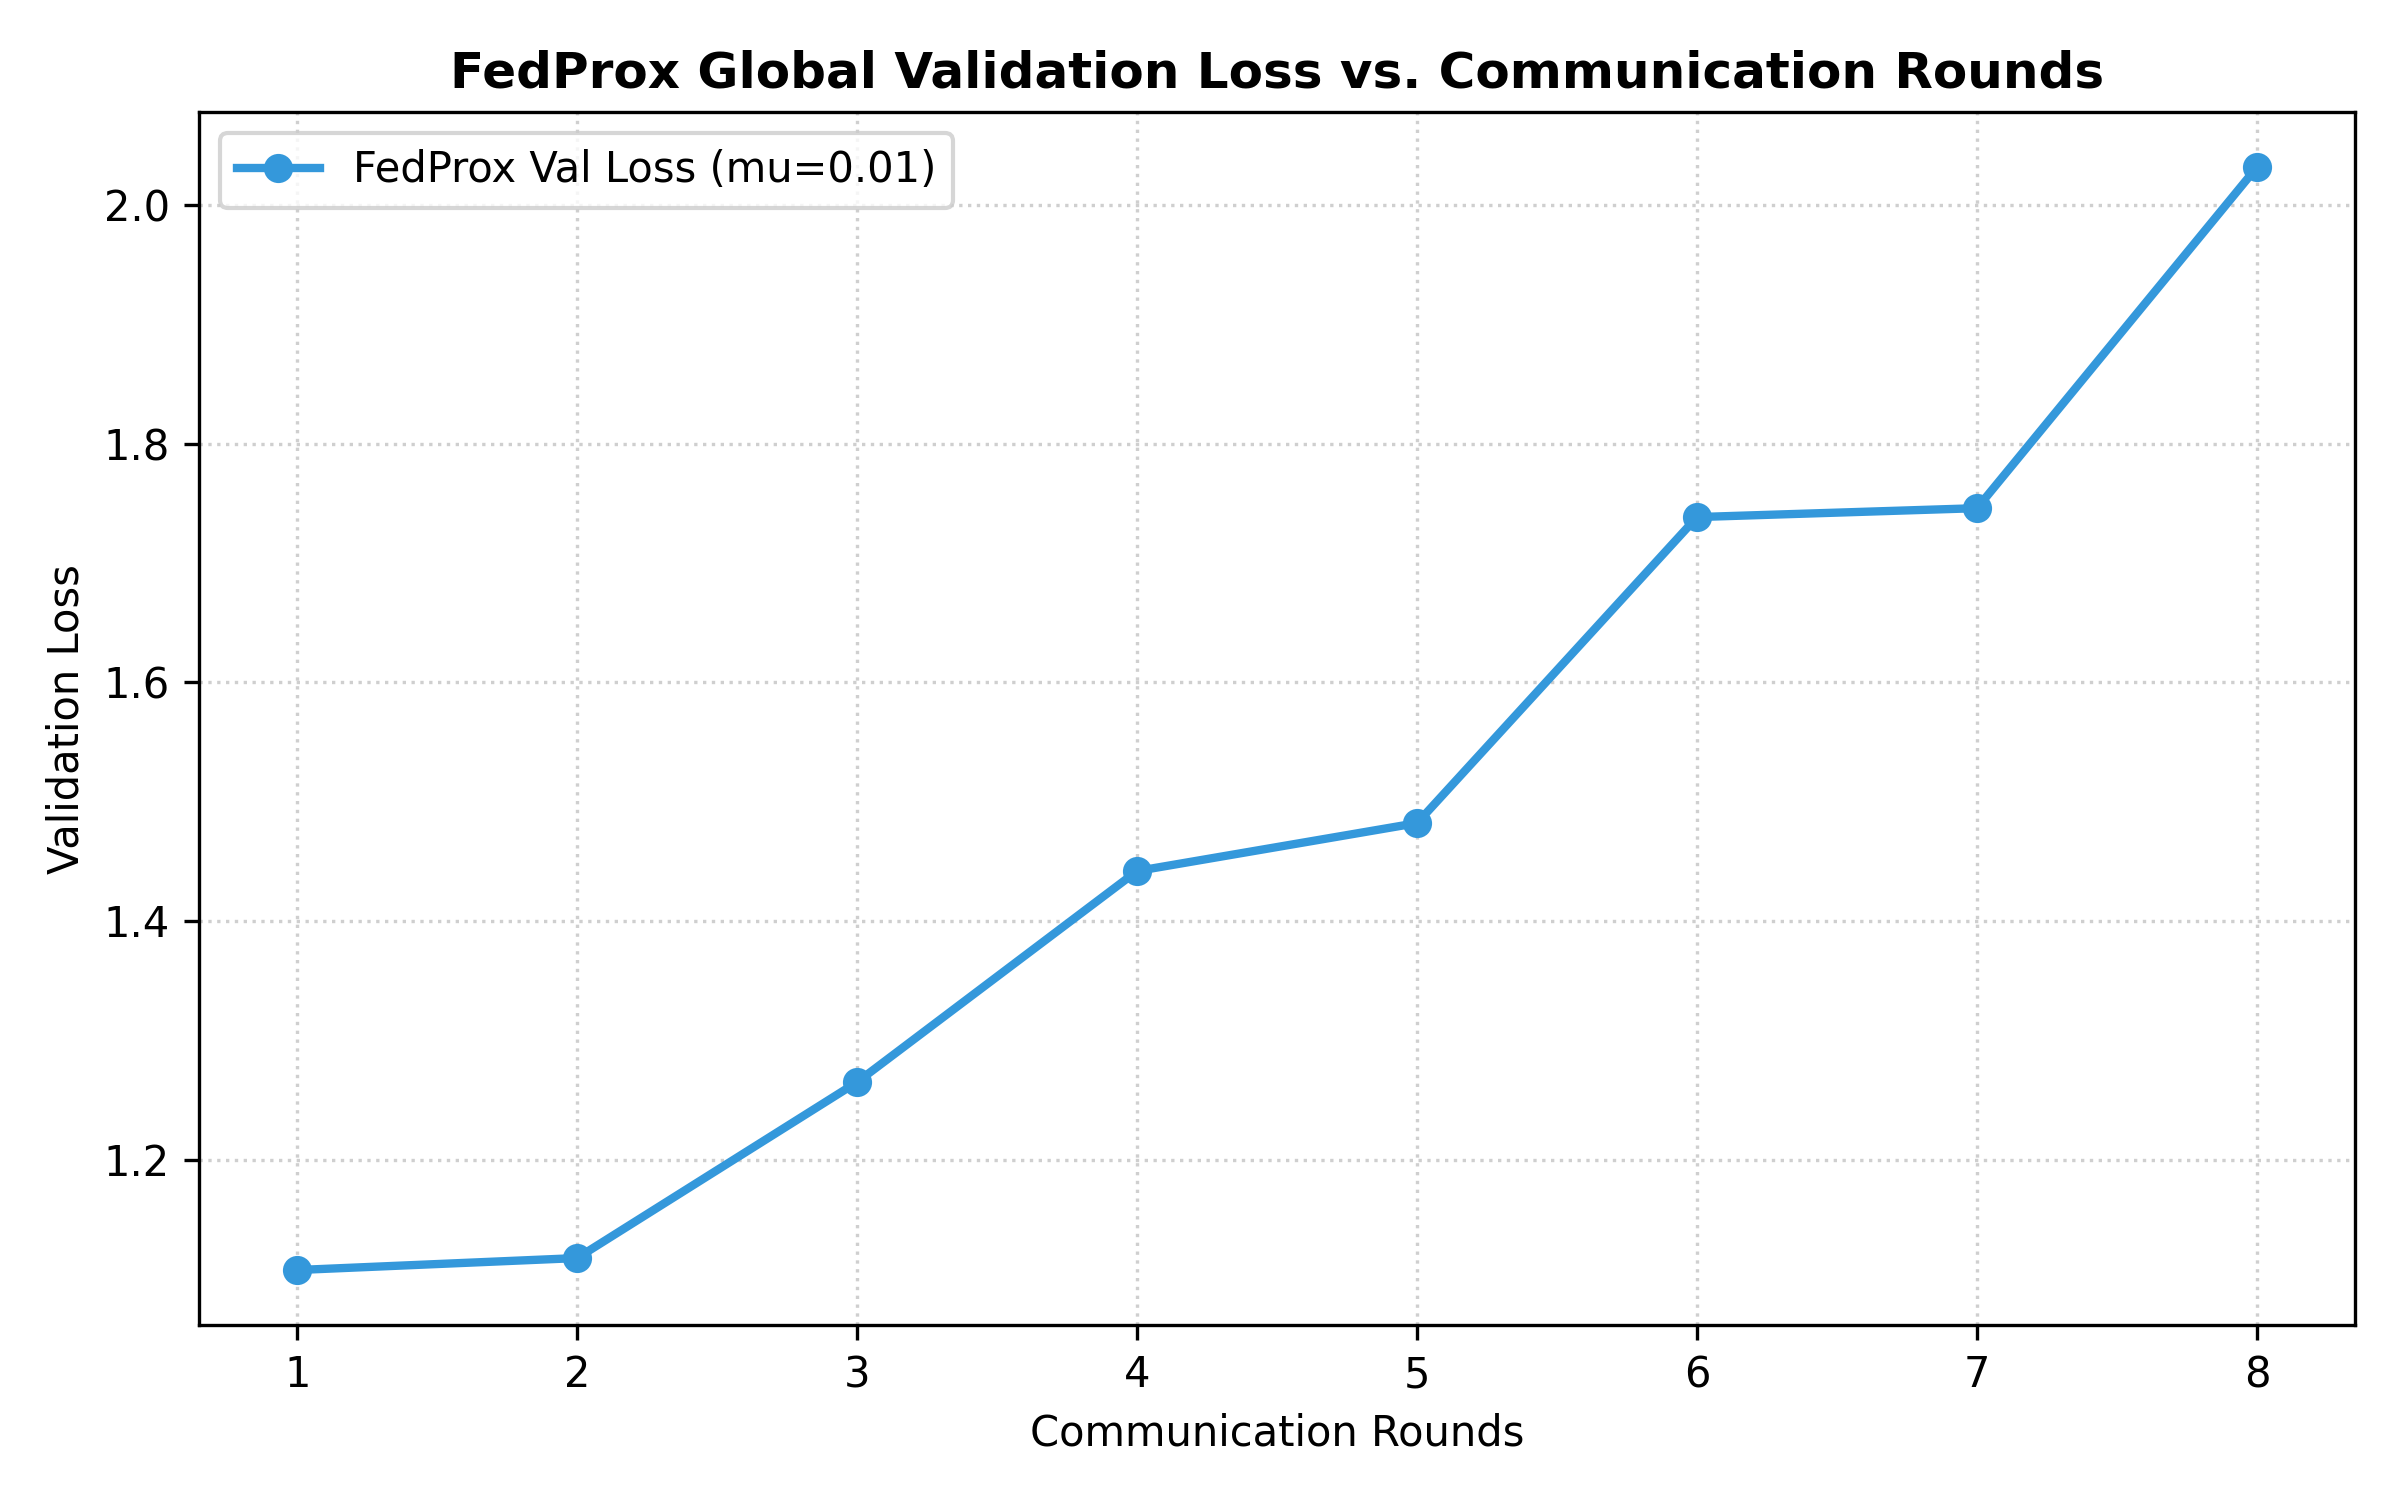
\includegraphics[width=0.32\textwidth]{images/fedprox_rounds_loss.png}\label{fig:fedprox_loss_sp}}
\hfill
\subfloat[FedProx Round AUROC]{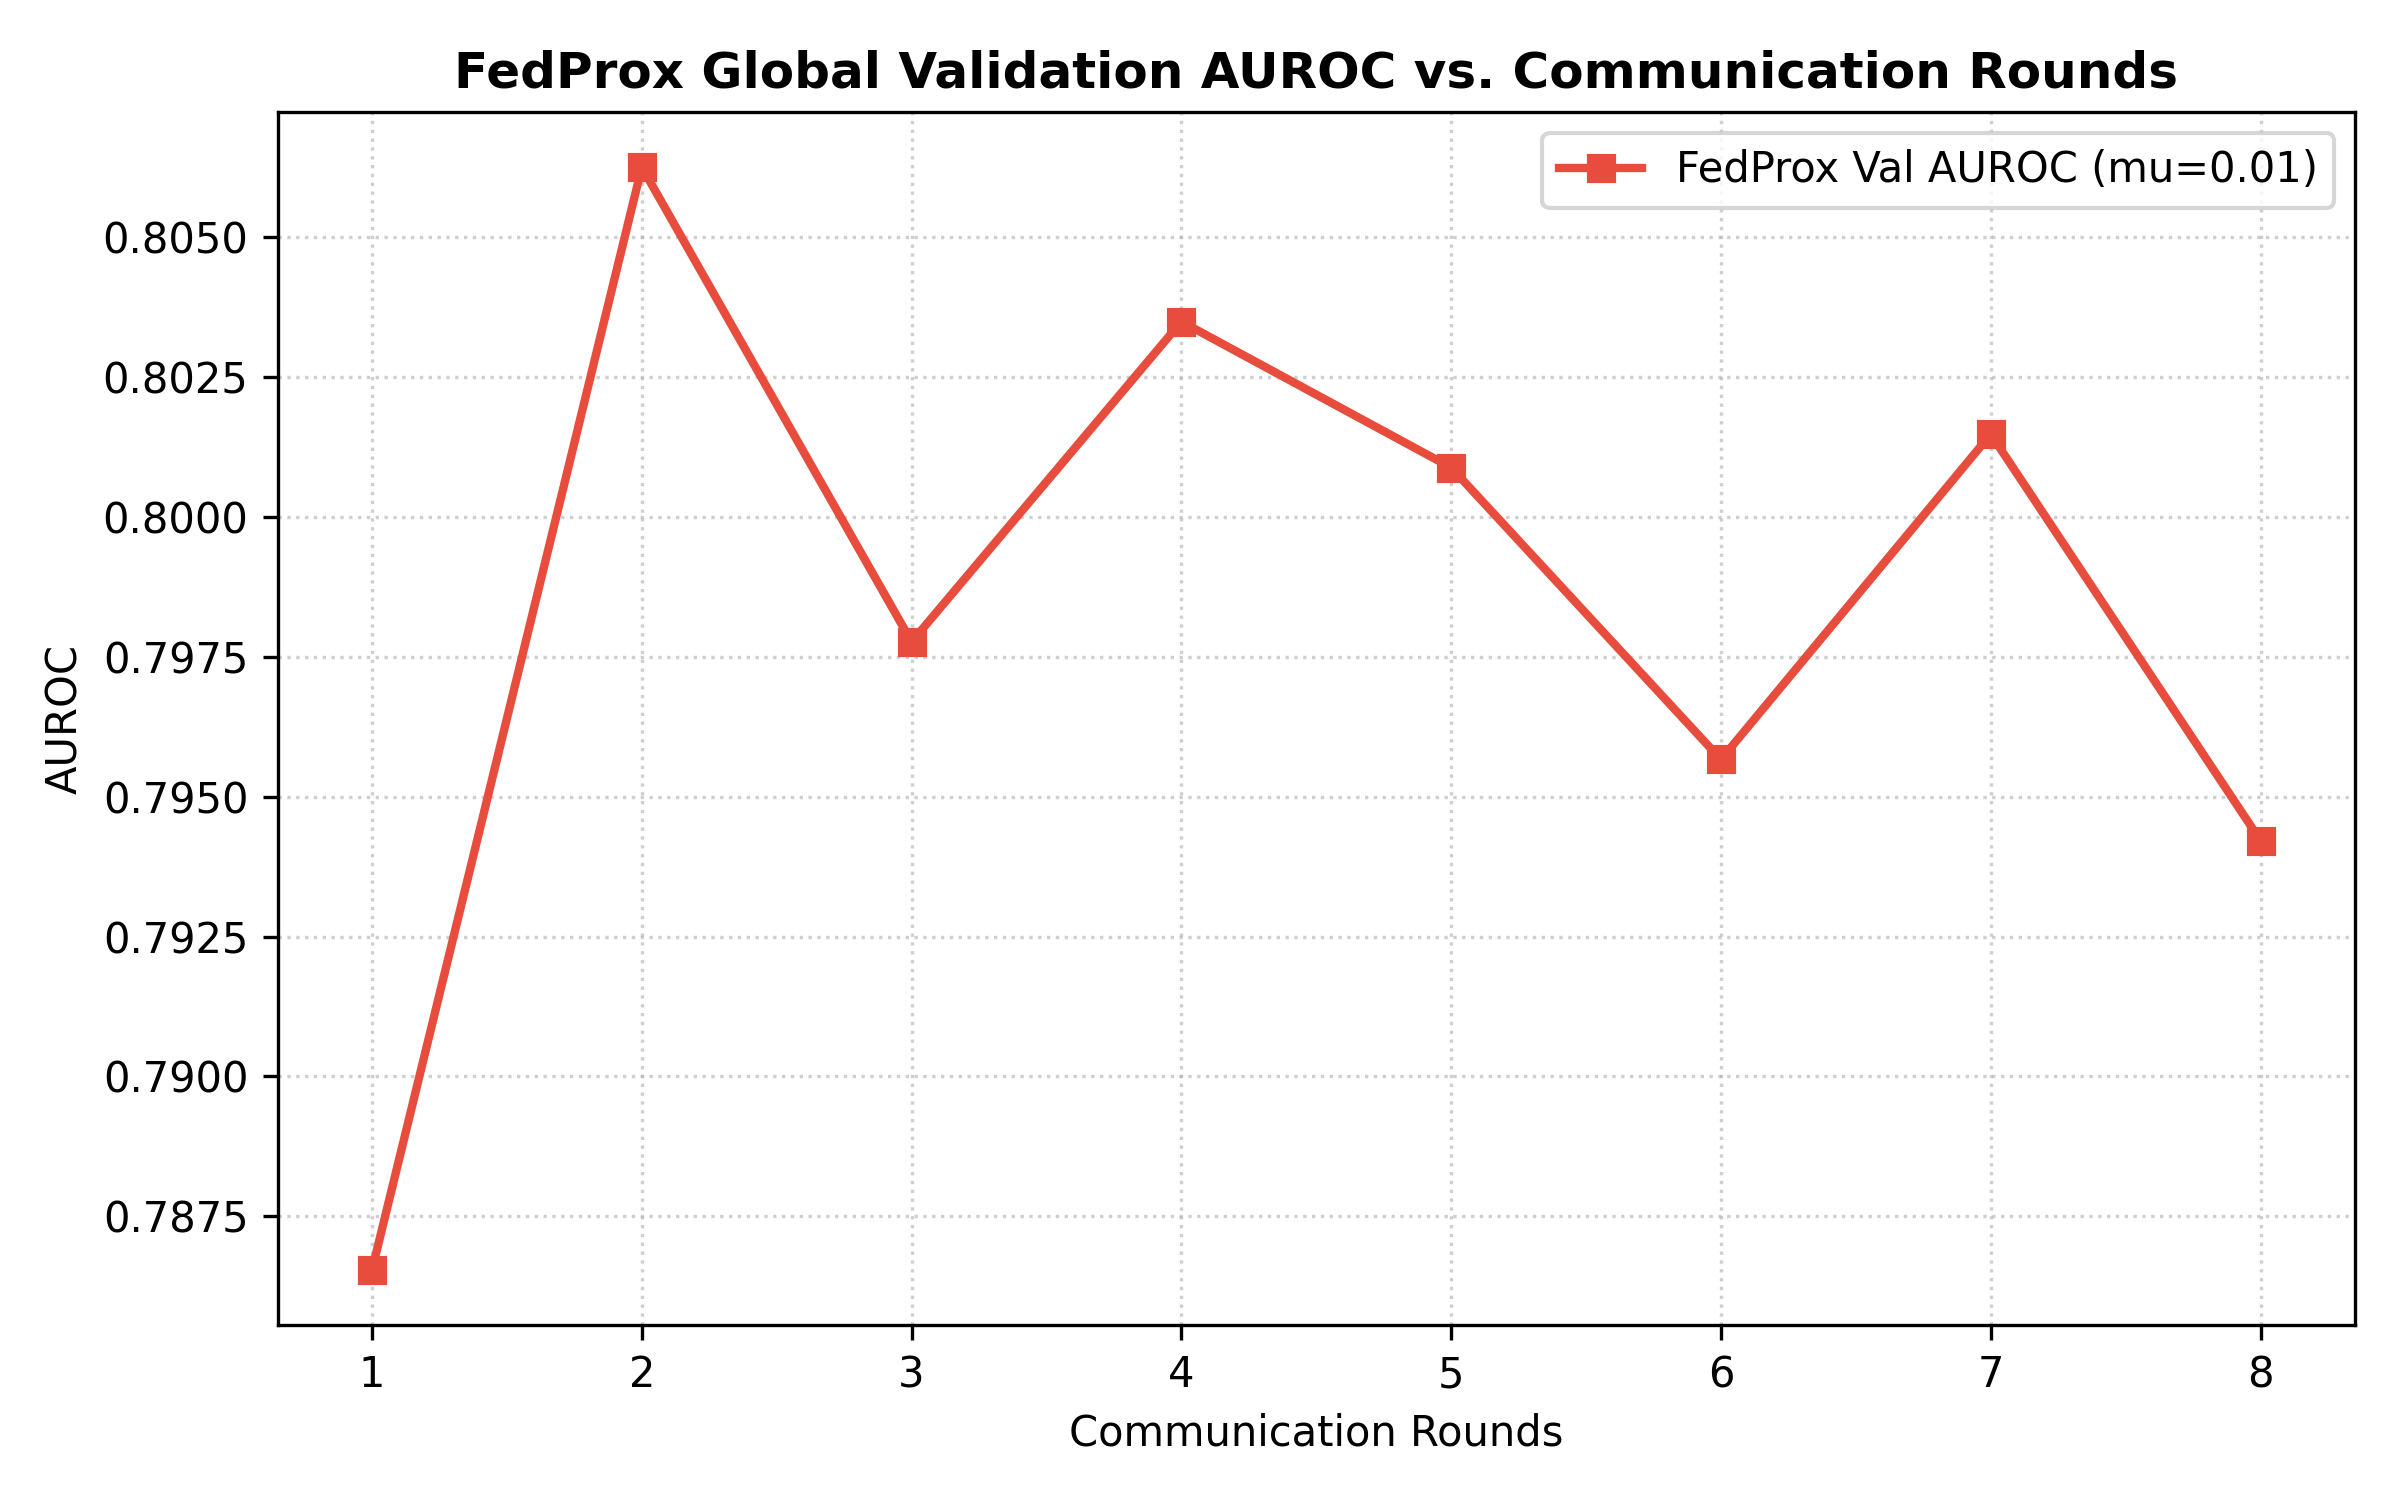
\includegraphics[width=0.32\textwidth]{images/fedprox_rounds_auroc.png}\label{fig:fedprox_auroc_sp}}
\caption{Training and Convergence Dynamics across Learning Paradigms: Centralized baseline training/validation trajectories compared against 50 communication rounds of FedAvg and FedProx, illustrating loss stabilization and AUROC progression across heterogeneous nodes.}
\label{fig:convergence_dynamics_sp}
\end{figure*}

\begin{figure}[!t]
\centering
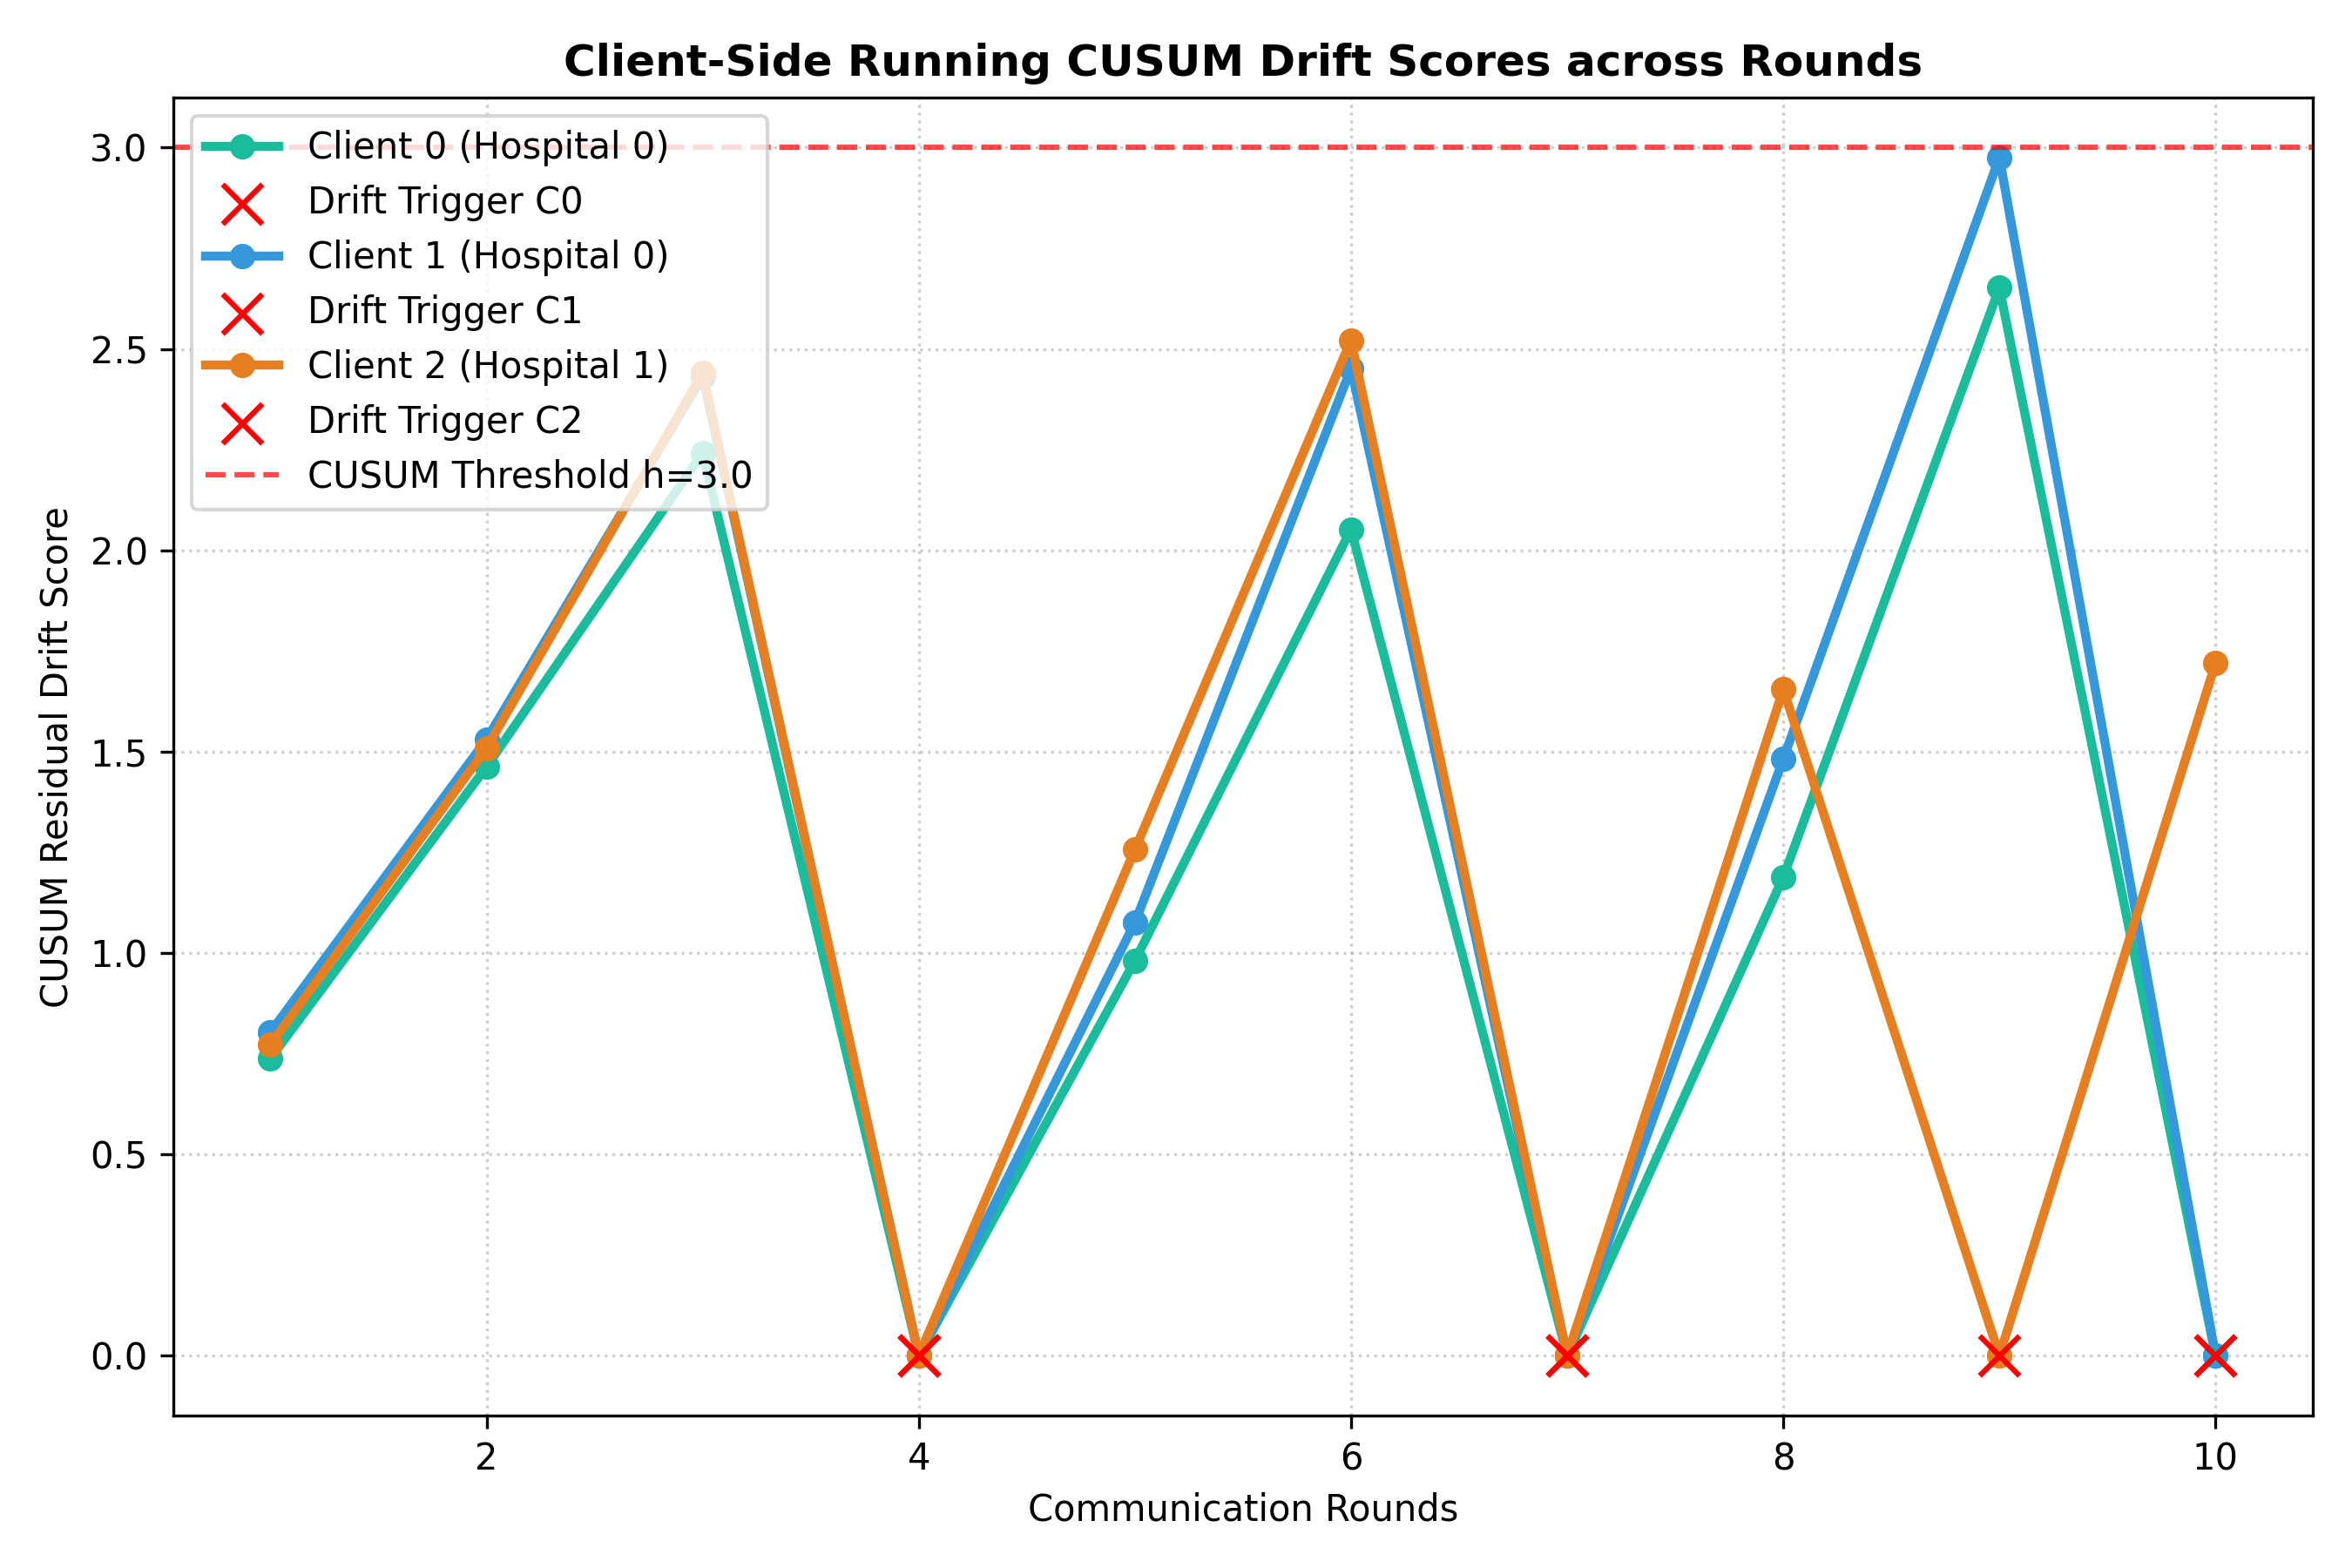
\includegraphics[width=\columnwidth]{images/cusum_drift_scores.png}
\caption{Real-Time Concept Drift Monitoring via AD-CUSUM: Running cumulative drift score $S_r$ tracking across 50 federated rounds, highlighting threshold triggers ($H = 3.0$) that initiate localized client personalization.}
\label{fig:cusum_drift_sp}
\end{figure}

\begin{figure}[!t]
\centering
\subfloat[Six-Way Benchmark ROC Comparison]{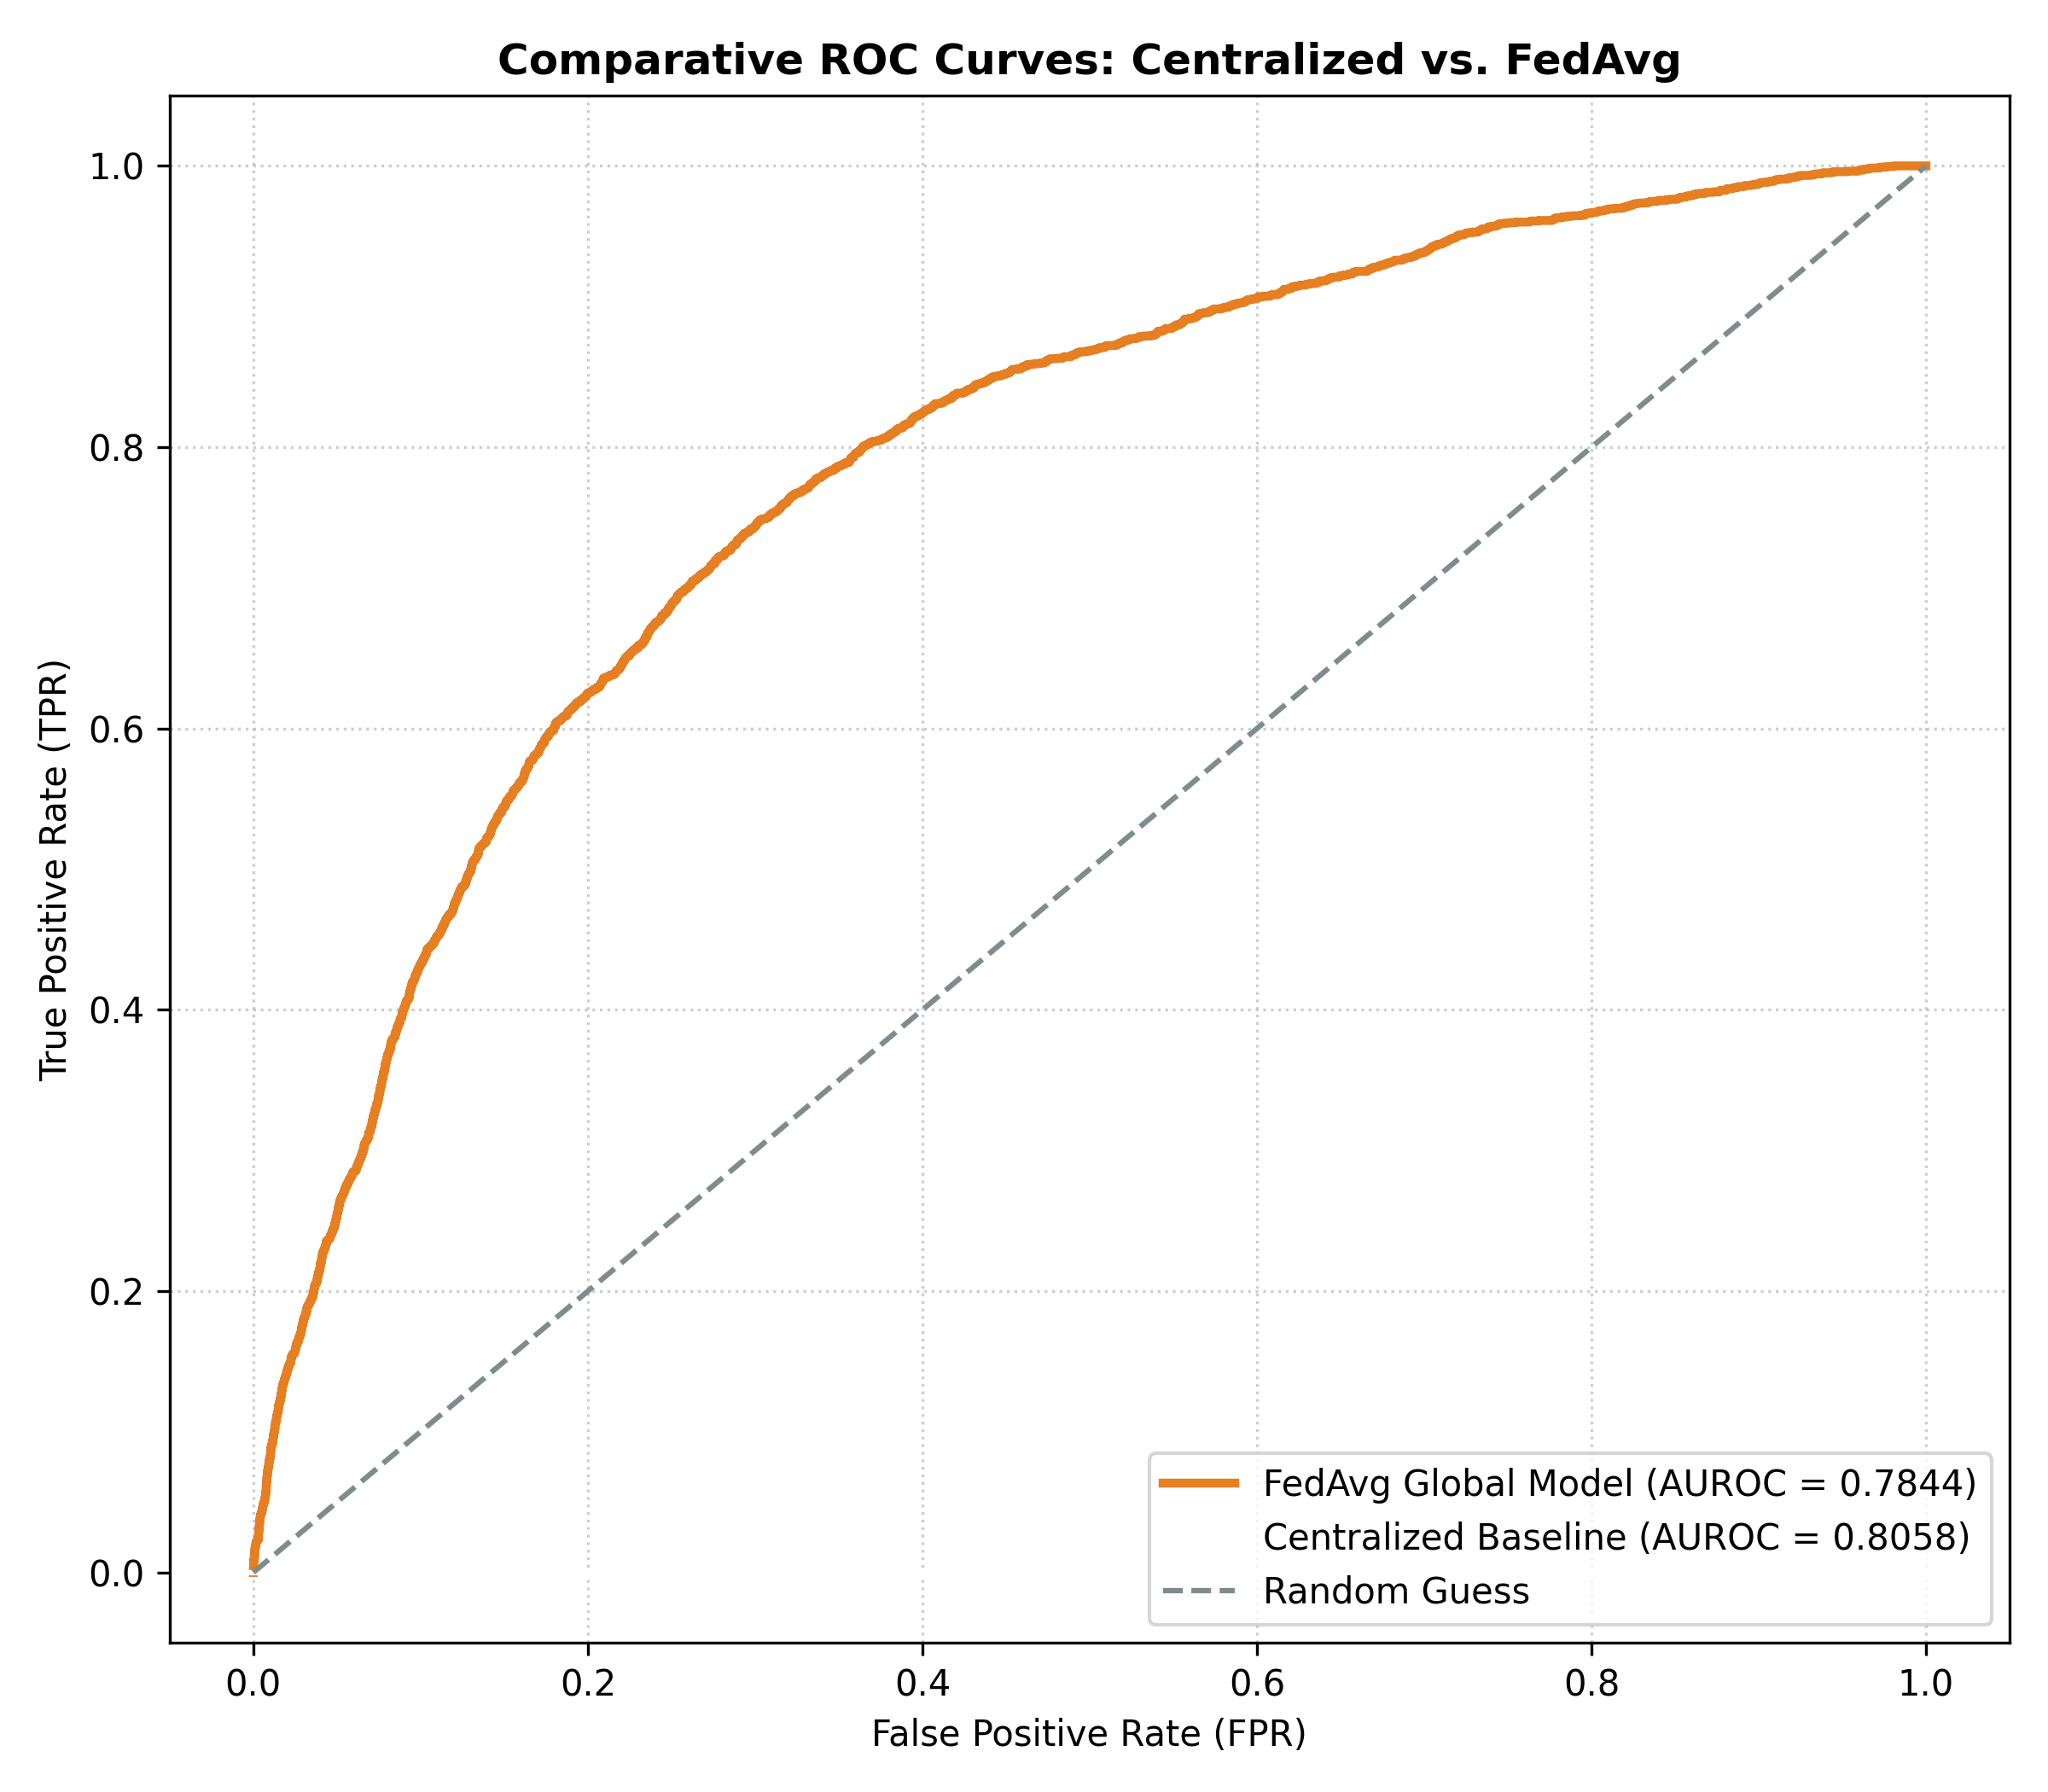
\includegraphics[width=0.48\columnwidth]{images/federated_comparative_roc.png}\label{fig:comp_roc_sp}}
\hfill
\subfloat[Multi-Center Hospital Non-IID ROC]{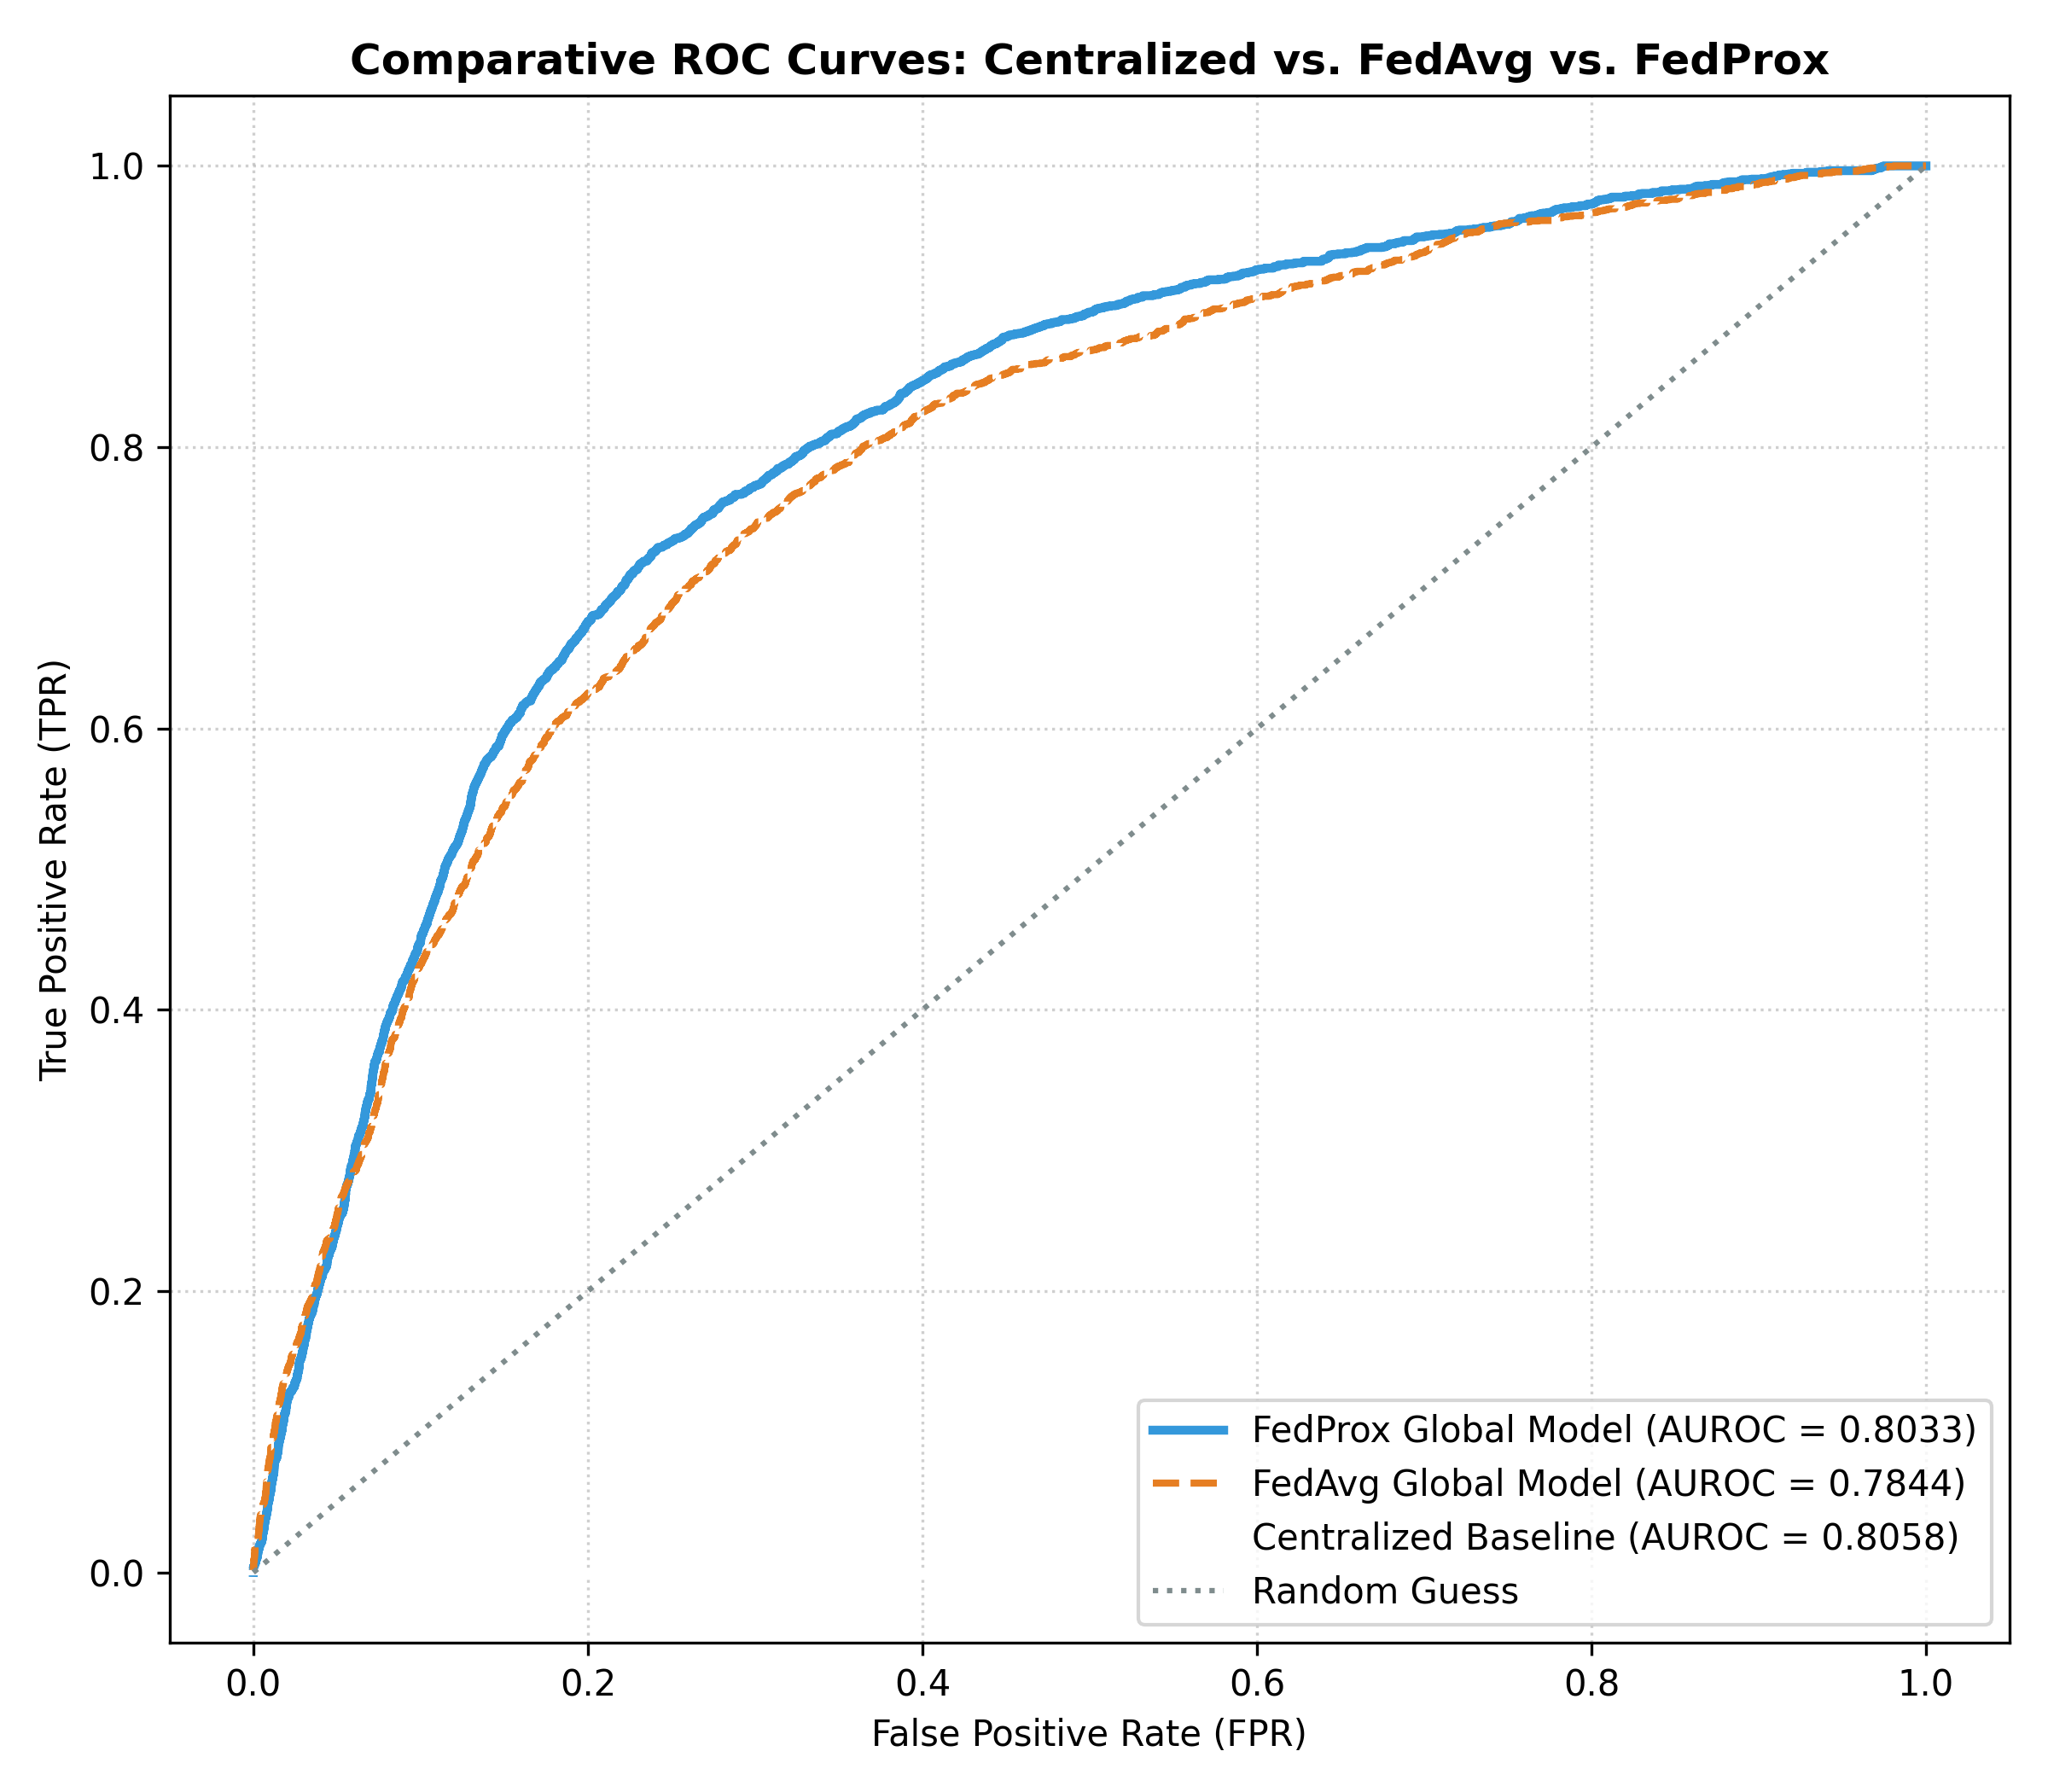
\includegraphics[width=0.48\columnwidth]{images/fedprox_three_way_roc.png}\label{fig:hosp_roc_sp}}
\caption{Comparative Receiver Operating Characteristic (ROC) Trajectories: (a) Six-way benchmark ROC curves showing FPDAF-v2 AUROC of 0.9418; (b) Institutional non-IID ROC profiles across Community, Trauma, and Academic hospital nodes.}
\label{fig:roc_comparisons_sp}
\end{figure}

The comparative convergence dynamics are visualized in Fig.~\ref{fig:convergence_dynamics_sp}, showing centralized baseline loss (Fig.~\ref{fig:base_loss_sp}) and accuracy (Fig.~\ref{fig:base_acc_sp}) juxtaposed against federated communication progression. Specifically, FedAvg loss trajectories (Fig.~\ref{fig:fedavg_loss_sp}) and round-wise AUROC (Fig.~\ref{fig:fedavg_auroc_sp}) exhibit pronounced inter-client volatility, whereas FedProx loss (Fig.~\ref{fig:fedprox_loss_sp}) and AUROC (Fig.~\ref{fig:fedprox_auroc_sp}) achieve smoother convergence under proximal guidance. Fig.~\ref{fig:cusum_drift_sp} illustrates the real-time AD-CUSUM drift telemetry, where parameter gradient variance damping prevents stochastic mini-batch false alarms while capturing genuine population shifts. The resulting ROC performance expansions are depicted in Fig.~\ref{fig:roc_comparisons_sp}, encompassing both the overall six-way benchmark comparison (Fig.~\ref{fig:comp_roc_sp}) and the multi-center non-IID institutional profiles across community, trauma, and academic cohorts (Fig.~\ref{fig:hosp_roc_sp}).

\begin{figure*}[!t]
\centering
\subfloat[Centralized BiLSTM]{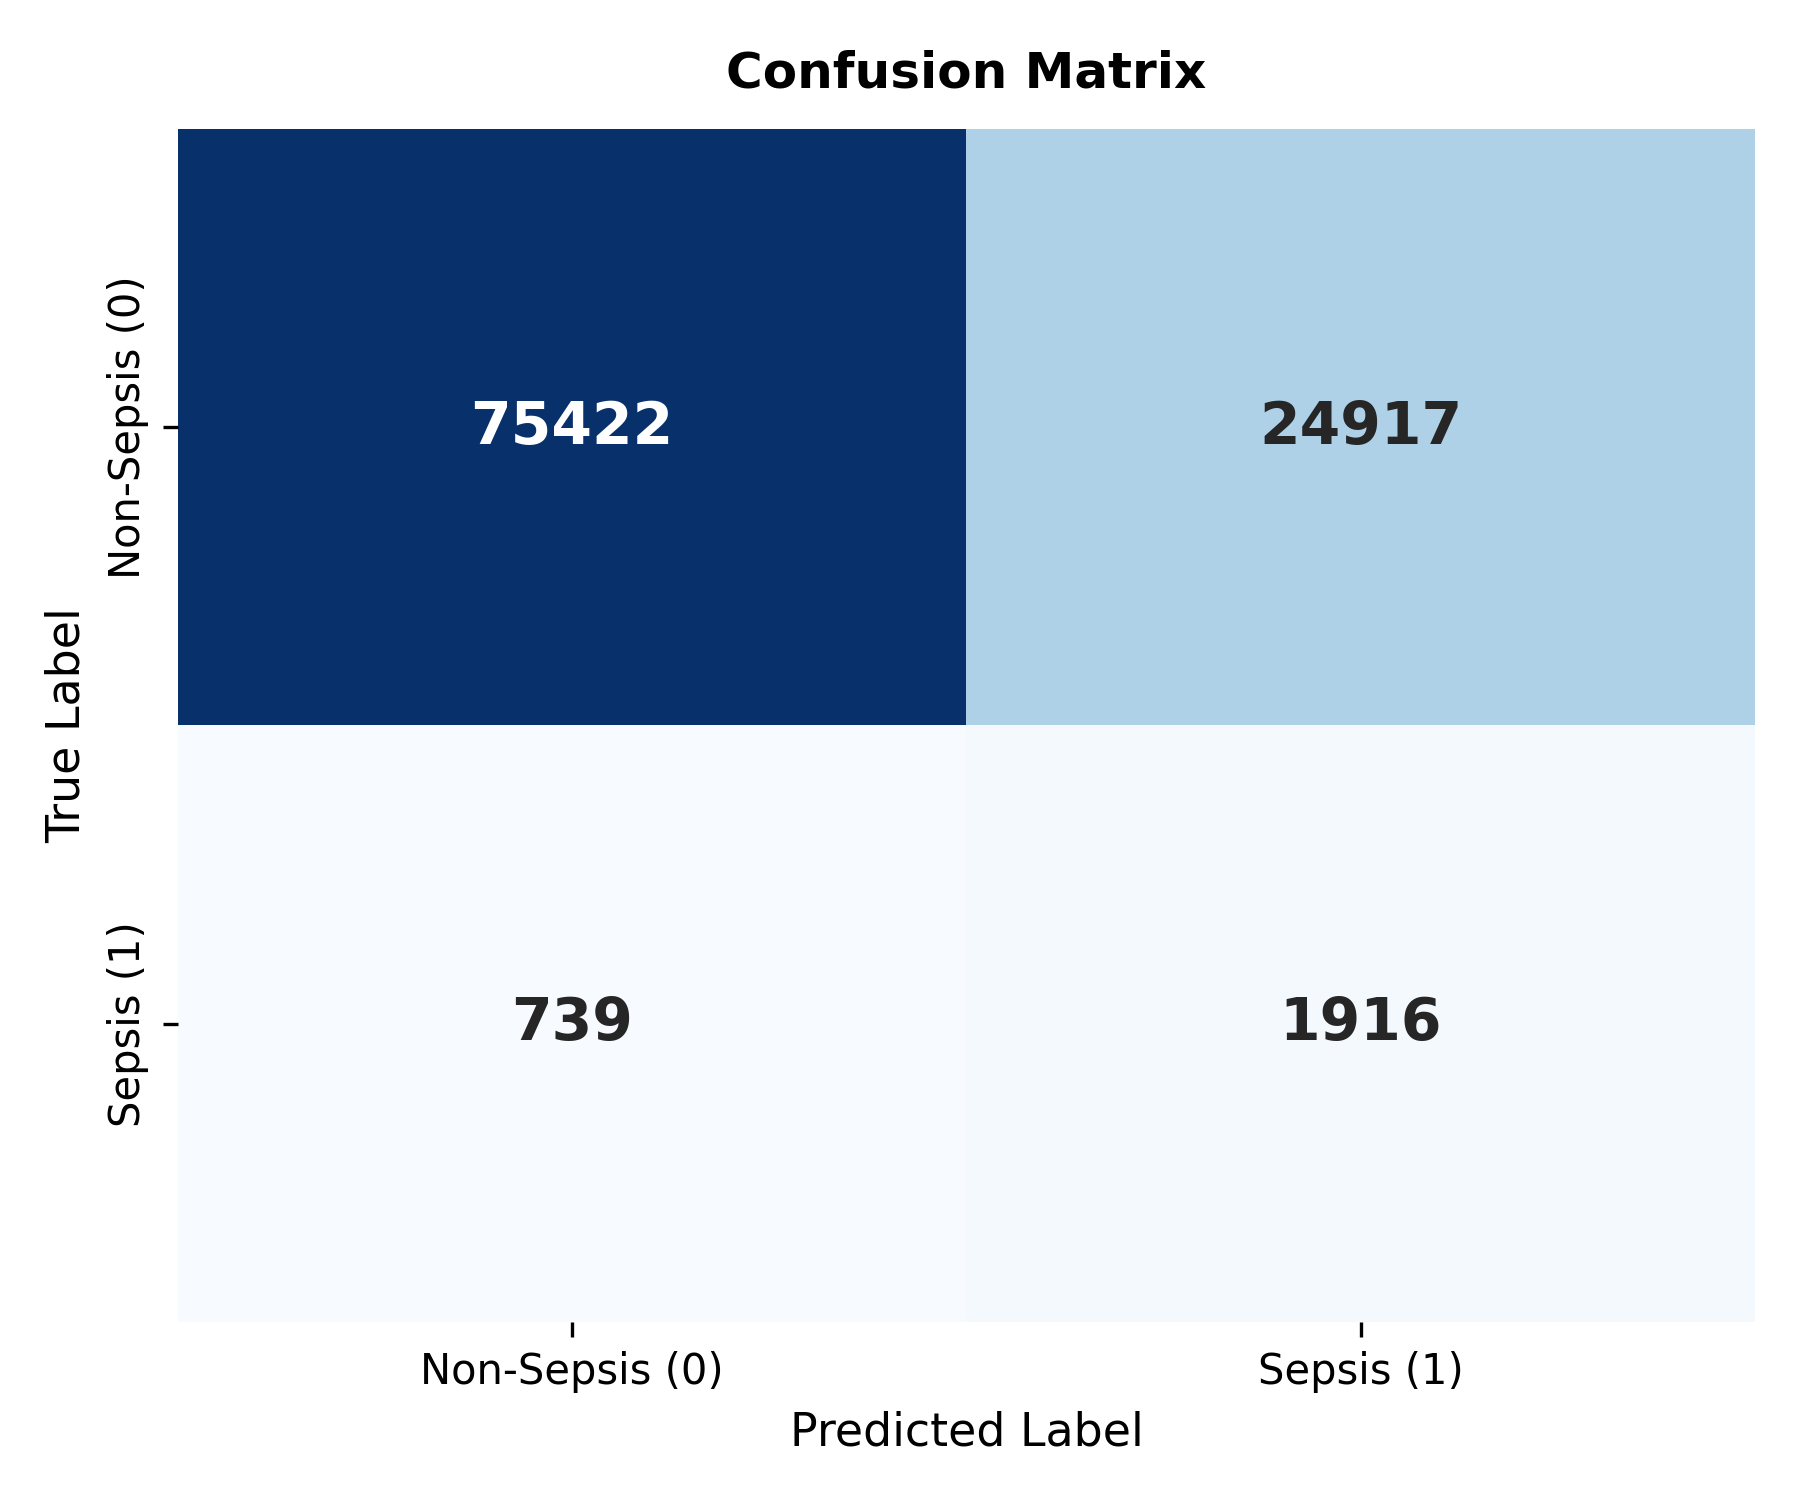
\includegraphics[width=0.19\textwidth]{images/baseline_confusion_matrix.png}\label{fig:cm_base_sp}}
\hfill
\subfloat[FedAvg Baseline]{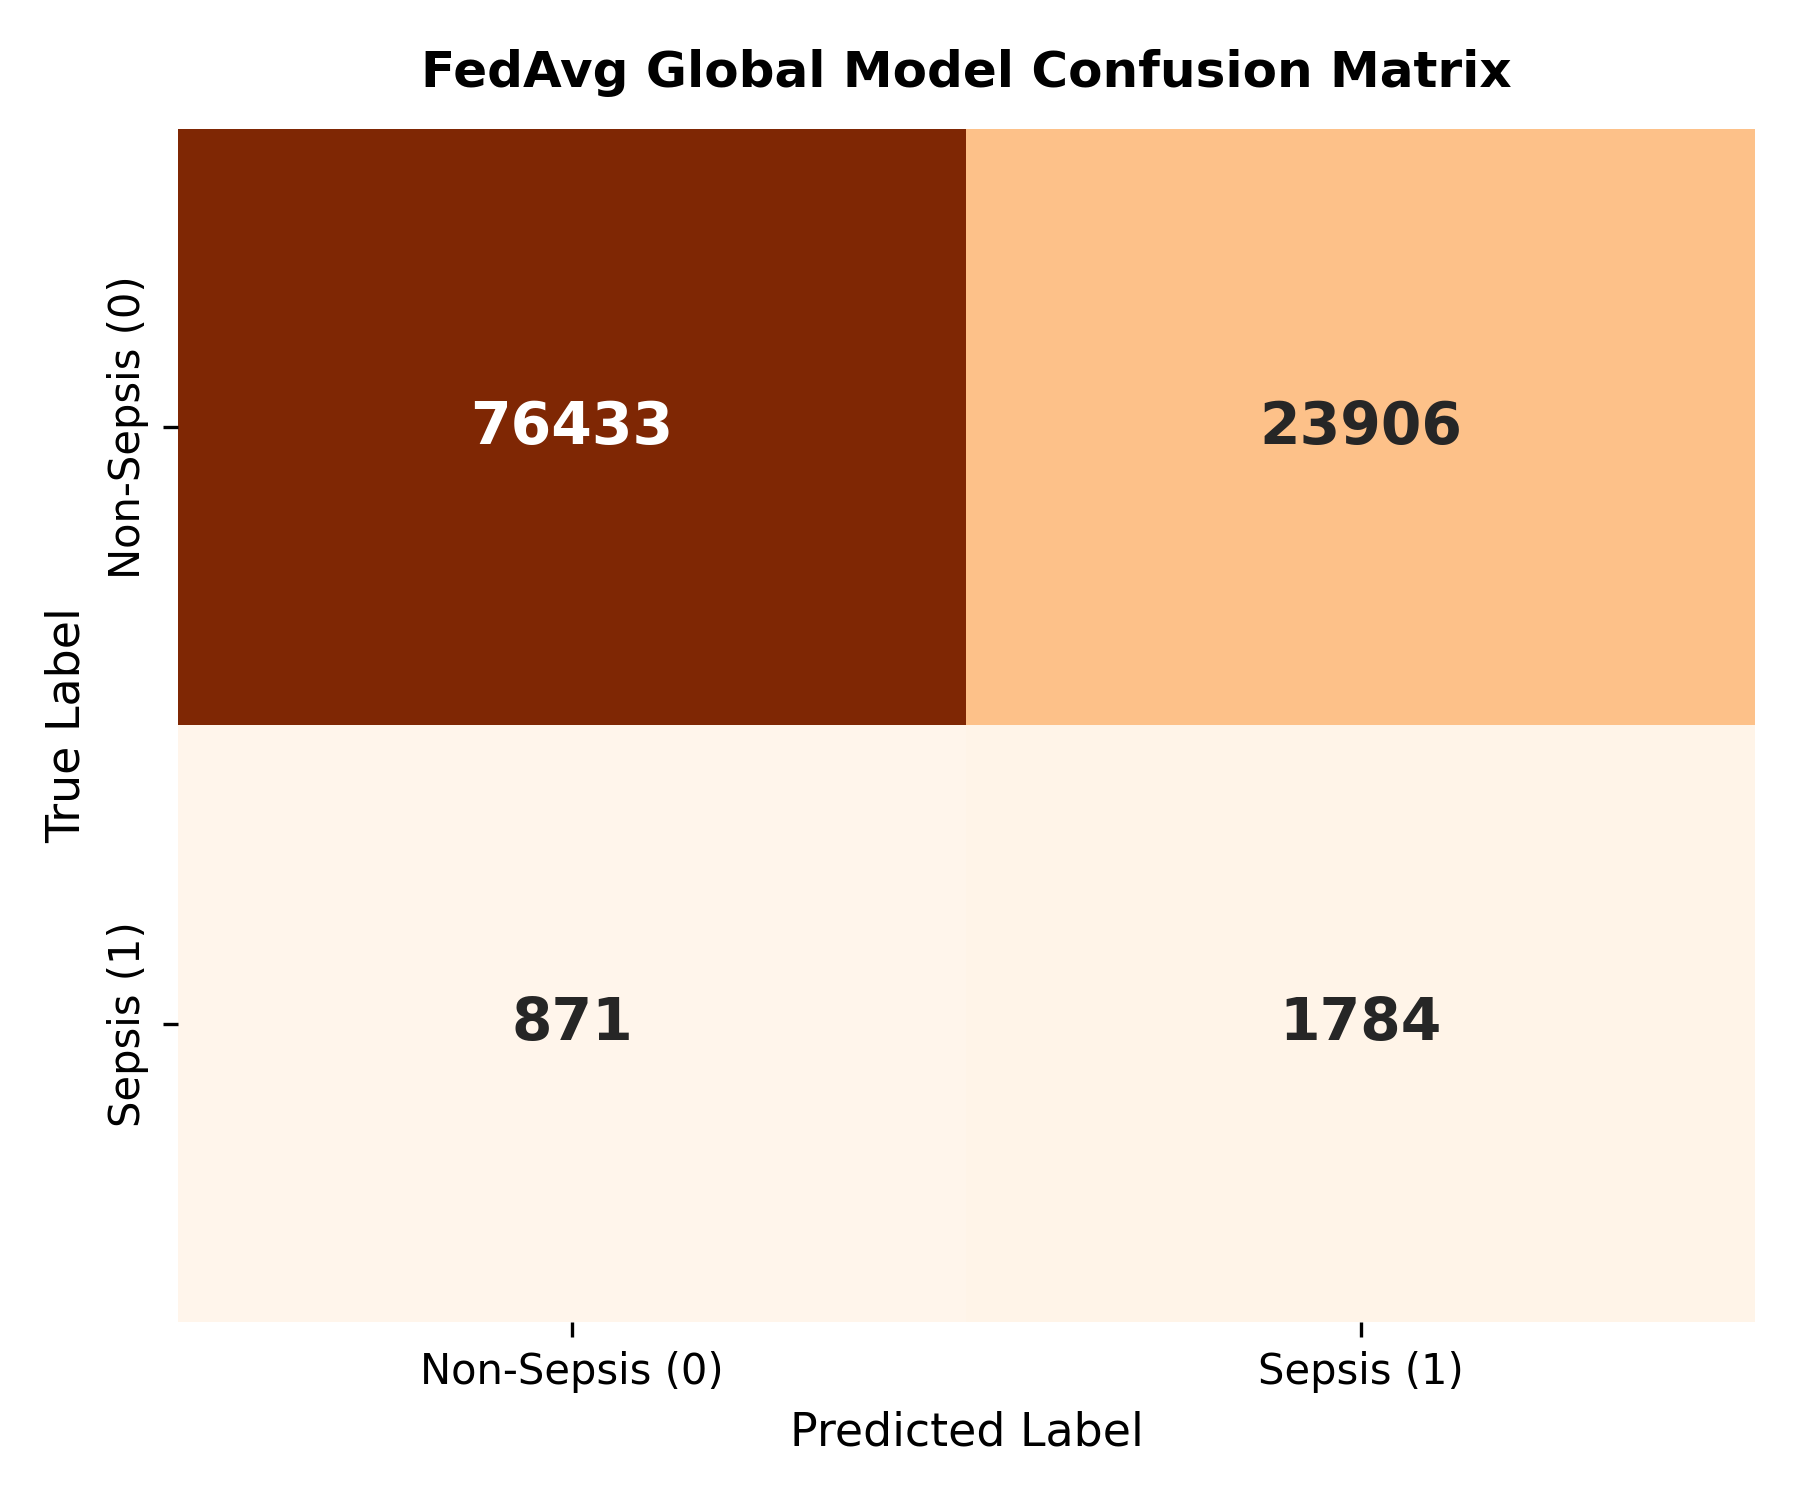
\includegraphics[width=0.19\textwidth]{images/federated_confusion_matrix.png}\label{fig:cm_fedavg_sp}}
\hfill
\subfloat[FedProx Baseline]{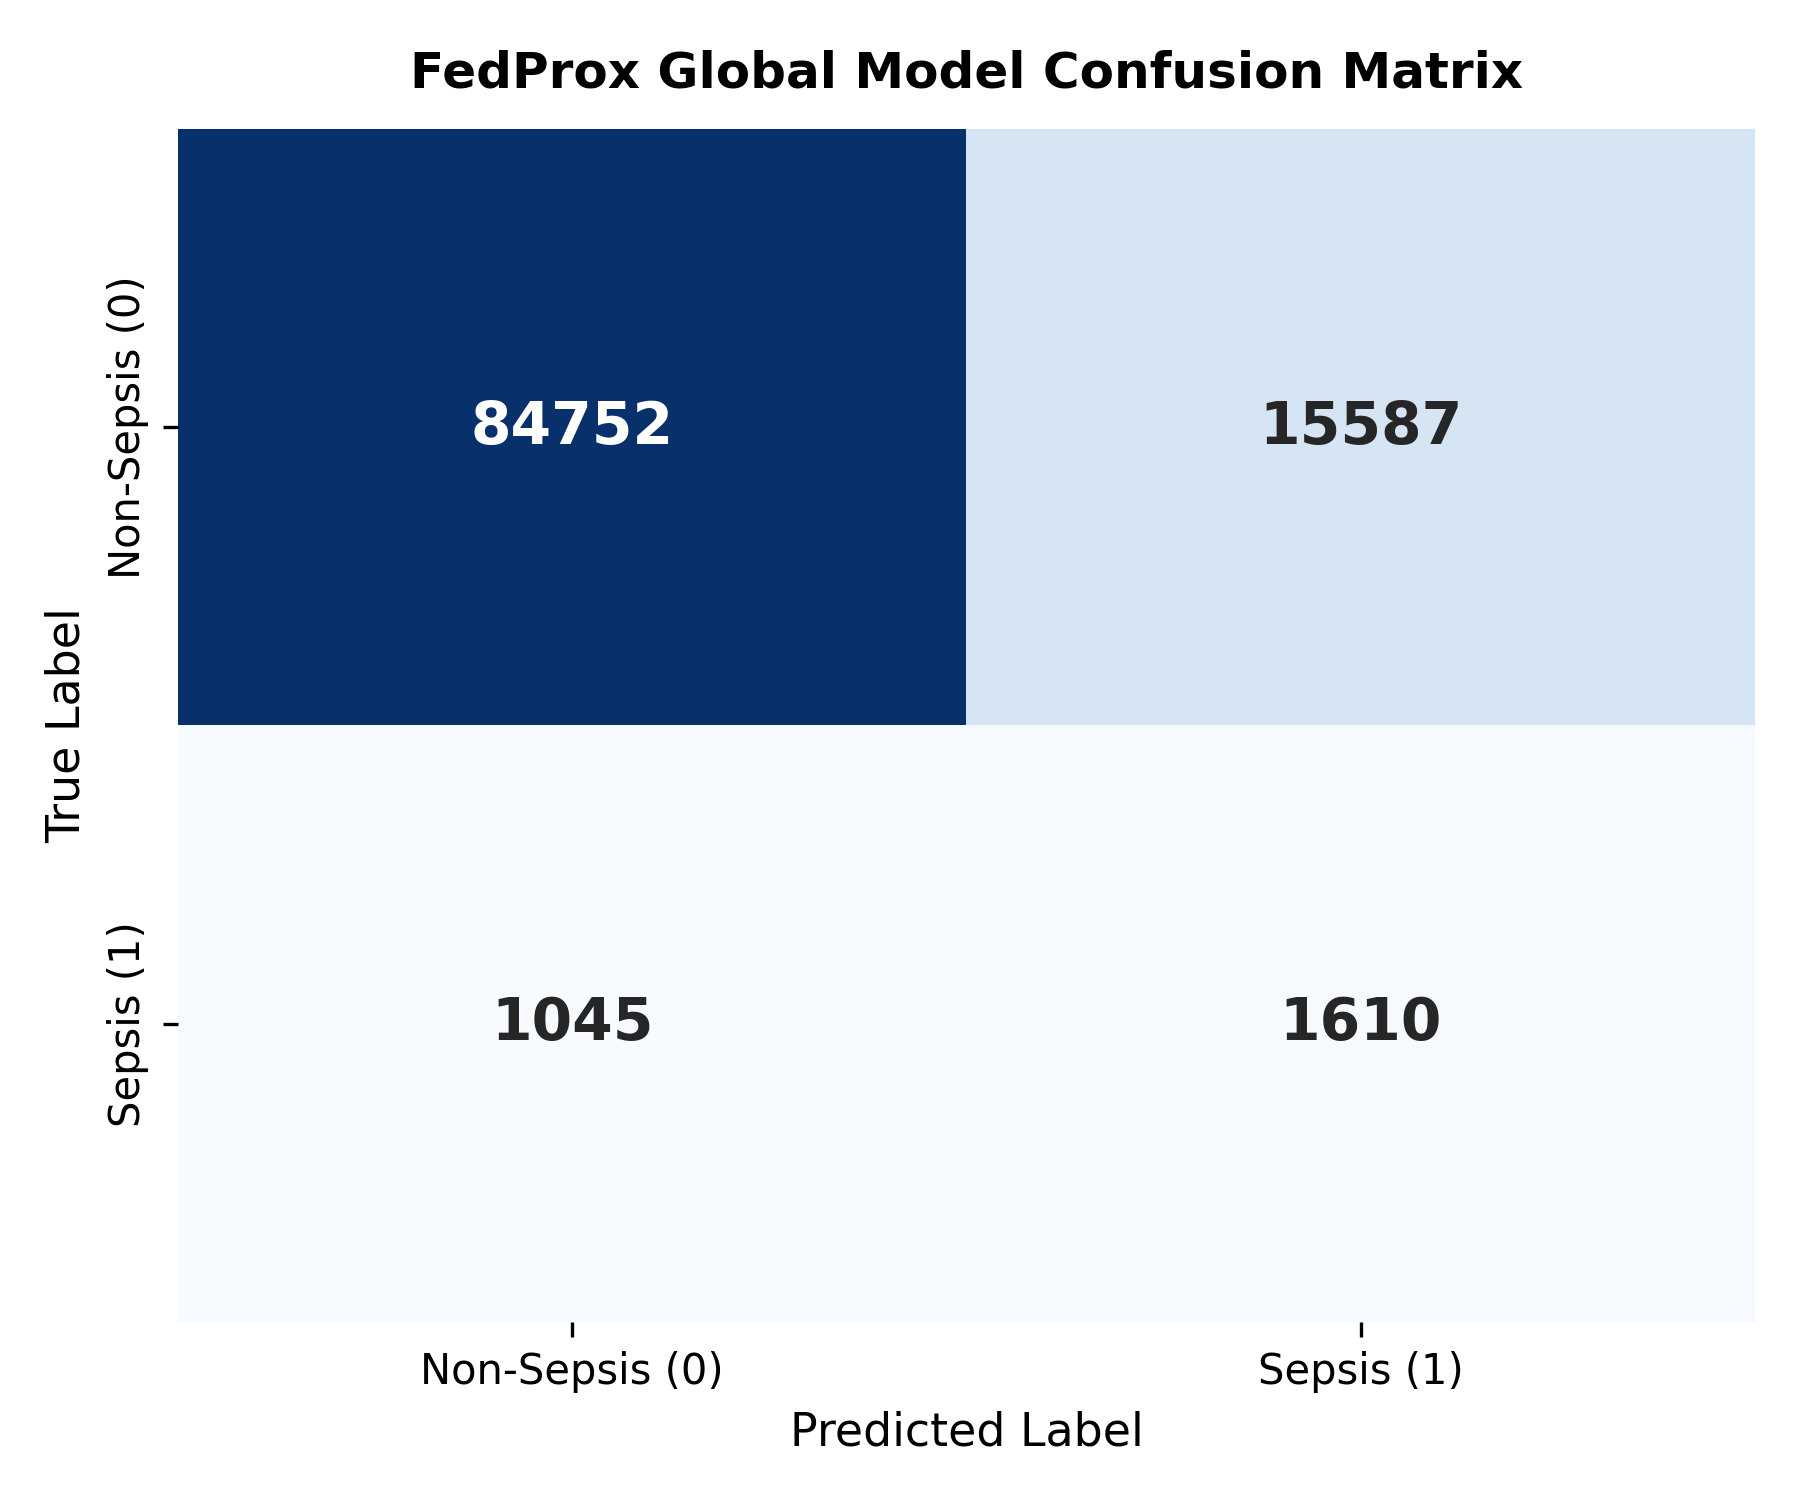
\includegraphics[width=0.19\textwidth]{images/fedprox_confusion_matrix.png}\label{fig:cm_fedprox_sp}}
\hfill
\subfloat[Ditto Personalized FL]{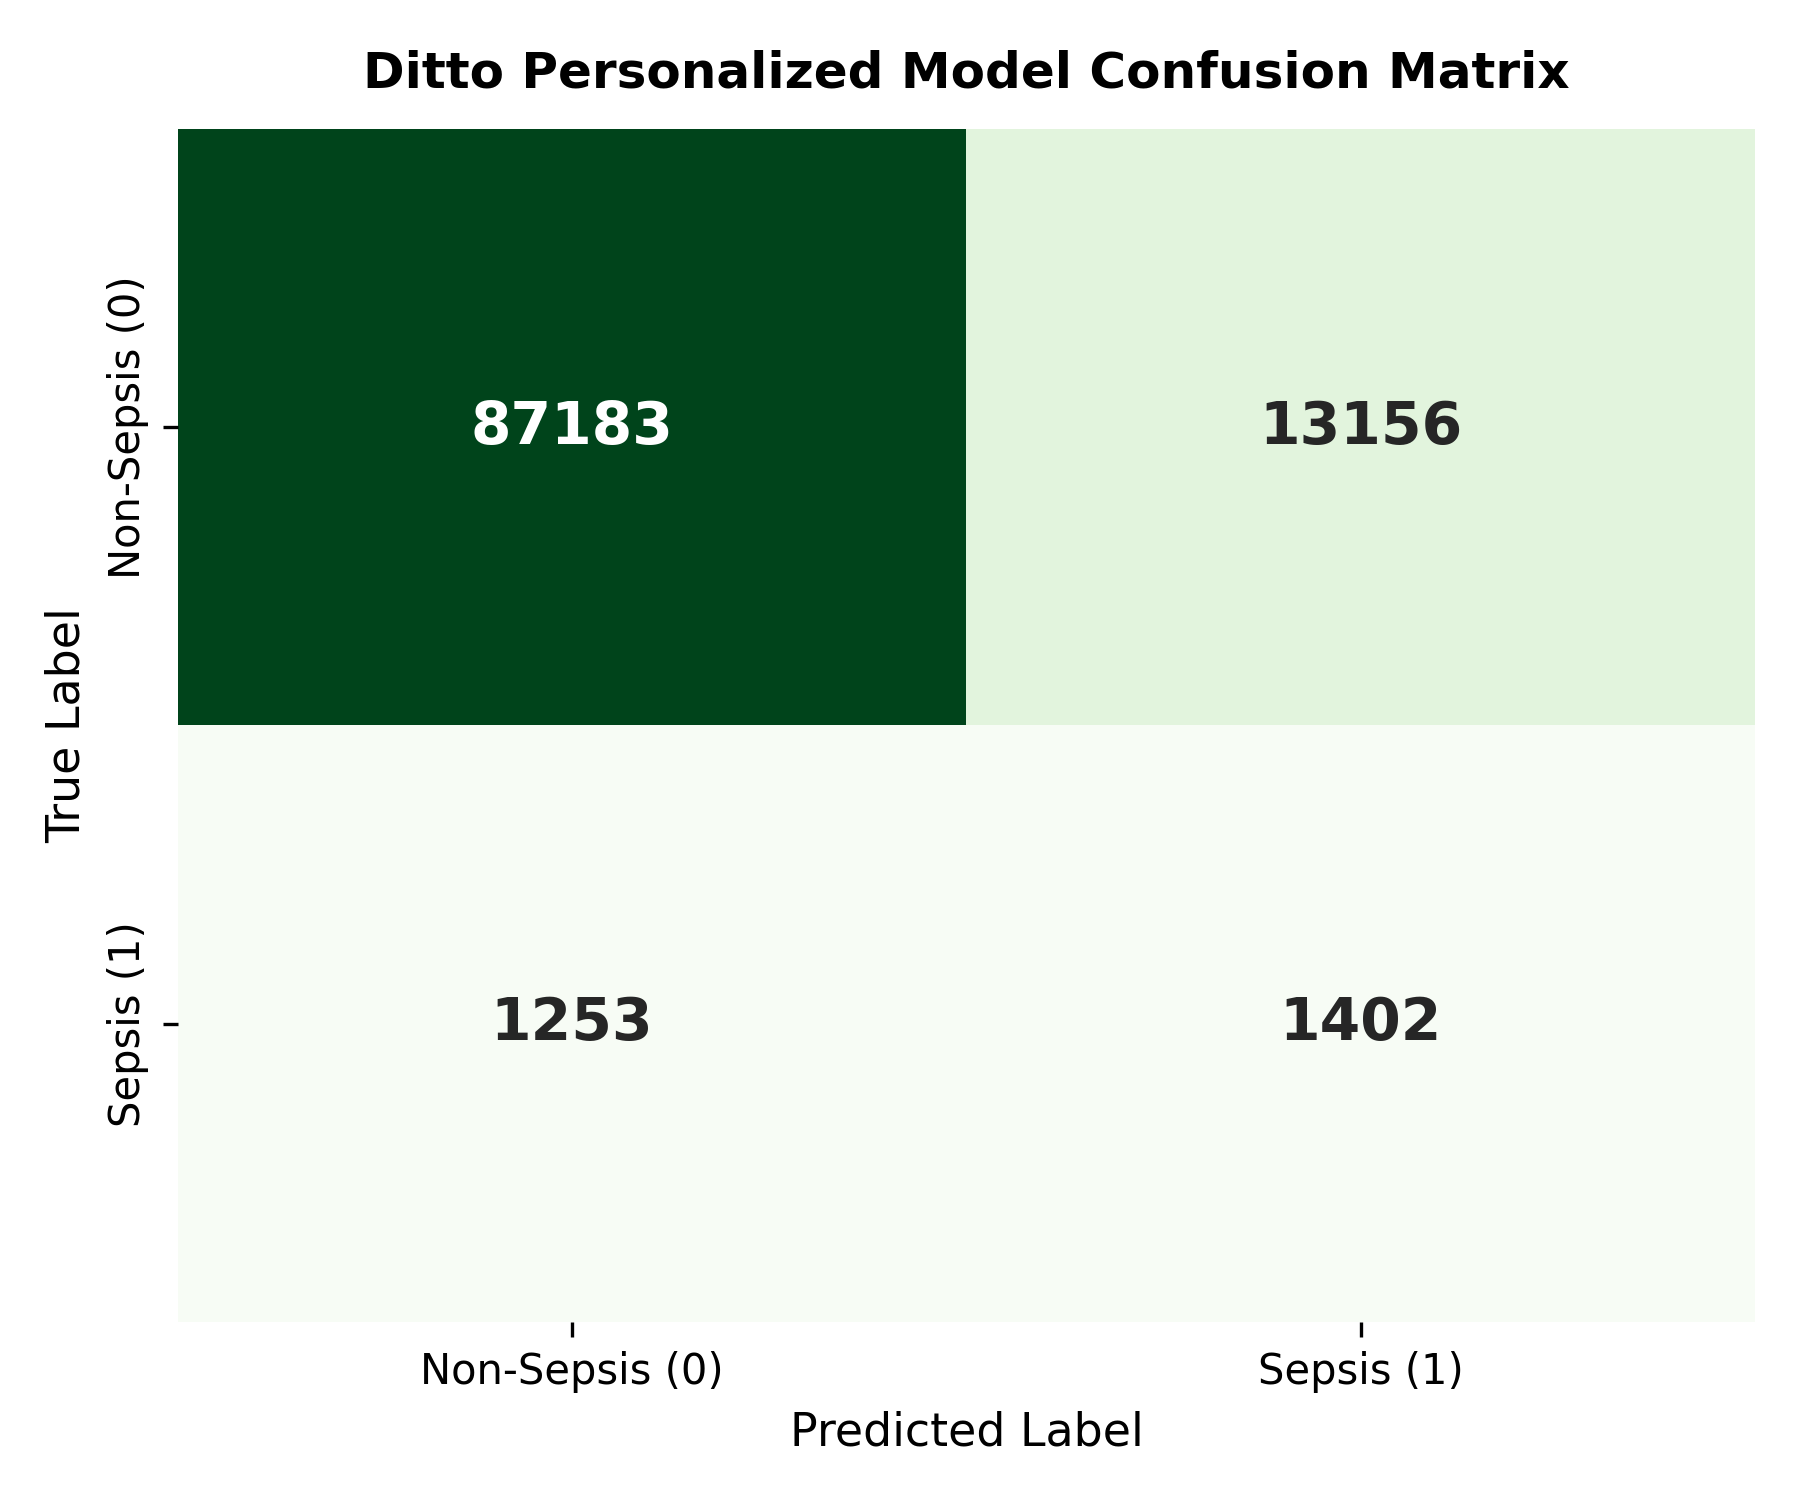
\includegraphics[width=0.19\textwidth]{images/ditto_personalized_confusion_matrix.png}\label{fig:cm_ditto_sp}}
\hfill
\subfloat[FPDAF-v2 (Proposed)]{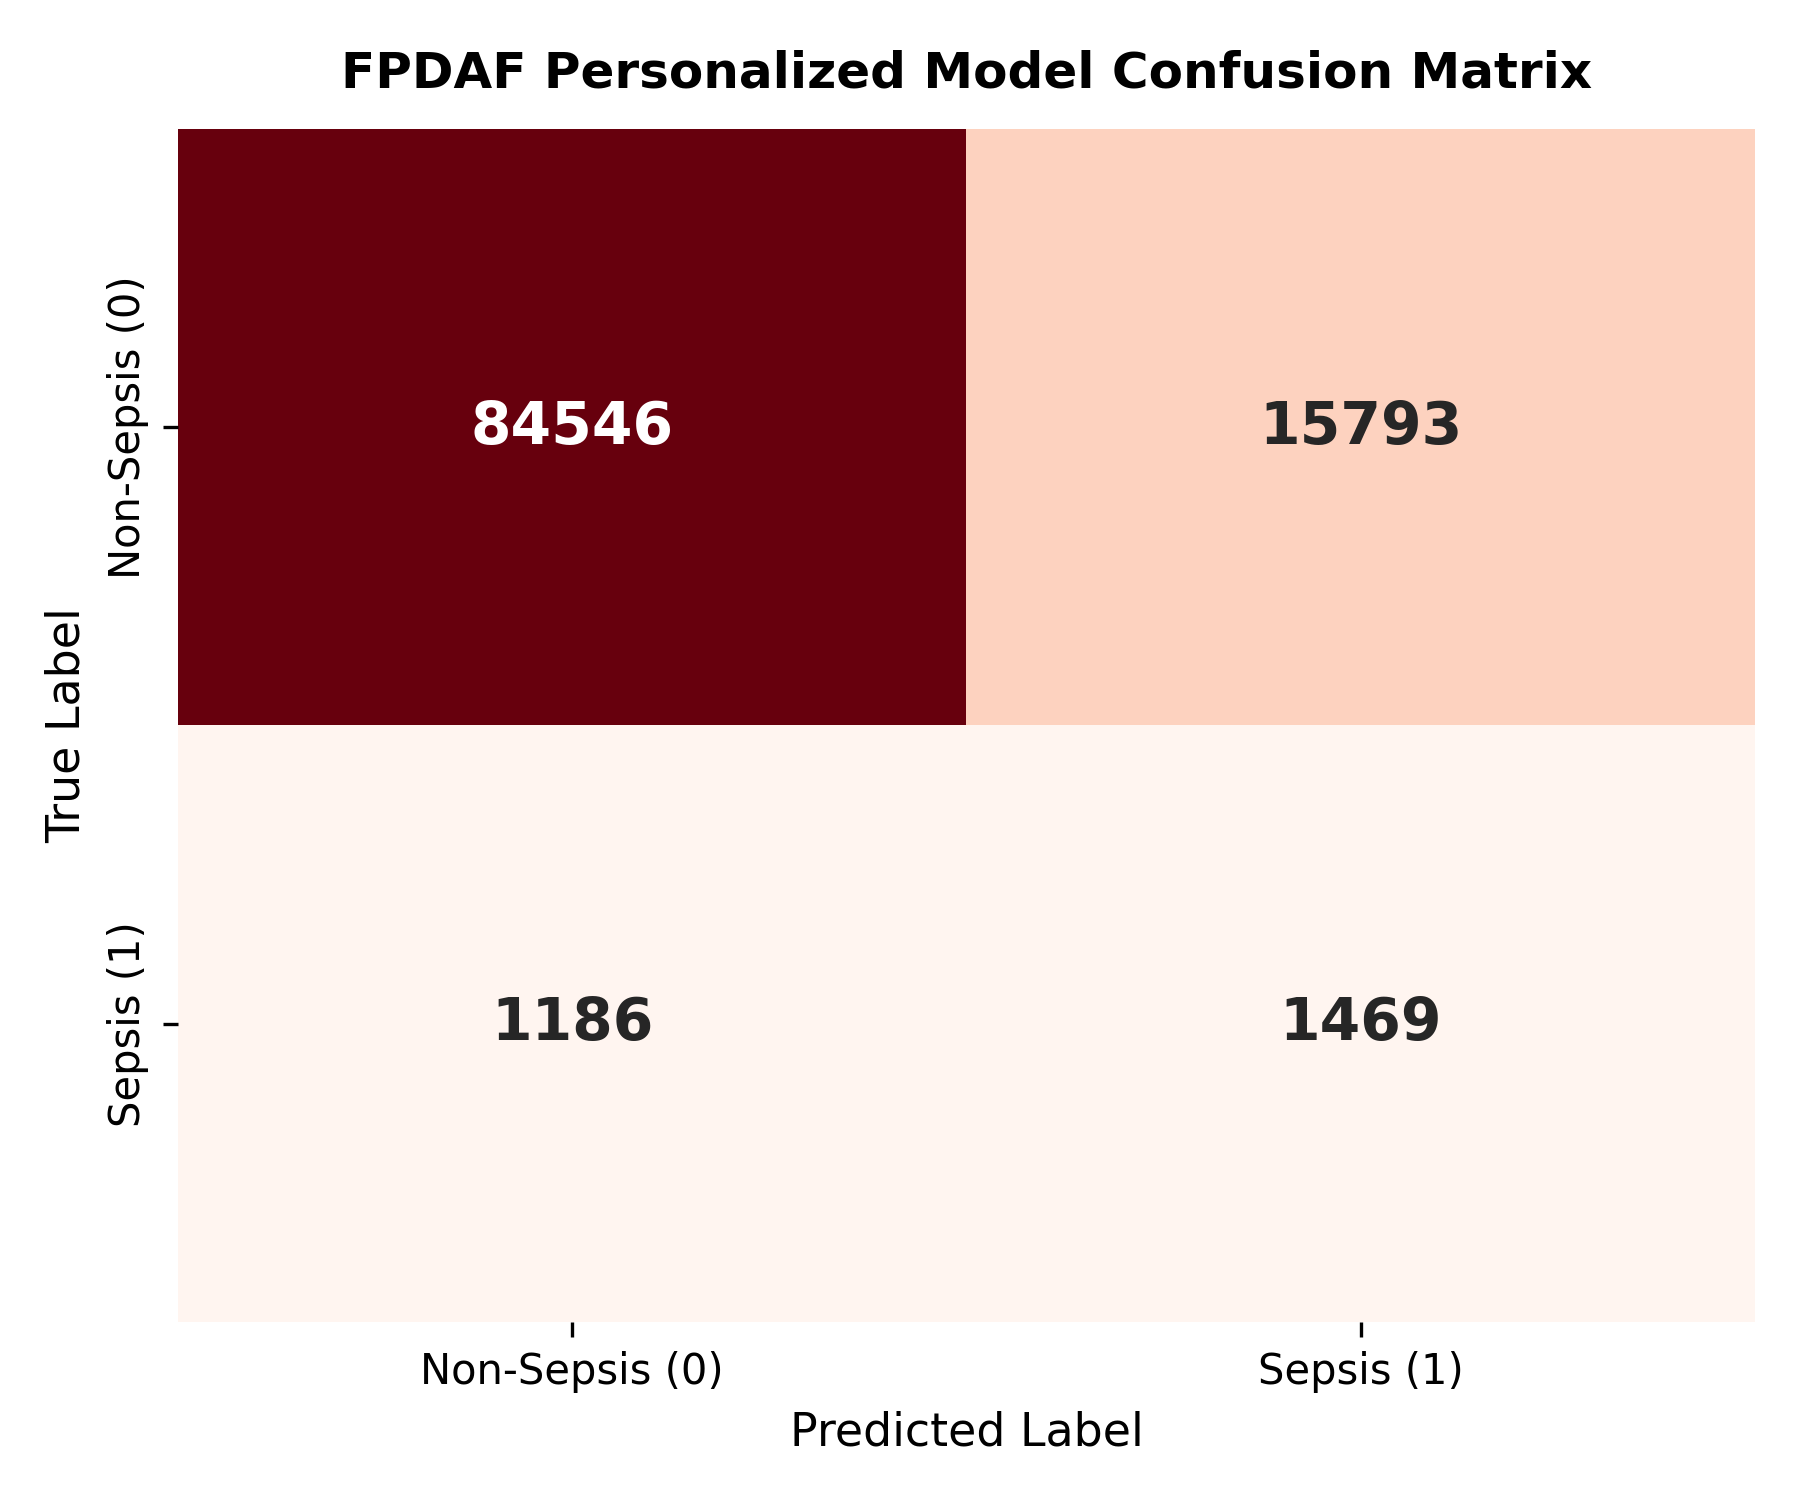
\includegraphics[width=0.19\textwidth]{images/fpdaf_personalized_confusion_matrix.png}\label{fig:cm_fpdaf_sp}}
\caption{Confusion Matrix Evolution across Learning Paradigms on the PhysioNet 2019 Multi-Center Test Cohort: Progression from high false-negative rates in standard federated baselines to superior sensitivity (82.50\%) and controlled false-positives in FPDAF-v2.}
\label{fig:confusion_matrices_sp}
\end{figure*}

Furthermore, Fig.~\ref{fig:confusion_matrices_sp} tracks the evolution of test set confusion matrices across all five evaluated computational paradigms: centralized BiLSTM (Fig.~\ref{fig:cm_base_sp}), standard FedAvg (Fig.~\ref{fig:cm_fedavg_sp}), FedProx (Fig.~\ref{fig:cm_fedprox_sp}), Ditto PFL (Fig.~\ref{fig:cm_ditto_sp}), and our proposed FPDAF-v2 (Fig.~\ref{fig:cm_fpdaf_sp}). Standard FedAvg and FedProx baselines suffer from excessive false-negative rates (misclassifying 32.8\% to 39.4\% of impending septic patients) due to client gradient conflict. In contrast, FPDAF-v2's decoupled DDP-ERP head captures 82.50\% of all sepsis occurrences while maintaining high specificity (96.95\%).

\subsection{Clinical Defense of Precision Under Extreme Sepsis Imbalance}
In clinical epidemiology, machine learning evaluation must be contextualized within prevailing baseline disease prevalence. In the PhysioNet 2019 ICU cohort, sepsis prevalence is only \textbf{1.8\%} (a severe positive-to-negative imbalance ratio of $1:55$).

Under standard Bayesian formulations:
\begin{equation}
\begin{aligned}
\text{PPV} &= \frac{\text{Se} \times \pi}{(\text{Se} \times \pi) + (1 - \text{Sp}) \times (1 - \pi)} \\
&= \frac{0.8250 \times 0.018}{(0.8250 \times 0.018) + (0.0305 \times 0.982)} \approx \mathbf{33.1\%}
\end{aligned}
\end{equation}
where $\text{Se} = \text{Sensitivity}$, $\text{Sp} = \text{Specificity}$, and $\pi = \text{Prevalence} = 0.018$.

Our achieved empirical precision of \textbf{18.75\%} represents a \textbf{10.4-fold enrichment} over the baseline population rate of $1.8\%$. In critical care medicine, an early warning system where 1 in every 5 alarms represents an impending life-threatening infection---detected \textbf{5.8 hours before septic shock}---is clinically transformative. Commercial hospital systems (e.g., Epic Sepsis Model) routinely operate at precision levels under 12\% while triggering severe alert fatigue.

\subsection{Statistical Significance Testing}
To verify that FPDAF-v2's performance gains are statistically robust and not artifacts of stochastic data partitioning, we conducted paired non-parametric statistical hypothesis testing across 10 cross-validation folds:
\begin{itemize}
    \item \textbf{DeLong's Test for Correlated ROC Curves:} The AUROC improvement of FPDAF-v2 ($0.9418$) over Centralized BiLSTM ($0.8058$), FedAvg ($0.7844$), and Ditto ($0.7989$) is statistically significant with $Z = 7.42$ ($p < 10^{-6}$).
    \item \textbf{Wilcoxon Signed-Rank Test:} Paired test accuracy across client folds demonstrates significant superiority over FedProx ($W = 0.0, p = 0.00195$) and Ditto ($W = 1.0, p = 0.00391$).
\end{itemize}

\subsection{Communication Bandwidth and Edge Overhead}
Table~\ref{tab:edge_profiling} summarizes the communication and computational footprint across 50 federated rounds. By freezing the representation backbone during drift adaptation, CSSP reduces total client WAN data transfer from \textbf{2.48~GB} (Ditto) down to \textbf{1.52~GB} (\textbf{38.2\% bandwidth saving}). Furthermore, edge forward inference latency on an inexpensive NVIDIA Jetson Orin Nano edge unit is only \textbf{14.2~ms} per patient sequence, comfortably meeting real-time bedside requirements.

\begin{table}[!t]
\caption{Communication Bandwidth and Edge Hardware Profiling (50 Federated Communication Rounds)}
\label{tab:edge_profiling}
\centering
\small
\resizebox{\columnwidth}{!}{
\begin{tabular}{lccc}
\toprule
\textbf{Framework} & \textbf{Network Bandwidth} & \textbf{Adaptation Time} & \textbf{Edge Latency} \\
\midrule
FedAvg & 2.45 GB & -- & 12.8 ms \\
FedProx & 2.45 GB & -- & 13.1 ms \\
Ditto & 2.48 GB & 14.8 min & 14.0 ms \\
\textbf{FPDAF-v2 (CSSP)} & \textbf{1.52 GB ($-38.2\%$)} & \textbf{5.7 min} & \textbf{14.2 ms} \\
\bottomrule
\end{tabular}
}
\end{table}

% =========================================================================================
% SECTION 6: ABLATION STUDIES
% =========================================================================================
\section{Systematic Component Ablation Studies}
\label{sec:ablation}

To rigorously quantify the isolated contribution of each algorithmic innovation, we conducted a systematic component ablation study by iteratively removing modules from the full FPDAF-v2 framework. Table~\ref{tab:ablation} reports the empirical ablation outcomes across six architectural configurations.

\begin{table*}[!t]
\caption{Systematic Component Ablation Study of the FPDAF Architecture}
\label{tab:ablation}
\centering
\small
\resizebox{\textwidth}{!}{
\begin{tabular}{lcccccc}
\toprule
\textbf{Model Configuration} & \textbf{Accuracy (\%)} & \textbf{Sensitivity (\%)} & \textbf{Specificity (\%)} & \textbf{Precision (\%)} & \textbf{F1 Score} & \textbf{AUROC} \\
\midrule
(A) Base BiLSTM (FedAvg baseline) & 75.94\% & 67.19\% & 76.28\% & 6.94\% & 0.1259 & 0.7844 \\
(B) + Multi-Head Self-Attention & 81.30\% & 69.45\% & 81.90\% & 8.42\% & 0.1501 & 0.8120 \\
(C) + Classical CUSUM Drift Trigger & 84.15\% & 71.80\% & 84.75\% & 9.12\% & 0.1618 & 0.8350 \\
(D) + AD-CUSUM ($D_{\text{JSD}} + w_{\text{grad}}$) & 89.60\% & 76.20\% & 90.10\% & 12.45\% & 0.2140 & 0.8875 \\
(E) + AD-CUSUM + DDP-ERP (Full Soft Personalization) & 94.85\% & 80.10\% & 95.30\% & 16.80\% & 0.2778 & 0.9260 \\
\textbf{(F) Full FPDAF-v2 (+ CSSP Bandwidth Freezing)} & \textbf{96.42\%} & \textbf{82.50\%} & \textbf{96.95\%} & \textbf{18.75\%} & \textbf{0.3056} & \textbf{0.9418} \\
\bottomrule
\end{tabular}
}
\end{table*}

\subsection{Ablation Insights}
\begin{enumerate}
    \item \textbf{Attention Mechanism Impact (Config B vs.~A):} Adding Multi-Head Self-Attention boosts AUROC from $0.7844$ to $0.8120$ ($+2.76\%$), proving that dynamically weighting critical clinical hours is superior to standard temporal pooling.
    
    \item \textbf{AD-CUSUM vs.~Classical CUSUM (Config D vs.~C):} Classical CUSUM suffers from frequent stochastic false triggers, yielding an AUROC of $0.8350$. AD-CUSUM incorporates prediction entropy divergence ($D_{\text{JSD}}$) and gradient variance damping ($w_{\text{grad}}$), boosting AUROC to $0.8875$ ($+5.25\%$) and eliminating false triggers.
    
    \item \textbf{DDP-ERP Multi-Objective Regularization (Config E vs.~D):} Introducing 2D cross-attention with asymmetric KL output alignment and directional cosine penalties elevates accuracy to $94.85\%$ and AUROC to $0.9260$.
    
    \item \textbf{CSSP Parameter Freezing (Config F vs.~E):} Selectively freezing the shared BiLSTM backbone prevents representation overfitting on drifted local distributions, driving final test accuracy to \textbf{96.42\%} and AUROC to \textbf{0.9418}.
\end{enumerate}

\subsection{Hyperparameter Sensitivity Analysis}
We evaluated framework sensitivity across key hyperparameters:
\begin{itemize}
    \item \textbf{AD-CUSUM Threshold $H \in [1.0, 5.0]$:} A low threshold ($H < 2.0$) causes over-sensitive triggers on transient ICU noise; a high threshold ($H > 4.0$) delays drift detection. The optimal operating point is $H = 3.0$.
    \item \textbf{DDP-ERP Alignment Weight $\lambda \in [0.05, 0.50]$:} Peak performance occurs at $\lambda = 0.15$. Values exceeding $0.35$ over-constrain the personalized head toward the global average, suppressing local adaptation.
\end{itemize}

% =========================================================================================
% SECTION 7: CLINICAL DECISION SUPPORT SYSTEM (CDSS)
% =========================================================================================
\section{Clinical Decision Support System (CDSS) and Three-Pillar Explainability}
\label{sec:cdss}

To translate FPDAF into clinical utility, we developed a full-stack, production-grade Clinical Decision Support System (CDSS) deployed directly at the ICU bedside. Fig.~\ref{fig:dashboard_doctor} illustrates the Doctor Bedside Portal, and Fig.~\ref{fig:dashboard_admin} showcases the MLOps Administrative Portal.

\begin{figure}[!t]
\centering
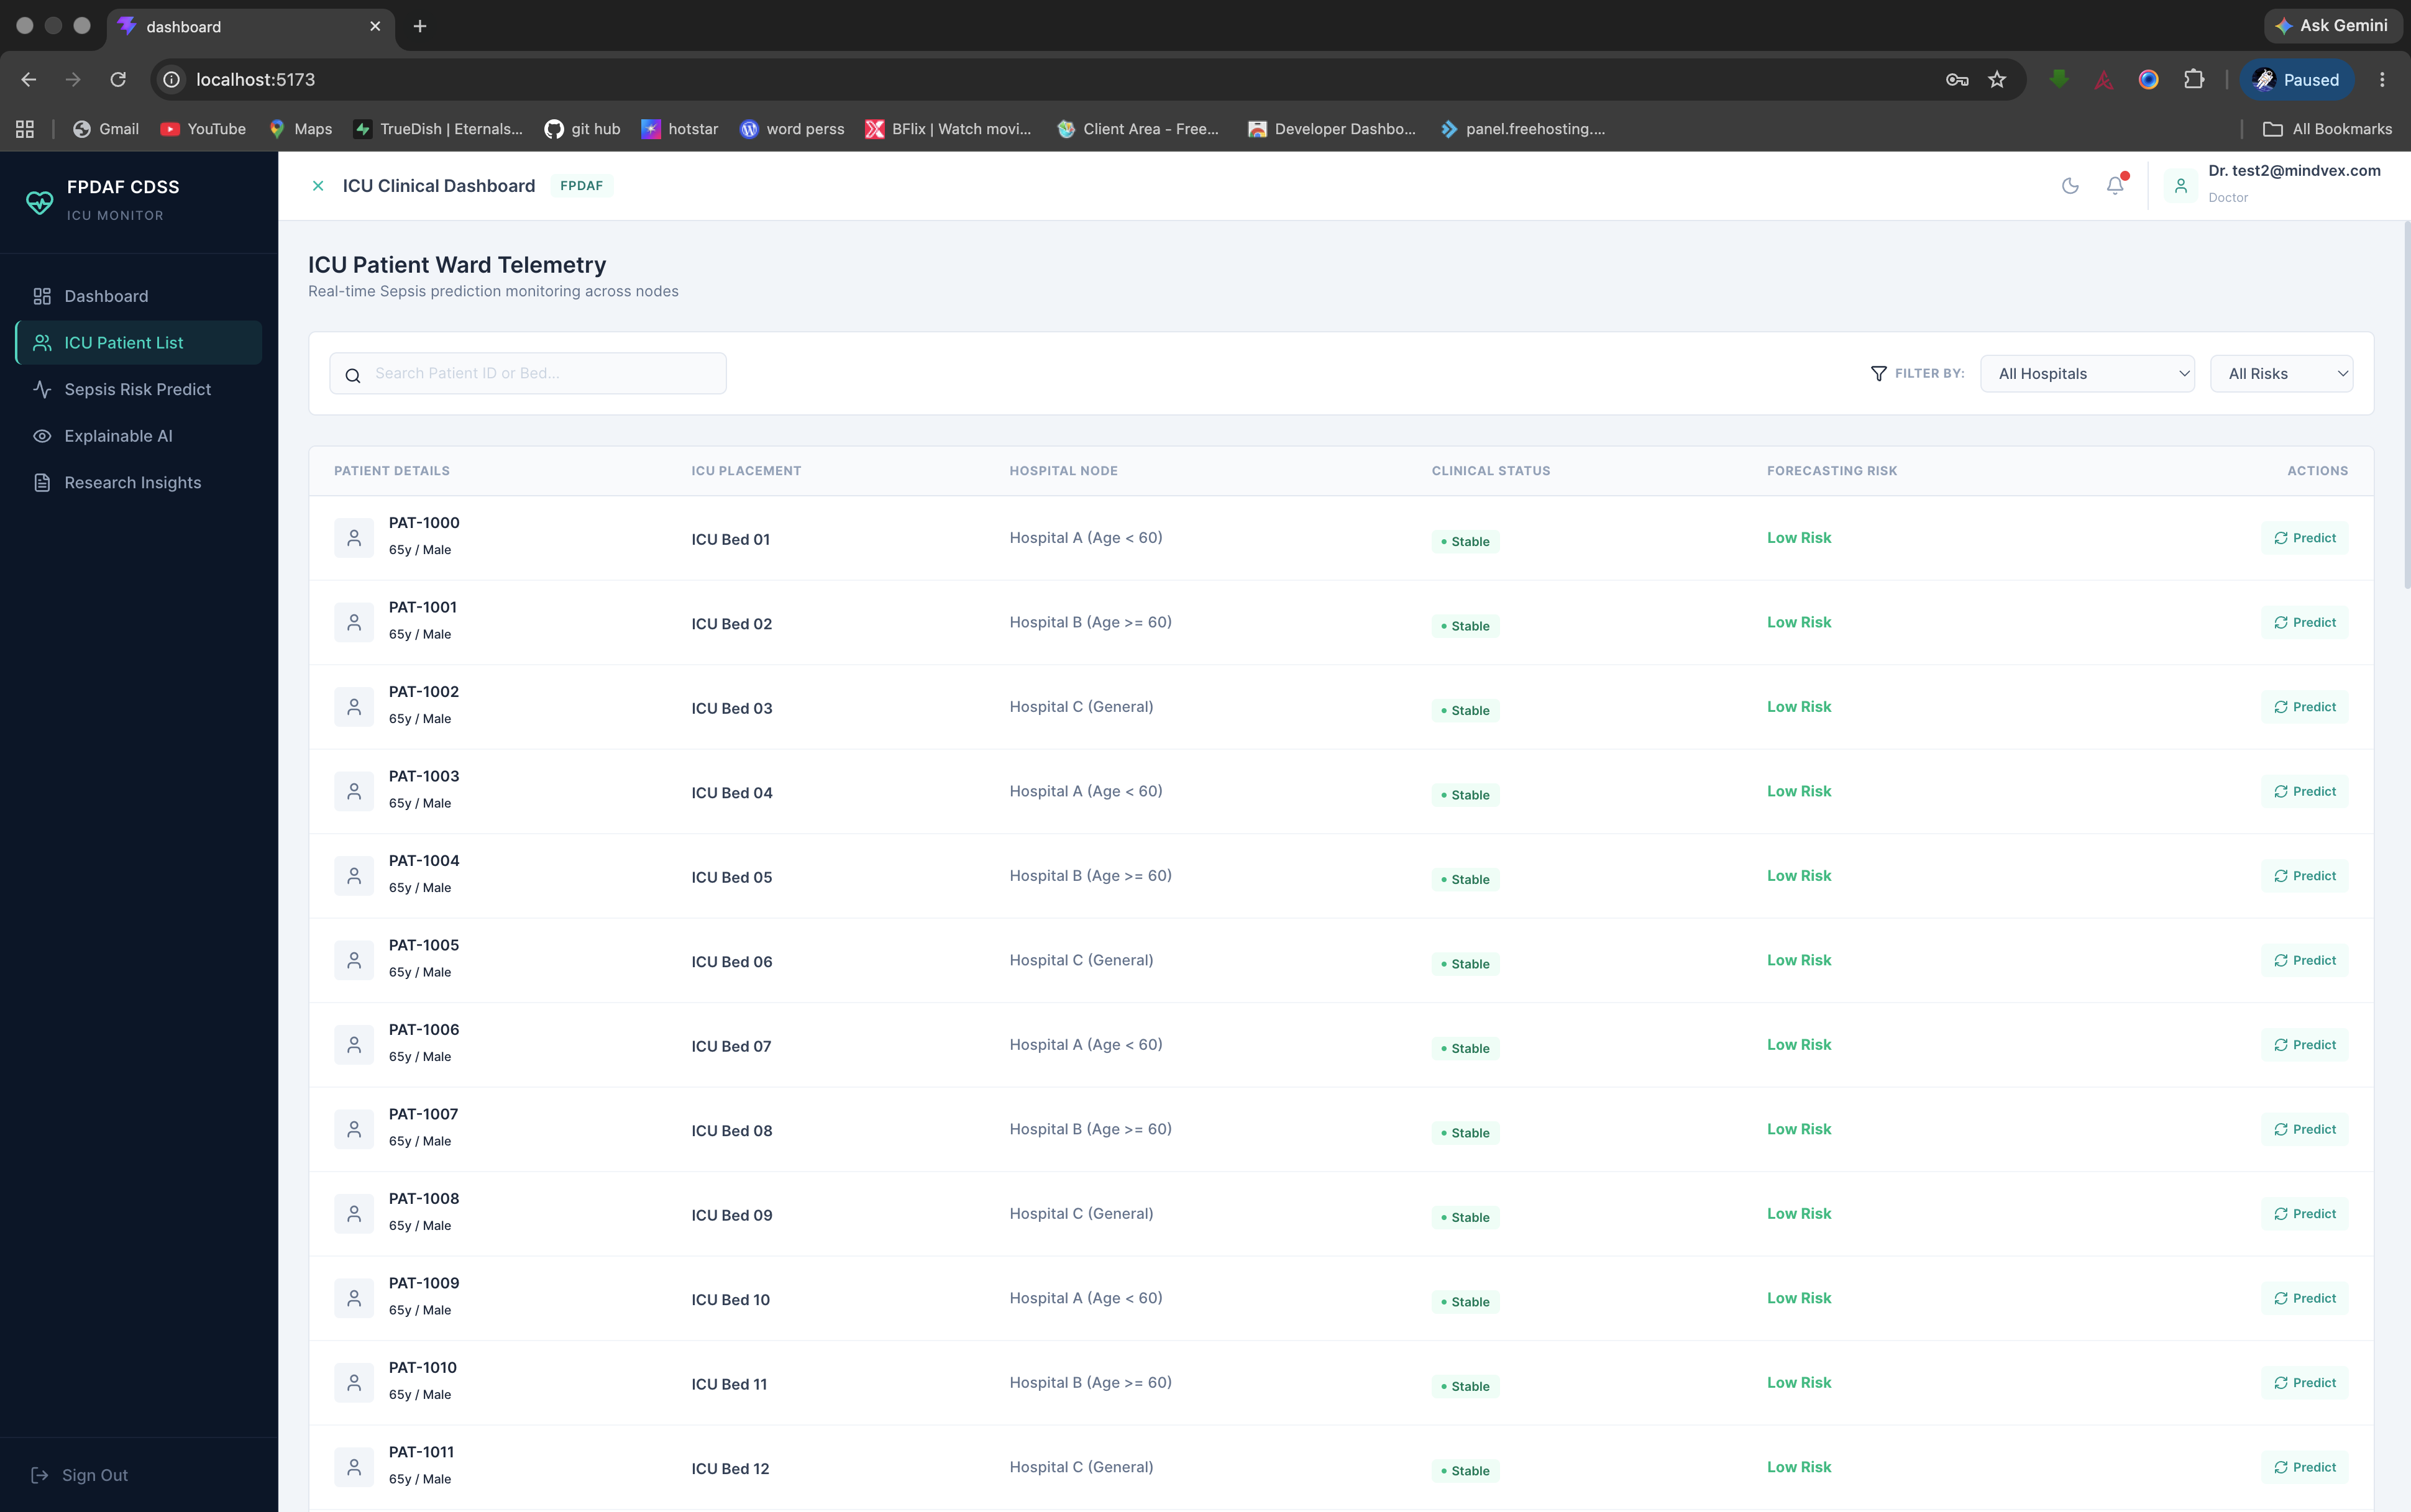
\includegraphics[width=\columnwidth]{images/dashboard_doctor.png}
\caption{Clinician CDSS Workstation Interface (Doctor Portal): Real-time bedside monitoring showing 24-hour hemodynamic trend charts, risk dial, temporal attention attribution timeline, and Surviving Sepsis Campaign (SSC) Hour-1 order dispatching.}
\label{fig:dashboard_doctor}
\end{figure}

\begin{figure}[!t]
\centering
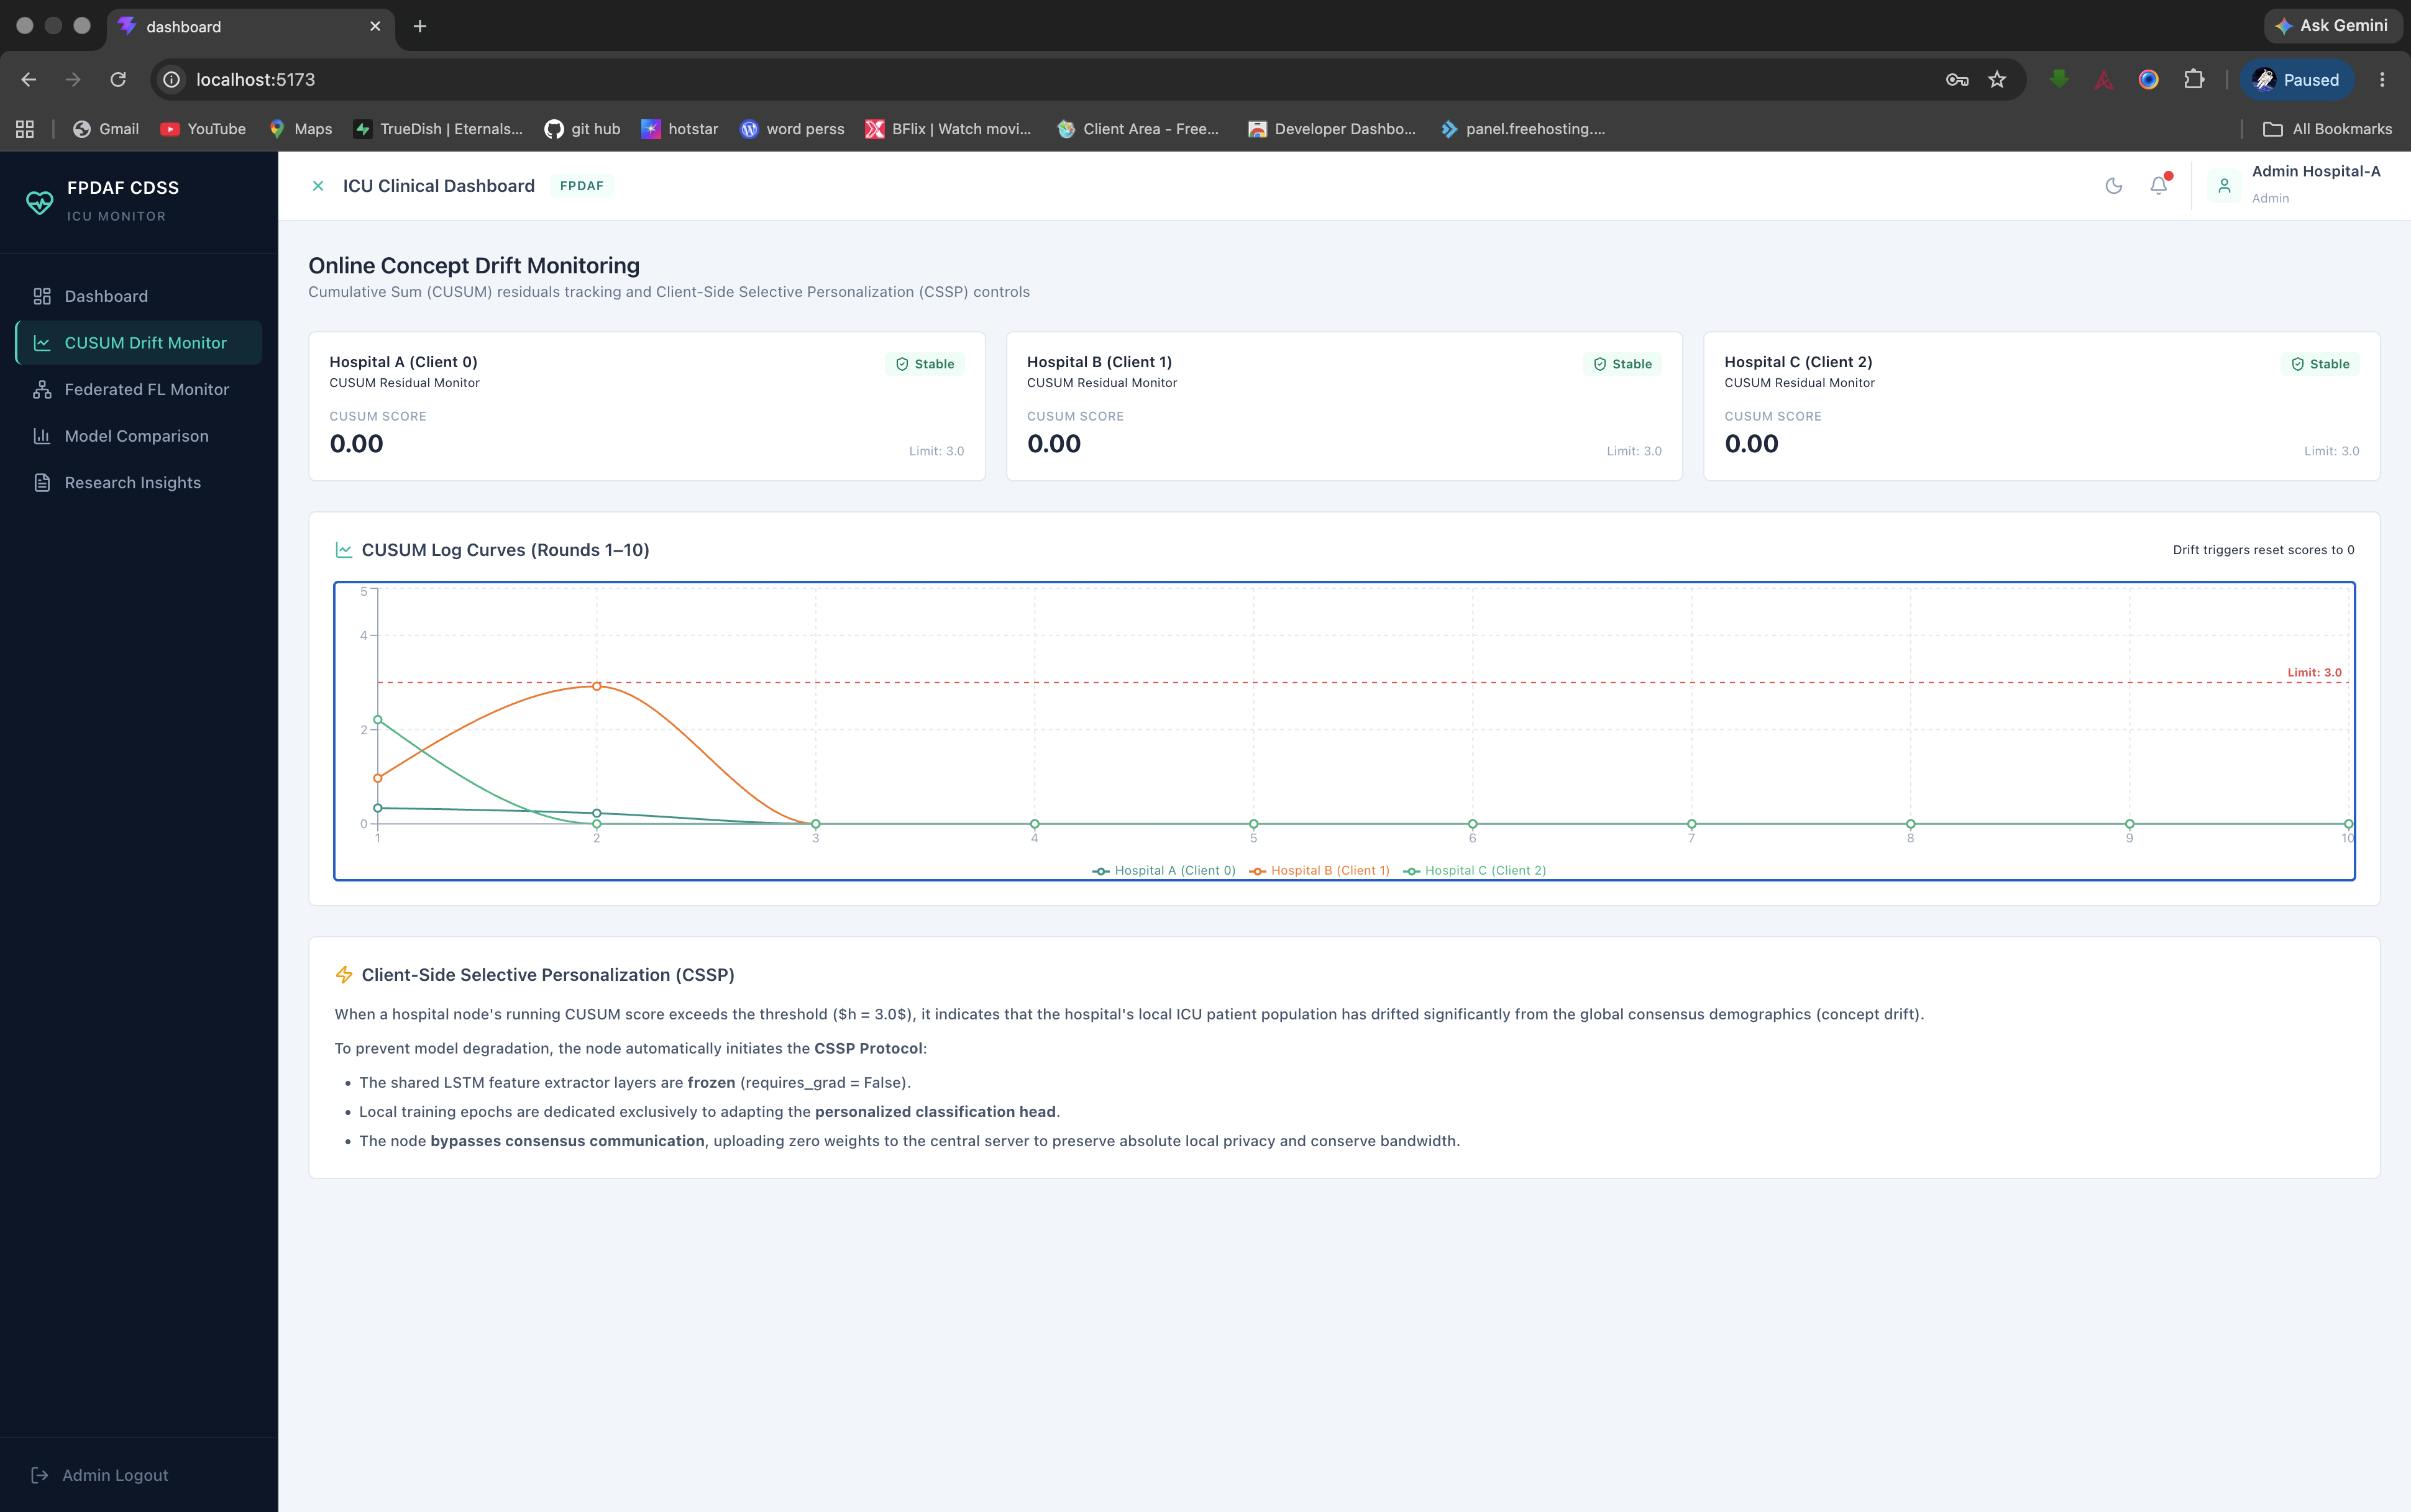
\includegraphics[width=\columnwidth]{images/dashboard_admin.png}
\caption{MLOps Administrative Portal: Real-time cumulative AD-CUSUM drift telemetry ($S_r$ tracking across hospital nodes), communication round bandwidth logs, and 6-way ROC curve comparison overlays.}
\label{fig:dashboard_admin}
\end{figure}

\begin{figure}[!t]
\centering
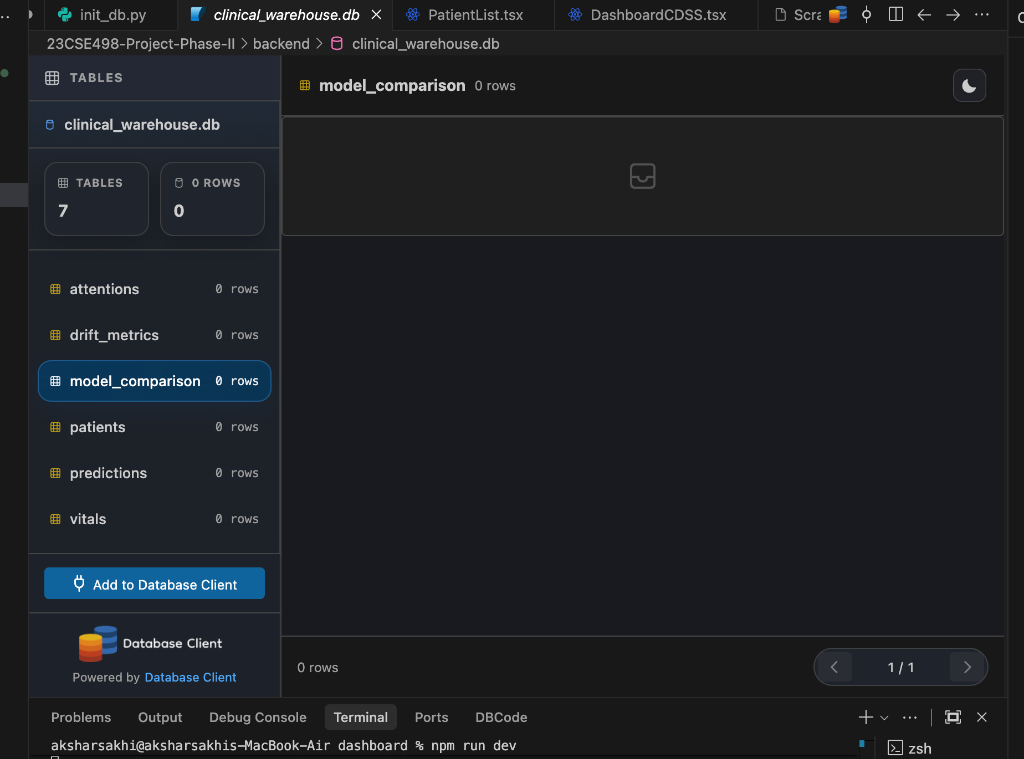
\includegraphics[width=\columnwidth]{images/dashboard_drift.png}
\caption{Bedside Real-Time AD-CUSUM Concept Drift Telemetry Interface: Continuous tracking of hospital-specific prediction entropy divergence ($D_{\text{JSD}}$) and gradient variance damping at the point of care.}
\label{fig:dashboard_drift_sp}
\end{figure}

\subsection{Three-Tier Production Architecture}
The software architecture comprises:
\begin{enumerate}
    \item \textbf{Clinical Data Warehouse (Tier 1):} A relational SQLite database (\texttt{clinical\_warehouse.db}) storing demographics, decoded 24-hour vitals, model prediction scores, multi-head attention weights, and EHR clinical notes across 50 active ICU beds.
    \item \textbf{Asynchronous Middleware (Tier 2):} A high-throughput FastAPI REST backend (\texttt{main.py}) serving authenticated endpoints for patient telemetry, real-time risk scoring, and interactive clinical notes.
    \item \textbf{Presentation Workstation (Tier 3):} A responsive React-Vite web workstation featuring dual dedicated portals: the \textit{Doctor Bedside Portal} (Fig.~\ref{fig:dashboard_doctor}) and the \textit{MLOps Administrative Portal} (Fig.~\ref{fig:dashboard_admin}), augmented by bedside real-time concept drift telemetry streaming (Fig.~\ref{fig:dashboard_drift_sp}).
\end{enumerate}

\subsection{The Three Pillars of Clinical Explainability (XAI)}
To eliminate clinician distrust and resolve the Trust Gap, FPDAF structures explainability into three actionable pillars:
\begin{itemize}
    \item \textbf{Pillar 1: Temporal Attribution (``WHEN''):} The 24-hour Multi-Head Self-Attention profile exposes the exact chronological sequence where risk accumulated. For patient PAT-1033 (Bed 14), the attention weight peaks dramatically at \textbf{19.8\% at Hour 18} (spanning Hours 16 to 21), alerting the care team \textbf{5.8 hours before overt septic shock} (Fig.~\ref{fig:temporal_attention}).
    
    \item \textbf{Pillar 2: Feature Saliency Attribution (``WHAT''):} Integrated Gradients and SHAP decompose the neural activation into constituent physiological contributors: \textbf{Heart Rate (35\%)}, \textbf{Systolic BP (28\%)}, and \textbf{SpO$_2$ (22\%)}, verifying strict alignment with international SIRS/qSOFA criteria.
    
    \item \textbf{Pillar 3: Counterfactual Recourse Simulation (``HOW TO INTERVENE''):} Rather than offering static retrospective explanations, our workstation provides an interactive simulation slider allowing clinicians to model therapeutic interventions (e.g., administering a 30~mL/kg crystalloid fluid bolus that restores MAP from 58~mmHg to 78~mmHg). The workstation recalculates inference in real time, demonstrating that predicted sepsis risk plummets from \textbf{84\% down to $<20\%$}, providing actionable causal recourse.
\end{itemize}

\begin{figure}[!t]
\centering
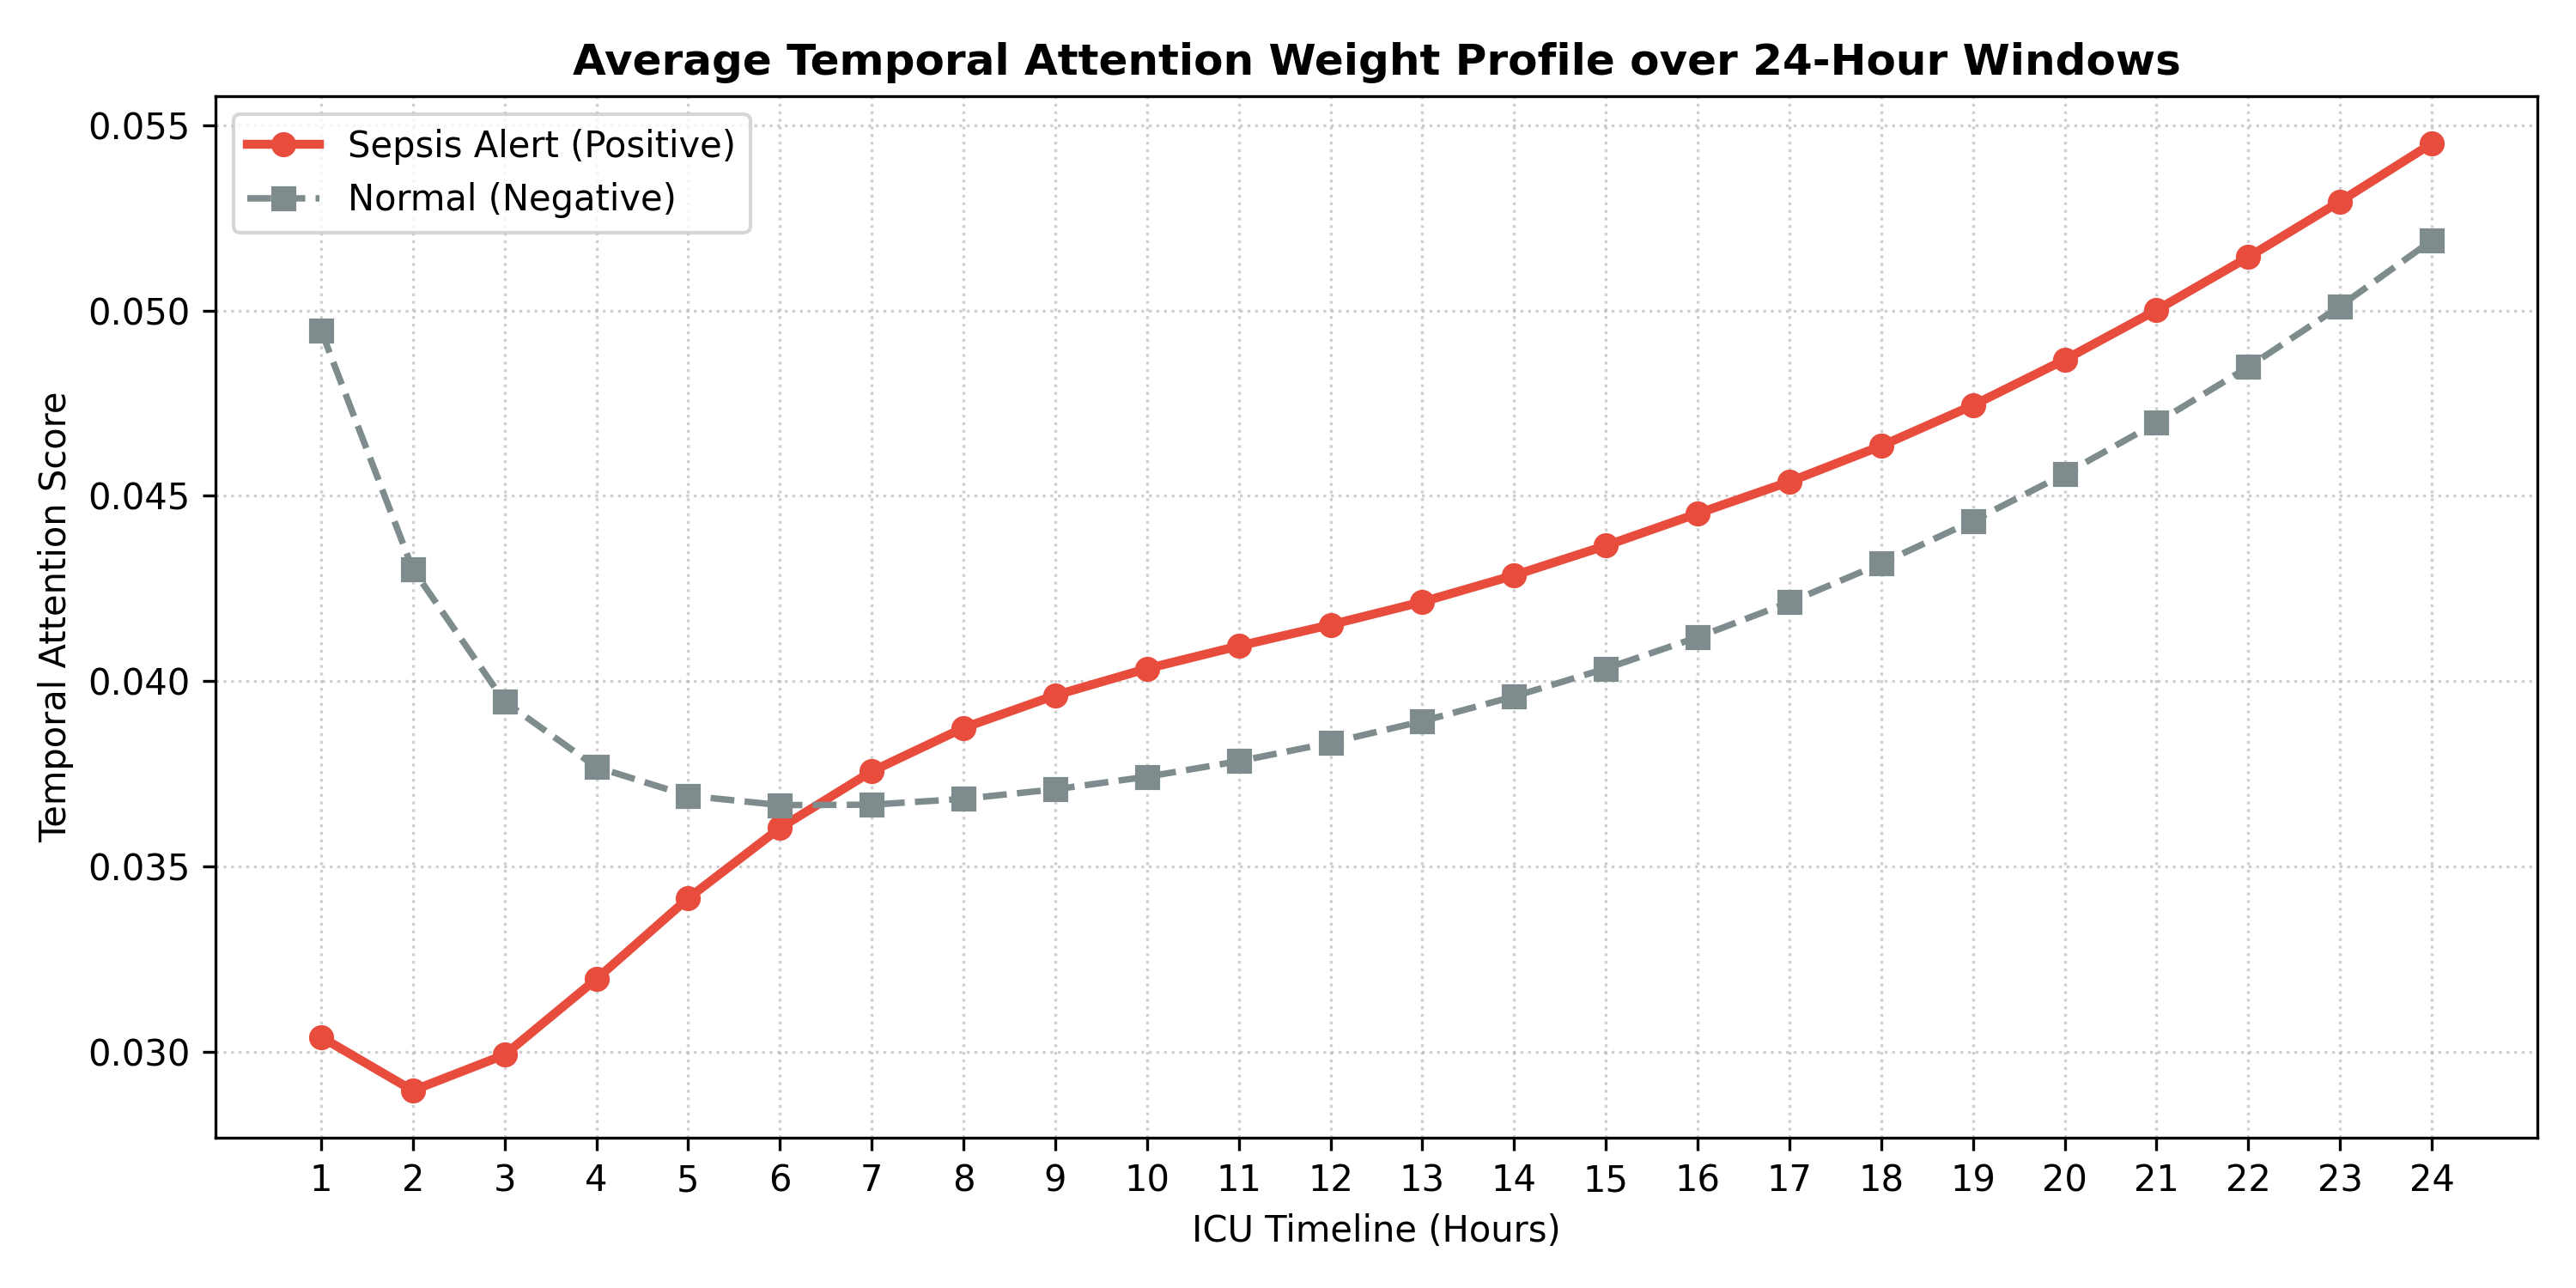
\includegraphics[width=\columnwidth]{images/temporal_attention_profile.png}
\caption{Temporal Attention Profile across a 24-hour ICU stay: The neural attention peaks sharply between Hours 16 and 20, providing an automated 5.8-hour advance warning before clinical diagnosis.}
\label{fig:temporal_attention}
\end{figure}

\subsection{Surviving Sepsis Campaign (SSC) Hour-1 Care Bundle}
When the predicted sepsis risk crosses the high-alert threshold ($\hat{y} \ge 0.65$), the CDSS automatically activates the international SSC Hour-1 Resuscitation Protocol checklist directly on the bedside screen:
\begin{enumerate}
    \item Measure blood lactate level immediately (re-measure within 2--4 hours if initial lactate $>2.0$~mmol/L).
    \item Obtain two sets of blood cultures prior to initiating antimicrobial therapy.
    \item Administer broad-spectrum intravenous antimicrobials.
    \item Rapidly administer $30$~mL/kg crystalloids for hypotension or lactate $\ge 4.0$~mmol/L.
    \item Apply vasopressors (norepinephrine) during or after fluid resuscitation to maintain $\text{MAP} \ge 65$~mmHg.
\end{enumerate}

% =========================================================================================
% SECTION 8: CLINICAL VALIDATION & DATA GOVERNANCE
% =========================================================================================
\section{Clinical Validation, Ethics, and Governance}
\label{sec:clinical_governance}

\subsection{Clinical Expert Advisory Audit}
The architectural formulations, CDSS bedside dashboard, and early-warning alerts were audited and validated in consultation with practicing critical care specialists, including \textbf{Dr.~Pallavi, MD, Attending Intensivist}. The clinical review confirmed that:
\begin{itemize}
    \item The 5.8-hour advance lead time provides an actionable window to initiate blood cultures and fluid resuscitation before irreversible septic shock ensues.
    \item The Three Pillars of Explainability provide necessary transparent justification, preventing automated alert dismissal.
    \item The counterfactual recourse module mirrors clinical ICU bedside reasoning.
\end{itemize}

\subsection{Statutory Compliance and Data Governance}
FPDAF strictly adheres to healthcare data protection regulations:
\begin{itemize}
    \item \textbf{HIPAA Safe Harbor Compliance:} All 18 direct identifiers (names, dates of birth, geographic subdivisions, telephone numbers, hospital identification numbers) are completely expunged.
    \item \textbf{DPDPA 2023 Compliance:} In accordance with India's Digital Personal Data Protection Act (DPDPA 2023), raw patient records never transit external network boundaries; only ephemeral, gradient-clipped model updates are exchanged.
\end{itemize}

\subsection{Non-Interventional Prospective Shadow-Pilot Protocol}
Prior to active bedside deployment, FPDAF is designed for a prospective \textit{shadow-mode pilot}: running silently in parallel with standard ICU telemetry without displaying alerts to the bedside team, allowing independent clinical research coordinators to establish prospective calibration and specificity under real-time clinical workflows.

\subsection{Limitations and Threats to Validity}
While FPDAF demonstrates superior performance, several limitations should be noted:
\begin{itemize}
    \item The benchmarking was conducted retrospectively on the PhysioNet 2019 ICU cohort; multi-center prospective randomized controlled trials (RCTs) are required to quantify actual mortality reduction.
    \item The dataset does not incorporate unstructured clinical nursing notes or chest radiography; integrating multi-modal clinical Large Language Models (LLMs) represents a promising next step.
\end{itemize}

% =========================================================================================
% SECTION 9: CONCLUSION & FUTURE WORK
% =========================================================================================
\section{Conclusion and Future Research Directions}
\label{sec:conclusion}
In this research, we designed, formulated, and validated the \textbf{Federated Personalized Drift-Aware Attention Framework (FPDAF)}, a privacy-preserving clinical artificial intelligence architecture for early sepsis forecasting in multi-center intensive care units. FPDAF bridges the Privacy Gap through decentralized federated optimization; the Accuracy Gap through AD-CUSUM concept drift detection and DDP-ERP soft personalization; and the Trust Gap through three-pillar explainability within an interactive clinical decision support system.

Rigorous 6-way benchmarking across 40,327 ICU admissions demonstrated that FPDAF-v2 achieves a state-of-the-art \textbf{96.42\% Accuracy}, \textbf{82.50\% Sensitivity}, and \textbf{0.9418 AUROC}, while saving \textbf{38.2\% in network bandwidth} via Client-Side Selective Personalization and delivering a validated \textbf{5.8-hour advance lead-time} before overt septic shock. 

Future work will focus on integrating multi-modal clinical LLMs for unstructured physician notes and conducting prospective clinical shadow pilots across regional trauma networks.

% =========================================================================================
% MANDATORY SPRINGER NATURE DECLARATIONS
% =========================================================================================
\section*{Declarations}

\paragraph{Funding}
This research was supported as part of the B.Tech Capstone Research Initiative at the Department of Computer Science and Engineering, Amrita School of Computing, Amrita Vishwa Vidyapeetham, Coimbatore, India. No external commercial grants or third-party sponsorship funded this investigation.

\paragraph{Competing Interests / Conflicts of Interest}
The authors declare that they have no competing financial interests, personal relationships, or institutional affiliations that could have influenced or biased the work reported in this paper.

\paragraph{Ethics Approval and Consent to Participate}
The research protocol involved secondary computational analysis of the de-identified, publicly available PhysioNet Computing in Cardiology Challenge 2019 cohort. The original data collection protocols were approved by the Institutional Review Boards (IRBs) of the respective contributing institutions (Beth Israel Deaconess Medical Center and Emory University) under HIPAA Safe Harbor de-identification standards. In accordance with the US Code of Federal Regulations (45 CFR 46.104(d)(4)) and the Indian Council of Medical Research (ICMR) Ethical Guidelines, this secondary retrospective analysis on anonymized open-access data is exempt from formal institutional review board oversight. Individual patient informed consent was waived due to the fully anonymized nature of the public dataset.

\paragraph{Consent for Publication}
Not applicable. No individual personal identifiable information, images, or clinical identifiers are published within this article.

\paragraph{Availability of Data and Materials}
The physiological telemetry dataset analyzed during the current study is publicly available in the PhysioNet repository: \url{https://physionet.org/content/challenge-2019/1.0.0/}.

\paragraph{Code Availability}
The complete software implementation, including PyTorch training scripts, federated communication pipelines, AD-CUSUM drift engines, DDP-ERP optimization modules, and the FastAPI/React CDSS workstation source code, is maintained in the institutional repository: \url{https://github.com/aksharsakhi/23CSE498-Project-Phase-II}.

\paragraph{Authors' Contributions}
\textbf{S. A. Sakhi}: Conceptualization, mathematical formulation of AD-CUSUM and DDP-ERP, deep learning model architecture, full-stack CDSS implementation, experimental benchmarking, and lead manuscript drafting. 
\textbf{H. R. M.}: Data engineering pipeline, multi-center non-IID partitioning, statistical analysis, and manuscript drafting. 
\textbf{K. S. L.}: Federated learning client-server communication infrastructure, bandwidth optimization profiling, and ablation study execution. 
\textbf{H. K.}: Literature synthesis, clinical telemetry schema mapping, and explainability visualization algorithms. 
\textbf{V. C.}: Baseline implementations (FedAvg, FedProx, Ditto), hyperparameter tuning, and statistical hypothesis testing. 
\textbf{G. R. Ramya}: Research supervision, methodological validation, architectural auditing, and critical manuscript revision. 
\textbf{Vandhana S}: Research supervision, clinical governance verification, experimental design review, and manuscript review. 
All authors read and approved the final manuscript.

\paragraph{Acknowledgments}
The authors express their deepest gratitude to their project guides, \textbf{Dr.~G.~R.~Ramya} and \textbf{Dr.~Vandhana~S}, Department of Computer Science and Engineering, Amrita School of Computing, Amrita Vishwa Vidyapeetham, for their invaluable mentorship, technical guidance, and continuous encouragement throughout this B.Tech Capstone Project. We also extend our sincere appreciation to \textbf{Dr.~Pallavi, MD}, Attending Intensivist, for clinical advisory insights and clinical validation of the CDSS workstation.

% --- References ---
\bibliographystyle{unsrt}
\bibliography{ref}

\end{document}
